
%%%% PREAMBULES %%%%

% 		TO DO des presets :
% fix cref pour les pluriels
% fix les couleurs python de lstlistings
% better mdframed pour les enoncés


%%%%    IMPORTS 2 BASE    %%%%



\documentclass[french, oneside]{article}
\usepackage[utf8]{inputenc}
\usepackage[T1]{fontenc}

% pour le mise en page
\usepackage[a4paper, total={6.5in, 10in}]{geometry}
\usepackage{fontsize} \changefontsize[12]{10}		
\usepackage{xcolor}

% mathsymbole
\usepackage{amsmath, amssymb,stmaryrd}
\usepackage{wasysym}[mathcal] % a quoi sert le [mathcal] ?
\usepackage[nointlimits]{esint} % pour \fint, rien d'autre
\usepackage{nicefrac, units} % fraction pour text mode / unité
%\usepackage{cancel} % pour les simplifications de calcul (trop nice)


% TBD
\usepackage{mathcomp}
\usepackage{mathrsfs} % pour \mathscr a priori

% pour les belles fonts
\usepackage{amsfonts}
\DeclareMathAlphabet{\mathpzc}{OT1}{pzc}{m}{it}
%\usepackage{euscript}[mathcal]
%\usepackage{rsfso}
\usepackage{bbm}	 % mathbb étendu

% pour les hyprlien / cross-ref
\usepackage[pdftitle=Phase~géométrique~de~signal~multivarié,
					   pdfauthor=Grégoire~Doat,
					   %linktoc=all,	%page du TOC clickable
 					   breaklinks=true,	% liens peuvent s'étendre sur plusieurs lignes
 					   colorlinks=true, %colore le 'anchor' text
 					   linkcolor=blue,
 					   citecolor=violet,	
 					   urlcolor=blue]{hyperref}
\usepackage{cleveref}


%pour les figures
\usepackage{graphicx, caption} \usepackage{wrapfig, floatrow}
\usepackage[calc]{adjustbox} %magouille pour wrapfig into ntheorem
%\usepackage{subcaption} % surement useless, parsk floatrow-like 

% pour les beaux tableaux
\usepackage{multirow}
%\renewcommand{\arraystretch}{1.8}

% pour des matrices infernales
\usepackage{easybmat}

% pour plus de liberté sur enumerate
\usepackage{enumitem}
	%[label=\Roman*] dans l'enum env

% pour les citations (aucune idées de comment ca marche)
\usepackage{csquotes}



%%%%    RACCOURCIS    %%%%


% bb / cal / frak
\newcommand{\N}{\mathbb{N}}
\newcommand{\Z}{\mathbb{Z}}  % Note pour homo pour les updates
\newcommand{\Q}{\mathbb{Q}}
\newcommand{\R}{\mathbb{R}}
\newcommand{\C}{\mathbb{C}}
\newcommand{\K}{\mathbb{K}}
\renewcommand{\k}{\Bbbk}
\newcommand{\U}[1]{\text{\normalfont U}(#1)}
\renewcommand{\u}[1]{\mathfrak{u}(#1)}
\newcommand{\A}{\mathbb{A}}
\newcommand{\T}{\mathscr{T}}
\newcommand{\I}{\mathbb{I}}
\renewcommand{\i}{\bf{i}}
\newcommand{\one}{\mathbbm{1}}
%\renewcommand{\S}{\mathfrak{S}}
\renewcommand{\S}[1]{\mathbb{ S}^{#1}}

% arrows
\newcommand{\lr}{\longrightarrow}
\newcommand{\Lr}{\Longrightarrow}
%\renewcommand{\ll}{\longleftarrow}
\newcommand{\Ll}{\Longleftarrow}
\newcommand{\llr}{\longleftrightarrowr}
\newcommand{\Llr}{\Longleftrightarrow}
\newcommand{\lmt}{\longmapsto}

% espaces
\newcommand{\matk}{\mathpzc{M}_n(\mathbb{K})}
\newcommand{\matr}{\mathpzc{M}_n(\mathbb{R})}
\newcommand{\mat}[2][]{\mathpzc{M}_{#1}(#2)}

\newcommand{\Id}[1][]{I_{#1}}
\newcommand{\id}[1][]{id_{#1}}

\newcommand{\sym}[2]{\mathcal{S}_{#1}(#2)}
\newcommand{\asym}[2]{\mathcal{A}_{#1}(#2)}

% fonctions
\newcommand{\Arccos}{\text{\normalfont Arccos}} 
\newcommand{\Arcsin}{\text{\normalfont Arcsin}} 
\newcommand{\Arctan}{\text{\normalfont Arctan}} 
\newcommand{\Argch}{\text{\normalfont Argch}}       
\newcommand{\Argsh}{\text{\normalfont Argsh}}

\newcommand{\transp}[1]{{#1}^\top}
\newcommand{\congu}[1]{\overline{#1}}

\newcommand{\argmin}[1]{\underset{#1}{\text{\normalfont argmin}}}
\newcommand{\argmax}[1]{\underset{#1}{\text{\normalfont argmax}}}
\newcommand{\supp}{\text{\normalfont supp}\,}

\newcommand{\pgcd}{\text{\normalfont pgcd}}
\newcommand{\PGCD}{\text{\normalfont PGCD}}
\newcommand{\ppmc}{\text{\normalfont ppcm}}
\newcommand{\sign}{\text{\normalfont sign}}

\newcommand{\sgn}{\text{\normalfont sgn}}
%\newcommand{\deg}{\text{deg}}
\newcommand{\ord}{\text{\normalfont ord}}

%\renewcommand{\det}{\text{det}}
\newcommand{\tr}{\text{\normalfont tr}}
\newcommand{\rg}{\text{\normalfont rg}}
\newcommand{\Co}{\text{\normalfont com}}
\newcommand{\codim}{\text{\normalfont codim}}

%\renewcommand{\div}{\text{div}}
%\newcommand{\rot}{\text{\normalfont rot}}

%espaces
\renewcommand{\vec}{\text{Vec}}
\newcommand{\im}{\text{\normalfont Im}}
\newcommand{\Ker}{\text{\normalfont Ker}}
\newcommand{\Ann}{\text{\normalfont Ann}}
\newcommand{\Sp}{\text{\normalfont Sp}} 
\newcommand{\GL}{\text{\normalfont GL}}
\newcommand{\SL}{\text{\normalfont SL}}
\newcommand{\SO}{\text{\normalfont SO}}
\newcommand{\SU}{\text{\normalfont SU}}

\newcommand{\Aff}{\text{\normalfont Aff}}
\newcommand{\HT}{\text{\normalfont HT}}
\newcommand{\GA}{\text{\normalfont GA}}

\newcommand{\conti}[3][]{\mathscr{C}^{#1}\left(#2,#3\right)}

% spé proba
\newcommand{\esp}[2][]{\mathbb{E}_{#1}\left[\, #2\, \right]}
\newcommand{\var}[2][]{\mathbb{V}_{#1}\left[\, #2\, \right]}

% plus jolie
\renewcommand{\O}{\varnothing}
\renewcommand{\epsilon}{\varepsilon}
\renewcommand{\subsetneq}{\varsubsetneq}
\renewcommand{\leq}{\leqslant}
\renewcommand{\geq}{\geqslant}
\renewcommand{\limsup}{\varlimsup}
\renewcommand{\liminf}{\varliminf}

% autre
\newcommand{\defeq}{:=}
\renewcommand{\bf}[1]{\boldsymbol{#1}}
%\renewcommand{\AC}{\sim}
\newcommand{\para}{\sslash}

% latin
\newcommand{\etal}{\textit{et al.}}
\newcommand{\etc}{\textit{etc.}}
\newcommand{\apriori}{\textit{a priori}}
\newcommand{\Apriori}{\textit{A priori}}
\newcommand{\afortiori}{\textit{a fortiori}}
\newcommand{\Afortiori}{\textit{A fortiori}}
\newcommand{\acontrario}{\textit{a contrario}}
\newcommand{\infine}{\textit{in fine}}
\newcommand{\ie}{\textit{i.e.}}
\newcommand{\eg}{\textit{e.g.}}
\newcommand{\cf}{\textit{cf.}}

% tmp (notation)

\newcommand{\x}{\bf{x}}
	%phase
\newcommand{\phaset}{\Phi_{\text{\normalfont tot}}}
\newcommand{\phased}[1][]{\Phi_{\text{\normalfont dyn}\, #1}}
\newcommand{\phaseg}{\Phi_{\text{\normalfont geo}}}
\newcommand{\phasei}{\Phi_{\text{\normalfont inst}}}

	% analyse temps-fréquence
\newcommand{\densit}{\rho}
\newcommand{\densis}{\varrho}
\newcommand{\Fou}[1]{\mathcal{F}\left[#1\right]}
\newcommand{\fou}[1]{\hat{#1}}
\newcommand{\iFou}[1]{\mathcal{F}^{-1}\left[#1\right]}
\newcommand{\SA}[1]{\mathcal{A}\left[#1\right]}
\newcommand{\sa}[1]{#1_+}
\newcommand{\hilb}[1]{\mathcal{H}\left[#1\right]}

\newcommand{\vpC}{\text{\normalfont vp} \frac{1}{x}}
\newcommand{\barint}[2][]{\text{\sout{\ensuremath{\displaystyle \int_{#2}}}}^{#1}}

	% writing progress
\newcommand{\thoughts}[1]{{\itshape\color{red}#1}}
\newcommand{\wip}{{\color{violet}$\bf{*}$\ \ }}
\newcommand{\todo}{{\color{red}$\bf{*}$\ \ }}
\newcommand{\DONE}{{\color{red}DONE\ }}
\newcommand{\new}{{\color{yellow}$\bf{*}$\ \ }}

	%variétoche
\newcommand{\manu}{\mathpzc{M}}
\newcommand{\atls}{\mathscr{A}}
\newcommand{\bt}{\bf{\partial}}

\newcommand{\tg}[2][]{T_{#1}#2}%{\text{\normalfont T}_{#1}#2}
\newcommand{\vg}[2][]{V_{#1}#2}%{\text{\normalfont V}_{#1}#2}
\newcommand{\hg}[2][]{H_{#1}#2}%{\text{\normalfont H}_{#1}#2}
\newcommand{\ver}{\text{\normalfont ver}}
\newcommand{\hor}{\text{\normalfont hor}}

\newcommand{\VFP}{\S{n}\big(\U{1},\PC{n}\big)}

\newcommand{\conn}{\omega}
\newcommand{\locconn}{\mathcal{A}}

\renewcommand{\d}{\text{\normalfont d}}

\renewcommand{\dim}[1][]{\text{\normalfont dim}_{#1}}
%\newcommand{\dimC}[]{\text{\normalfont dim}_{\C}}

\newcommand{\PC}[1]{\text{\normalfont P}\mathbb{C}^{#1}}
\newcommand{\Hol}{\text{\normalfont Hol}}

\newcommand{\pr}[1]{\text{\normalfont pr}_{#1}}
\newcommand{\concat}[2]{#1 \smallfrown #2} %{\overset{\frown}{#1 #2}}

%ultre-cursed (fix asap)
\newcommand{\skipl}{{\color{white}l}}


%%%%    ENONCES (PROP, DEF, RQ)    %%%%


%\usepackage{amsthm}
\usepackage[hyperref, noconfig]{ntheorem}
\usepackage[ntheorem, framemethod=tikz]{mdframed}


% les styles
\definecolor{colorbar}{rgb}{1.0, 0.55, 0.0}%{255,223,0}
%\definecolor{colorbar}{HTML}{ffd700}
\mdfdefinestyle{barred}{leftmargin=0.15cm, rightmargin=-0.2cm,
	skipabove=15pt, skipbelow=150pt, 		% tailles des marges
	linewidth=0.03cm, linecolor=black, 	% box' style
	topline=false, bottomline=false,
	rightline=false, leftline=true}		% coté de la box

\mdfdefinestyle{ramark}{leftmargin=0.4cm, rightmargin=0.4cm, 
	skipabove=5pt, skipbelow=5pt,
	topline=false, bottomline=false, rightline=false, leftline=false}
	
\mdfdefinestyle{demo frame}{leftmargin=0.15cm, rightmargin=0.7cm, 
	skipabove=5pt, skipbelow=0pt,	
	linewidth=0.4pt, linecolor=black,
	topline=false, bottomline=false, rightline=false, leftline=false}

% théorèmes (pour pouvoir les nommer)
\makeatletter
	\newtheoremstyle{theo}{\scshape ##1 ##2\quad ---\quad}{{\scshape##1 ##3 (##2)\quad ---\quad}}
\makeatother
\theoremstyle{theo}
\theorembodyfont{\normalfont}
\newmdtheoremenv[style=barred]{theoreme}{Théorème}

% énoncés classiques
\theoremstyle{plain}
\theoremheaderfont{\scshape}
\theoremseparator{\ \ ---\ \ }
\theoremnumbering{arabic}
\theorembodyfont{\normalfont}


\newmdtheoremenv[style=barred]{definition}{\indent Définition}%[section]
\newmdtheoremenv[style=barred]{proposition}{\indent Proposition}
\newmdtheoremenv[style=barred]{propriete}{\indent Propriété}
\newmdtheoremenv[style=barred]{propricarac}[propriete]{\indent Propriété Caractéristique}
\newmdtheoremenv[style=barred]{lemme}{\indent Lemme}
\newmdtheoremenv[style=barred]{theodef}[theoreme]{\indent Théorème et Définition}
\newmdtheoremenv[style=barred]{corollaire}{\indent Corollaire}[theoreme]

% énoncé type
\makeatletter
	\newtheoremstyle{special}{##1 ##2}{{\scshape ##3}\quad ---\quad}
\makeatother
\theoremstyle{special}
\theoremheaderfont{\scshape}
\theoremseparator{\ \ ---\ \ }
\theoremnumbering{arabic}
\theorembodyfont{\normalfont}

\newmdtheoremenv[style=barred]{enonce}{}

% énoncé numérotation-less
\theoremstyle{nonumberplain}
\theoremheaderfont{\normalfont\scshape}
\theoremseparator{}
\theoremnumbering{arabic}
\theorembodyfont{\normalfont\itshape}

\newmdtheoremenv[style=ramark]{remarque}{\indent}
\newtheorem{rappel}{\indent Rappel}
\newtheorem{exemple}{\indent Exemple}

% exos
\theoremstyle{break}
\theoremheaderfont{\bfseries\scshape\color{blue}}
\theoremseparator{ : }
\theoremnumbering{arabic}
\theorembodyfont{\normalfont}
\newtheorem{exercice}{Exercice}

% demo
\theoremstyle{empty}
\theoremheaderfont{\itshape}
\theoremseparator{\quad ---\quad}
\theoremnumbering{arabic}
\theorembodyfont{\normalfont}

\newmdtheoremenv[style=demo frame]{demonstration}{Démonstration}

\newenvironment{demo}[1][\unskip]{%
	\vspace{0.5cm} \hspace{-0.55cm}\textbf{\textit{Démonstration #1}} \qquad %\rule{5cm}{0.4pt}
	\begin{demonstration}%
	}{\begin{flushright} $\blacksquare$ \end{flushright}
	\end{demonstration}}


	% pour cref aux enoncés
	
%no cap
\crefname{definition}{définition}{définitions}
\crefname{proposition}{proposition}{propositions}
\crefname{propriete}{propriété}{propriétés}
\crefname{lemme}{lemme}{lemmes}
\crefname{theoreme}{théorème}{théorèmes}
\crefname{corollaire}{corollaire}{corollaires} 

\crefname{remarque}{remarque}{remarques}
\crefname{rappel}{rappel}{rappels}
\crefname{exemple}{exemple}{exemples}

\crefname{exercice}{exercice}{exercices}
%cap
\Crefname{definition}{\textit{def.}}{\textit{def.}}
\Crefname{proposition}{Proposition}{Propositions}
\Crefname{propriete}{Propriété}{Propriétés}
\Crefname{lemme}{Lemme}{Lemmes}
\Crefname{theoreme}{Théorème}{Théorèmes}
\Crefname{corollaire}{Corollaire}{Corollaires} 

\Crefname{remarque}{Remarque}{Remarques}
\Crefname{rappel}{Rappel}{Rappels}
\Crefname{exemple}{Exemple}{Exemples}

\Crefname{exercice}{Exercice}{Exercices}



%%%%    PROG N PLOT    %%%%


% Prog

%\usepackage{fancyvrb} % pour le lore, mais useless AF
\usepackage{listings} 
%\usepackage{pythontex}	% surement une dingz, à approfondire

% preset
\definecolor{codeblack}{gray}{0.2}
\definecolor{codegreen}{rgb}{0,0.6,0}
\definecolor{codegray}{gray}{0.5}
\definecolor{codepurple}{rgb}{0.58,0,0.82}
\definecolor{backcolour}{rgb}{0.90,0.90,0.87}

\lstdefinestyle{mystyle}{
	backgroundcolor=\color{backcolour},   
	commentstyle=\color{codegray},
	keywordstyle=\color{orange},
	numberstyle=\tiny\color{codegray},
	stringstyle=\color{codegreen},
	basicstyle=\color{codeblack}\ttfamily\footnotesize,
	breakatwhitespace=false,         
	breaklines=true,                 
	captionpos=b,
	abovecaptionskip=12pt,
	belowcaptionskip=18pt,
	keepspaces=true,                 
	numbers=left,                    
	numbersep=5pt,                  
	showspaces=false,                
	showstringspaces=false,
	showtabs=false,                  
	tabsize=2,
	frame=single,
	rulecolor=\color{lightgray}}
\newcommand{\pyt}[1]{\colorbox{backcolour}{ {\color{codeblack}\footnotesize \texttt{#1}}}}
\newcommand{\lin}[1]{({\color{black}\footnotesize\texttt{#1}})}

\lstset{style=mystyle}


% Plot

% pour dessins et les diagrams
\usepackage{tikz, tikz-cd, tkz-euclide}
\usepackage{scalerel, pict2e}
\usetikzlibrary{calc, patterns, decorations, shapes.arrows, arrows.meta, shadows, external} 

\tikzcdset{every label/.append style = {scale=1.0 ,yshift=0.6ex},
	every matrix/.append style={nodes={font=\small}}}

% pour les maxis plots
\usepackage{pgfplots}
\pgfplotsset{compat=newest, scaled y ticks=false}
\usepgfplotslibrary{groupplots, dateplot, statistics, fillbetween}

\tikzstyle{every node}=[font=\scriptsize]
\pgfplotsset{standard/.style={width=8cm,
	height=3cm,
	compat=1.18,
	trig format=rad,
	enlargelimits,
	axis x line=middle,
	axis y line=middle,
	enlarge x limits=0.15,
	enlarge y limits=0.15,
	every axis x label/.style={footnotesize, at={(current axis.right of origin)},anchor=north west},
	every axis y label/.style={footnotesize, at={(current axis.above origin)},anchor=south east},
	scale only axis=true}}



%%%%    CAPTIONS 2 FIGURES    %%%%


% set up des captions figures (extrêmement BG)

% pos et séparateur générale
\captionsetup{justification=centering}
\DeclareCaptionLabelSeparator{custom}{\, ---\, }
%\DeclareCaptionFormat{custom}{#1#2#3}

% spécial figure
\DeclareCaptionLabelFormat{customfig}{fig. #2}
\captionsetup[figure]{font=it, labelformat=customfig, labelsep=custom}

% spécial tableau
\DeclareCaptionLabelFormat{customtab}{tab. #2}

\captionsetup[table]{font=it, labelformat=customtab, labelsep=custom}

% spécial code (listings)
\DeclareCaptionLabelFormat{customcode}{code #2}

\captionsetup[lstlisting]{font=it, labelformat=customcode, labelsep=custom}

% pour cref
\crefname{figure}{\itshape fig.}{\itshape fig.}
\crefname{table}{\itshape tab.}{\itshape tab.}

\Crefname{figure}{figure}{figures}
\Crefname{table}{tableau}{tableaux}
	
	
	
	
%%%%    TABLES/REF  &  HAUT/BAS DE PAGES    %%%%


% nom des tables et références

\renewcommand{\contentsname}{\begin{center}\textsc{Tables des Matrières} \end{center}}
\renewcommand{\listfigurename}{\begin{center}\textsc{Table des Figures}\end{center}}
\renewcommand{\lstlistlistingname}{\begin{center}\textsc{Table des Codes}\end{center}}
\renewcommand{\refname}{\begin{center}\textsc{Références}\end{center}}

% bas/haut de page (à optimiser à l'occas')

\usepackage{fancyhdr}
\pagestyle{fancy}                       
\fancyhf{}
\renewcommand{\headrulewidth}{0pt}
\cfoot{\thepage}

%version2réjane  :
%\usepackage{eso-pic}
%\renewcommand\headrulewidth{1pt}
%\fancyhead[L]{\includegraphics[width=3cm]{logo_lr.png}}
%\fancyhead[R]{\includegraphics[width=1cm]{logo_sdis17.png}}
%\setlength{\headsep}{45pt}



%%%%    SECTIONS ET TOC    %%%%

	
	% génération des sections
	
\usepackage[loadonly, clearempty, newparttoc, toctitles]{titlesec}

% liste des sections
\titleclass{\part}[0]{top} % 0 = niveau de section
\titleclass{\section}{straight}[\part]
\titleclass{\subsection}{straight}[\section]
\titleclass{\subsubsection}{straight}[\subsection]

\makeatletter % pour que les sections suivent les parts
	\@addtoreset{section}{part} % (jsp pk ca marche pas sinon :/)
\makeatother


% formatage
\titleformat{\part}[display]{\bfseries\scshape\Large}{\centering \rule{3.5cm}{0.4pt}\qquad Partie\quad \thepart \qquad \rule{3.5cm}{0.4pt}}{15pt}{\centering}[\vspace{0.2cm}\rule{8cm}{0.4pt}]
\titlespacing{\part}{0pt}{50pt}{70pt}
\newcommand{\partbreak}{\clearpage}

\titleformat{\section}{\bfseries\Large}{\thesection\quad ---}{15pt}{}
\titlespacing{\section}{10pt}{20pt}{15pt}
%\newcommand{\sectionbreak}{\clearpage}

\titleformat{\subsection}{\bfseries\large}{\thesubsection}{15pt}{}
\titlespacing{\subsection}{20pt}{15pt}{15pt}

\titleformat{\subsubsection}{\bfseries}{\thesubsubsection}{15pt}{}
\titlespacing{\subsubsection}{30pt}{15pt}{15pt}

% pour cref aux enoncés
\crefname{part}{partie}{parties}
\crefname{section}{section}{sections}
\crefname{subsection}{section}{sections}
\crefname{subsubsection}{sous-section}{sous-sections}
	% pour cref version short
\Crefname{part}{\textit{pt.}}{\textit{pt.}}
\Crefname{section}{\textit{sec.}}{\textit{sec.}}
\Crefname{subsection}{\textit{sec.}}{\textit{sec.}}
\Crefname{subsubsection}{\textit{ss-sec.}}{\textit{ss-sec.}}


	% le TOC en lé-gende

\usepackage{titletoc}
%\contentsmargin{2em}

\titlecontents{part}[2em]{\bfseries\large\scshape 
	\hspace*{-1.5em}\rule{\textwidth}{0.5pt}\vspace{0.1cm}\\*
	 }{Partie\quad \contentslabel{-0.05em}\quad\ ---\quad}{\contentslabel{-1.5em} ---\quad }{\hfill\contentspage}[\hspace*{-0.5em}
\rule{\textwidth}{0.5pt}]

\titlecontents{section}[1.5em]{\addvspace{1em}\bfseries}{\contentslabel{1.25em} ---\quad}{\hspace*{-1.75em}}{\titlerule*[0.75pc]{.}\contentspage}[\addvspace{0.25em}]

\titlecontents{subsection}[3.8em]{\addvspace{0.15em}\normalfont}{\contentslabel{2em}}{\hspace*{-2em}}{\titlerule*[0.75pc]{.}\contentspage}

\titlecontents{subsubsection}[6.8em]{\normalfont}{\contentslabel{2.75em}}{\hspace*{-2.5em}}{\titlerule*[0.75pc]{.}\contentspage}


% set up d'un environnement pour les annexes

\newenvironment{annexe}{%
	\newpage
	
	% changement title sec
	\titleformat{\section}[display]{\bfseries\scshape\Large}{\centering}{15pt}{\centering}
	\titlespacing{\section}{0pt}{30pt}{40pt}
	
	\titleformat{\subsection}{\bfseries\large}{Annexe \thesubsection\quad ---\quad}{0pt}{}
	
	\titleformat{\subsubsection}{\bfseries}{\thesubsubsection}{15pt}{}
	
	% changement title toc
	\titlecontents{section}[0.25em]{\addvspace{0.5em}\bfseries }{}{\hspace*{-1.5em}}{\titlerule*[0.75pc]{.}\contentspage}
	
	\titlecontents{subsection}[1.75em]{\normalfont Annexe \hspace*{1.5em}}{\contentslabel{1.25em} ---\quad}{\hspace*{-2em}}{\titlerule*[0.75pc]{.}\contentspage}
	
	\titlecontents{subsubsection}[6em]{\normalfont}{\contentslabel{2.75em}}{\hspace*{-2em}}{\titlerule*[0.75pc]{.}\contentspage}
	
	% changment de la numéritations
	\renewcommand{\thesubsection}{\Alph{subsection}}
	\renewcommand{\thesubsubsection}{\Alph{subsection}.\arabic{subsubsection}.}
	% mise à zéro des compters
	%\setcounter{section}{0}
}{
\titlecontents{section}[1.5em]{\addvspace{1em}\bfseries}{\contentslabel{1.25em} ---\quad}{\hspace*{-1.75em}}{\titlerule*[0.75pc]{.}\contentspage}[\addvspace{0.25em}]

\titlecontents{subsection}[3.8em]{\addvspace{0.15em}\normalfont}{\contentslabel{2em} ---\quad}{\hspace*{-2em}}{\titlerule*[0.75pc]{.}\contentspage}

\titlecontents{subsubsection}[6.8em]{\normalfont}{\contentslabel{2.75em}}{\hspace*{-2.5em}}{\titlerule*[0.75pc]{.}\contentspage}}




%%%%    COMPTEUR ET NUMEROTATIONS    %%%%


	% Sections
\renewcommand{\thepart}{\Roman{part}}

\numberwithin{section}{part}
\renewcommand{\thesection}{\Roman{section}}

\renewcommand{\thesubsection}{\arabic{section}.\arabic{subsection}}
\renewcommand{\thesubsubsection}{\arabic{section}.\arabic{subsection}.\arabic{subsubsection}}

	% Equation
\numberwithin{equation}{part}
\renewcommand{\theequation}{\arabic{part}.\arabic{equation}}

\crefname{equation}{\itshape eq.}{\itshape eqs.}
\Crefname{equation}{équation}{équations}

	% Figure
\numberwithin{figure}{part}
\renewcommand{\thefigure}{\itshape\arabic{part}.\arabic{figure}}

%\numberwithin{table}{part}
%\renewcommand{\thetable}{\itshape\arabic{part}.\arabic{table}}

% /!\ à placer après le \begin{document} :
%\numberwithin{lstlisting}{part}
%\renewcommand{\thelstlisting}{\itshape\arabic{part}.\arabic{lstlisting}}



\begin{document}	
%\numberwithin{lstlisting}{part}
%\renewcommand{\thelstlisting}{\itshape\arabic{part}.\arabic{lstlisting}}
	
%%%% PAGE DE GARDE %%%%


\begin{titlepage}
	%\AddToShipoutPictureBG*{\put(80,655){%\includegraphics[width=2.9cm]{Logo MIX.png}}}
	%\AddToShipoutPictureBG*{\put(70,738){%\includegraphics[width=5cm]{logo_lr.png}}}
	%\hspace{0.0cm} 
	%\AddToShipoutPictureBG*{\put(440,690){%\includegraphics[width=3.0cm]{logo_sdis17.png}}}\\[5.0cm]
	%{\color{white}l}\par
	
	\centering
	\vspace{1.5cm}
	{\huge\textbf{Mémoire de Stage de M2}}\par
	
	\vspace{2cm}
	{\huge\textbf{\textsc{Phase Géométrique de Signal Multivarié}}}\par 
	\vspace{0.5cm}
	
	{\huge\textbf{\textsc{... et puis c'est déjà pas mal}}}\par
	\vspace{2.0cm}
	
	{\large Grégoire \textsc{Doat}}\par
	\vspace{0.5cm}
	\vfill
	
	% Bottom of the page
	{\large Encadré par Nicolas \textsc{Le Bihan}, Pierre-Olivier \textsc{Amblard}, Julien \textsc{Flamant} \& Michel \textsc{Berthier}}\par
	\vspace{0.5cm}
	
	\rule{10cm}{0.4pt}\par
	\vspace{0.7cm}
	
	{Master \textsc{Mix} -- Université de La Rochelle}\par
	\vspace{0.25cm}
	
	{\large 2024 -- 2025}
\end{titlepage}



%\newpage

\tableofcontents\thispagestyle{empty}

\skipl \\ \\ \\

\wip : \textsc{partiellement terminée}

\todo : \textsc{au stade de note}
\\ \\
\textsc{Tout les textes en rouges sont des notes. Les figures avec leur caption sont pour la plus part à faire (mise en page comprise).}
\\ \\
\textsc{Les nouveautés : }
\begin{itemize}
	\item J'ai écrit la conclusion de la partie I et l'intro de la partie II (même si j'en suis moyennement convaincu). Dedans j'ai mis au clair les notations $\ S^{2n\pm1}$ vs $\S{n}$
	
	\item J'ai un peu changé le plan de la partie II (à voir si ca vous plaît)
	
	\item La section 1. de la partie II à pas trop changé mais normalement elle devrait être plus claire. Par contre dans la section 2. j'ai pas mal retouché. 
	
	\item J'ai essayé d'avancé la dernière sous partie (2.3, géodésique + préparation du terrain pour Bargmann) mais je bloque encore sur les calculs à cause du $\pi$ (même si j'essaye de l'ignorer) pour les géodésique et du facteur 1/2 qui me manque avec Stokes.
	
	\item J'ai dû, un peu malgré moi, me pencher sur les histoires de double cover pour être sur que ca soit pas dû à ca et ca à pas l'aire (par contre j'ai trouvé deux ref qui ont l'air vraiment bien la dessus : \href{https://www.youtube.com/watch?v=Ay482u6b3Xo&t=959s}{cette vidéo} et \cite{woit_quantum_2017})
	\\
	Faudra qu'on parle de ca ensemble demain pro mais en attendant je pense que je vais juste me lancer sur la partie 3, parce que je suis grave à la bourre là et j'ai trop galéré à avancer cette semaine...
\end{itemize}


\newpage

\setcounter{page}{1}






%%%% INTRO DU MEMOIRE %%%%

\phantomsection
\addcontentsline{toc}{section}{Introduction \& préambule}
\section*{\begin{center}\scshape Introduction \end{center}}


La phase géométrique fait partie de ces concepts qui apparaissent régulièrement en physique, mais qui nécessite beaucoup de contexte pour être mis en évidence.
Pour l'introduire rapidement, la phase géométrique à l'instant $t$ d'un signal multivarié complexe (\ie~à valeurs dans $\C^n$) $\x$ est donnée par :
\[\phaseg(\x, t_0, t) = \arg\big\langle \x(t), \x(t_0)\big\rangle - \Im m\int_{t_0}^t \frac{\big\langle \dot{\x}(s) , \x(s) \big\rangle}{\|\x(s)\|^2} ds\]
Ce qui rend cette phase si intéressante c'est qu'elle est invariante par transformation de jauge, c'est-à-dire invariante par toute transformation du type :
\[\x(t)\ \leadsto\ \x'(t) = e^{i\alpha(t)}\x(t) \]
\\
Elle est également invariante par reparamétrisation et pour ces raisons, c'est une mesure qui est intrinsèquement liée à la trajectoire du signal dans l'espace, à sa géométrie.
\\

La phase géométrique est un phénomène qui apparaît dans de nombreuses circonstances, en fonction desquelles elle peut changer de nom et de forme : phase de Pancharatnam, de Berry, d'Aharonov-Anandan, d'Aharonov-Bohm, angle de Hannay, \etc
\\
L'article \cite{cohen_geometric_2019} de Cohen \etal~en présente quelques unes et le livre ``\textit{Geometric Phases in Classical and Quantum Mechanics}'' \cite{chruscinski_geometric_2004} de Chru\'sci\'nski \& Jamio\l kowski en fait une description plus qu'extensive.
\\

Du point de vue du traitement du signal en revanche, rien n'a été fait et ce n'est que récemment que Le Bihan, Flamant \& Amblard s'y sont intéressés \cite{le_bihan_modephysiques_2023, le_bihan_geometric_2024}.
L'objectif de ce mémoire est donc de décrire la phase géométrique dans le cadre du traitement du signal et de discuter de ses applications :
\\
\begin{itemize}
	\item Dans un premier temps (\cref{part:param_instant}), cette phase sera mise en évidence à travers des concepts d'analyse temps-fréquence, notamment la notion de fréquence instantanée qui sera présente tout au long de l'écrit. 
	Suite à quoi elle sera explicitement calculée dans un cas particulier de signaux, déjà étudié par Le Bihan \etal~\cite{le_bihan_geometric_2024} : les signaux AM-FM-PM.
	Cela permettra de mieux comprendre son comportement et permettra de motiver une description des signaux multivariés complexes dans l'esprit de l'analyse temps-fréquence.
	
	\item Cela mènera à travailler dans une variété dite fibrée principale, $S^{2n-1} \big(\U{1}, \PC{n-1}\big)$, et la seconde partie de ce mémoire sera dédiée à son formalisme. Contrairement à l'état de l'art, les résultats seront présenté d'un point de vue de mathématicien plus que de physicien et, entre autre, l'accent sera mis sur l'intuition géométrique derrière les concepts abordés.
	Des résultats, connus par ailleurs, sur la phase géométrique seront redémontrés avec ce formalisme et avec, les notions de fréquences instantanées et de phase géométrique seront reformulée et réinterprétée. 
	
	\item Enfin, dans une troisième partie, sera présenté un moyen de calculer la phase géométrique en pratique via l'invariant de Bargmann, tiré de \cite{rabei_bargmann_1999} et déjà repris par Le Bihan \etal~\cite{le_bihan_geometric_2024}. Seront ensuite discutées diverses applications \thoughts{et là ça dépend d'à quel point j'ai le temps}.
\end{itemize}





\newpage

%\phantomsection
%\addcontentsline{toc}{section}{Préambule}
\section*{\begin{center}\scshape \todo Préambule \end{center}}\label{sec:index_nota}

\thoughts{Juste des notes, même pas sur qu'il y ait vraiment besoin de garder ce préambule}
\\ \\
Généralités :
\begin{itemize}
	
	\item Les références sont en fin de mémoire est en .bib sur le \href{https://github.com/GregoireDoat/StageM2}{GitHub}
	
	\item Idem pour les codes et un mot sur \texttt{pygeomphase}

	\item On va parler de géo diff et pour éviter de réécrire un livre, on va admettre beaucoup de résultats, on renvoi vers \cite{lafontaine_introduction_2015,do_carmo_riemannian_1992} pour les bases et  \cite{nakahara_geometry_2003,pham_mau_quan_introduction_1969,ballmann_lectures_2006} pour toute ce qui est variété fibrée principales et variétés complexes.
	
	%\item ne seront numérotées que les équations importants
\end{itemize}
\skipl

Notations math :
\begin{itemize}
	
	\item Convention sur le produit hermitien (congué à droite)
	
	\item les vecteurs seront en gras, leur dérivée en temps notée par un point (ex. : $\dot{\x}(t)$) et celle des scalaires seront noté par un prime (ex. : $a'(t)$)
	
	%\item convention de sommation d'Einstein ? (oui mais est-ce qu'on en parle maintenant)
\end{itemize}
\skipl



\newpage

%\tableofcontents\thispagestyle{empty}





%%%% COEUR DU MEMOIRE %%%%


\part{Introduction de la Phase Géométrique} \label{part:param_instant} 
En traitement du signal, la phase d'un signal est intrinsèquement liée à la notion de fréquence instantanée, qui joue un rôle important en analyse temps-fréquence. 
C'est donc de ce point que commencera notre discussion pour introduire la phase géométrique.
Pour cela, seront rapidement introduites quelques notions et résultats d'analyse temps-fréquence dans le cas univarié (sec. \ref{subsec:ana_temp-freq}). Suite à quoi, une notion de phase instantanée sera proposée dans le cas multivarié (sec. \ref{subsec:intro_phased}), ce qui permettra, enfin, de mettre en évidence la phase géométrique (sec. \ref{subsec:intro_phaseg}).
\\

Dans une seconde partie, seront introduits les signaux bivariés dits AM-FM-PM, dont la phase géométrique sera calculée explicitement (sec. \ref{subsec:AM-FM-PM}), ce qui permettra de mettre en évidence certaines de ses propriétés (sec. \ref{subsec:phase_g2Poincare}). Dans une dernière section, seront proposées des généralisations des signaux AM-FM-PM au delà du cas bivarié (sec. \ref{subsec:aller_plus_loin}), ce qui mènera au formalisme de la \cref{part:phase_geo} suivante.
\\




\section{Introduction de la phase géométrique} \label{sec:intro_phaseg}

\subsection{Un peu d'analyse temps-fréquence} \label{subsec:ana_temp-freq}

En traitement du signal, l'analyse fréquentielle par la transformée de Fourier est un incontournable. 
Seulement, cette transformation fait perdre toute notion temporelle : si l'étude du spectre du signal permet de dire quelles fréquences apparaissent dans le signal, elle ne permet pas de dire à quel(s) moment(s). 
C'est en réponse à cela, entre autre, que fut développée l'analyse temps-fréquence et, à cette fin, sont définis les paramètres instantanées d'un signal :\par

\begin{definition}[Paramètres instantanés] \label{def:param_instant}
	Soit $x$, est un signal complexe écrit sous forme exponentielle :
	\begin{align}
		x\ &:\ \begin{aligned}\R\ &\lr\qquad \C \\
			t\ &\longmapsto\ a(t)e^{\i \phi(t)}
		\end{aligned}  &  \text{où }\quad a(t)\in\R^+\quad &\text{et}\quad \phi(t)\in\R
	\end{align}
	$a$ est appelé \emph{amplitude instantanée} du signal, la dérivée $\nicefrac{1}{2\pi}\phi'$ sa \emph{fréquence instantanée} et sa \emph{phase instantanée} est définie --- modulo un choix de phase initiale --- par :
	\begin{equation} \label{eq:phasei}
		\phasei(x,t_0,t) = \phi(t) - \phi(t_0)
	\end{equation}
\end{definition}
\skipl 

Pour les signaux réels, ces notions sont moins évidentes à définir puisqu'elles demandent d'écrire les signaux sous la forme :
\[x(t) = a(t) \cos\phi(t)\]
\\
Auquel cas, le choix de la pair $(a,\phi)$ n'est pas unique. Il existe tout de même un ``bon'' choix dans le cas des signaux AM-FM :
\begin{definition}[Signal AM-FM]
	Un signal réel de la forme :
	\begin{align}
		x\ &:\ \begin{aligned}\R\ &\lr\qquad \R \\
			t\ &\longmapsto\ a(t) \cos\phi(t)
		\end{aligned}  &  \text{où }\quad a(t)\in\R^+\quad
	\end{align}
	est dit \emph{AM-FM} (\emph{amplitude and frequency modulated}) si $a$ et $\cos\phi$ admettent une transformée de Fourier et si, de plus, la première a un spectre concentré sur les basses fréquences, la seconde concentré sur les hautes fréquences et que les deux ne se chevauchent pas.
	Formellement, ces conditions demandent qu'il existe $\lambda\in\R^+$ tel que :
	\begin{equation}\label{eq:condi_AM-FM}
		\supp \Fou{a} \subset [-\lambda, \lambda],\quad \supp \Fou{\cos\phi} \subset \R\setminus[-\lambda,\lambda]
	\end{equation}
	\\
	Dans ce cas, $a$ et $\phi$ donne lieu au même vocabulaire que pour le cas complexe (\cref{def:param_instant}).
\end{definition}
\skipl
\\
Ces conditions sont liées au théorème de Bedrosian, et plus de détails se trouvent dans l'annexe \ref{ann:complement_t-f}. Pour le dire rapidement, exiger que toutes les hautes fréquences de $x$ se trouvent dans la phase traduit l'idée que l'amplitude doit moduler la phase, et non l'inverse. Une autre façon de le dire est que cela évite que toutes les fréquences puissent se trouver dans l'amplitude $a$, auquel cas, $x$ n'aurait ``pas de fréquence'' au sens où $\phi$ pourrait être choisie constante, voir nulle.
\\
Sous ces conditions, $x$ peut être vu comme le signal complexe $\SA{x}$ telle que :
\begin{equation}
	\forall t\in\R,\qquad \SA{x}(t) = a(t) e^{\i \phi(t)}= a(t)\cos\phi(t) + ia(t)\sin\phi(t)
\end{equation}
\\
Ce signal $\SA{x}$ est appelé \emph{transformée en signal analytique de} $x$ et a, par construction, les mêmes paramètres instantanées que $x$.
Là encore, le lecteur est renvoyé vers l'annexe \ref{ann:complement_t-f} pour plus de détails ou bien dans le livre de Cohen \cite{cohen_time_1995}.
\\

L'intérêt d'introduire toutes ces notions est que les signaux multivariés --- même complexes --- souffrent du même problème que les signaux réels. 
En effet, en écrivant un signal $\x$ sous la forme :
\[\forall t\in\R,\qquad 
\x(t) = \begin{pmatrix} A_1(t)e^{\i \phi_1(t)} \\ A_2(t)e^{\i \phi_2(t)} \\ \vdots \\ A_n(t)e^{\i \phi_n(t)}
\end{pmatrix}\]
\\
le fait que $\x$ soit à valeur dans $\C^n$ impose un choix naturel d'amplitude instantanée : sa norme. Pour ce qui est de la phase instantanée, en revanche, n'importe quel choix de $\phi$ convient \apriori. En écrivant :
\[\forall t\in\R,\qquad 
\x(t) = \begin{pmatrix} A_1(t)e^{\i \phi_1(t)} \\ A_2(t)e^{\i \phi_2(t)} \\ \vdots \\ A_n(t)e^{\i \phi_n(t)} \end{pmatrix}
= a(t)e^{\i \phi(t)}\begin{pmatrix} a_1(t)e^{\i \psi_1(t)} \\ a_2(t)e^{\i \psi_2(t)} \\ \vdots \\ a_n(t)e^{\i \psi_n(t)} \end{pmatrix}
\qquad\text{ avec }\qquad 
\left\{ \begin{aligned}
	& a(t) = \| \x(t) \|_2 \\
	& \sum_{i=1}^n {a_i}^2 = 1 \\
	& \phi_i = \phi + \psi_i \end{aligned}\right.\]
\\
il suffit que les $\psi_i$ soient ajustés pour assurer que $\ \phi_i = \phi + \psi_i$.
\\
\begin{remarque}
	Si $a$ et $\phi$ correspondent respectivement à une amplitude et une phase, le vecteur restant $\big( a_ie^{\phi_i} \big)_{1\leq i\leq n}$ correspond à un état de polarisation, sur lequel nous reviendrons dans la \cref{sec:AM-FM-PM} suivante.
\end{remarque}
\skipl




\subsection{Phase et fréquence instantanée de signaux multivariés} \label{subsec:intro_phased}

On se propose ici de définir la phase instantanée comme suit :
\begin{definition}[Phase dynamique/instantanée] \label{def:phase_d}
	La \emph{phase instantanée} ou \emph{dynamique} (à l'instant $t$ partant de $t_0$) d'un signal multivarié $\x = a\big(a_ie^{\i \phi_i}\big)_{1\leq i\leq n} \in \conti[1]{\R}{\C^n}$, est donnée par la formule :
	\begin{equation} \label{eq:phase_d}
		\forall t_0, t\in\R, \quad \phased[\x](t_0,t) \defeq \int_{t_0}^t \frac{\Im m \big\langle \dot{\x}(s) , \x(s) \big\rangle}{\|\x(s)\|^2} ds =\sum_{i=1}^n \int_{t_0}^t a_i(s)^2 \phi_i'(s)ds
	\end{equation}
	\\
	L'on s'autorisera à omettre les paramètres de $\phased$ lorsque cela ne prête pas à confusion.
\end{definition}
\skipl

Cette définition est motivée par deux arguments :



\subsubsection*{\textbullet\ Argument variationnel}

Le premier, fortement inspiré par les travaux de Lilly \& Olhede  \cite{lilly_analysis_2012}, consiste à généraliser la condition \eqref{eq:condi_AM-FM} de séparation hautes/basses fréquences sur les signaux AM-FM.
Pour cela, on commence par faire apparaître une phase $\phi$ --- pour l'instant inconnue --- en écrivant $\x$ sous la forme :
\[\forall t\in\R,\qquad \x(t) = e^{\i \phi(t)} e^{-\i \phi(t)} \x(t) \defeq e^{\i \phi(t)} \bf{y}(t)\]
\\
Si $\phi$ est bien choisie, alors $\bf{y}$ ne devrait contenir que les informations associées à l'amplitude et à la polarisation de $\x$. Or, conformément à la condition \eqref{eq:condi_AM-FM}, la phase doit contenir les hautes fréquences du signal et, inversement, les basses fréquences doivent se trouver dans le reste. 
\\
La fréquence donnant, pour le dire vite, la vitesse d'ondulation, la contrainte sur $\x$ va être de limiter les variations de  $\bf{y}$. Concrètement, $\phi$ doit être choisie de sorte à minimiser la dérivée $\dot{\bf{y}}$ :
\[\forall t\in\R,\qquad \phi(t) = \argmin{\theta(t)}{\big\|\dot{\bf{y}}(t)\big\|_2}^2 = \argmin{\theta(t)}{\Big\|e^{-\i \theta(t)}\big(\dot{\x}(t) - i\theta'(t) \x(t)\big) \Big\|_2}^2 = \argmin{\theta(t)}{\big\|\dot{\x}(t) - i\theta'(t)\x(t)\big\|_2}^2\]
\\
La contrainte ne dépendant que de la dérivée $\theta'$, on se ramène à :
\[\min_{\theta(t)}{\|\dot{\bf{y}}(t)\|_2}^2 = \min_{\theta'(t)}{\big\|\dot{\x}(t) - i\theta'(t) \x(t)\big\|_2}^2\]
\\
En rappelant que $\frac{d}{dx}{\big\|f(x)\big\|_2}^2 = 2\Re e\big\langle f(x), f'(x)\big\rangle$, il vient que l'unique minimum\footnote{\itshape
	L'extremum obtenu est l'unique minimum globale puisque $t\longmapsto \|at + b\|^2$ est strictement convexe pour $a\neq0$.}
est atteint par $\phi'(t)$ à condition que :
\begin{align*}
	\frac{d}{d\phi'}{\big\| \dot{\x} - i\phi' \x\big\|_2}^2 = 0 \quad \Llr\quad
	0 &= 2\Re e\left\langle  \dot{\x} - i\phi' \x ,  \frac{d}{d\phi'}\big(\dot{\x} - i\phi' \x\big)\right\rangle \\
	&= 2\Re e\big\langle  \dot{\x} - i\phi' \x ,  - i \x\big\rangle \\
	&= 2\Re e\Big(i\big\langle  \dot{\x} ,  \x\big\rangle\Big) + 2\phi'\Re e\big\langle   \x ,  \x\big\rangle\\
	&= -2\Im m\big\langle  \dot{\x} ,  \x\big\rangle + 2\phi'{\| \x\|_2}^2
\end{align*}
Ainsi $\displaystyle \ \phi' = \frac{\Im m\big\langle  \dot{\x} ,  \x\big\rangle}{{\| \x\|_2}^2}\ $ et :
\begin{equation}\label{eq:phas_inst_v1}
  \phi(t) = \Im m\int_{t_0}^t \frac{\big\langle \dot{\x}(s) , \x(s) \big\rangle}{\|\x(s)\|^2} ds = \phased(\x,t_0,t)
\end{equation}
\skipl




\subsubsection*{\textbullet\ Arguments des moyennes}

Le second argument, cette fois inspiré de \cite{cano_mathematical_2022}, se base sur la notion de fréquence moyenne.
D'abord dans le cas d'un signal complexe univarié, sont définies les fonctions de densités d'énergie (resp. d'énergie spectrale) comme :
\begin{align}\label{eq:densi_dE}
	\densit\ &:\quad \begin{aligned}\R\ &\lr\quad \R^+ \\ t\ &\longmapsto\ \big|x(t)\big|^2 \end{aligned}  
	&
	\text{resp.}\qquad \densis\ &:\quad \begin{aligned}\R\ &\lr\quad \R^+ \\ \nu\ &\longmapsto\ \big|\fou{x}(\nu)\big|^2 \end{aligned}
\end{align}
\\
À partir de ces dernières est définie la fréquence moyenne de $x$ comme comme l'espérance $\esp[\densis]{\nu}$ de $\densis$\footnote{\itshape
	La notation avec l'espérance n'est pas complètement approprier puisque $\densit$ n'est pas une densité de probabilité (non normalisé). Cela dit, on peut supposer sans perte de généralité que $\ \|\densit\|_2 = \|\densis\|_2 = 1\ $ et, dans tout les cas, l'interprétation en terme de moyenne tien toujours.
}. Cette fréquence moyenne est liée à la fréquence instantanée par la formule\footnote{\itshape
	Cette formule de généralise à tout les moments de $\densis$ et existe également pour les moments de $\densit$, voir \cite[sec. 1.4]{cohen_time_1995} pour une démonstration ``à la physicienne''
} :
\begin{equation}\label{eq:esp_freq}
	\esp[\densis]{\nu} = \frac{1}{2\pi}\int_\R \phi'(t)\densit(t)dt = \esp[\densit]{\frac{1}{2\pi} \phi'}
\end{equation}
\\
Dans le cas d'un signal $\x=(x_i)_{1\leq i\leq n}$ multivarié, les densités d'énergies se définissent comme :
\begin{align*}%\label{eq:densi_dEi}
	\densit_i\ &:\quad \begin{aligned}\R\ &\lr\quad \R^+ \\ t\ &\longmapsto\ \big|x_i(t)\big|^2 = a(t)^2 a_i(t)^2 \end{aligned}  
	&
	\densis_i\ &:\quad \begin{aligned}\R\ &\lr\quad \R^+ \\ \nu\ &\longmapsto\ \big|\fou{x}_i(\nu)\big|^2 \end{aligned} \\ \\
	%\label{eq:densi_dE-mv}
	\densit\ &:\quad \begin{aligned}\R\ &\lr\quad \R^+ \\ t\ &\longmapsto\ \big\|\x(t)\big\|^2 = \sum_{i=1}^n \densit_i(t) \end{aligned}  
	&
	\densis\ &:\quad \begin{aligned}\R\ &\lr\quad \R^+ \\ \nu\ &\longmapsto\ \big\|\fou{\x}(\nu)\big\|^2 = \sum_{i=1}^n \densis_i(t) \end{aligned}	
\end{align*}
Le second argument consiste alors à dire que l'égalité des moyennes $\eqref{eq:esp_freq}$ doit rester valable dans le cas multivarié. Cela assure, a minima, que la fréquence instantanée de $\x$, $\nicefrac{1}{2\pi}\phi'$, à pour moyenne $\esp[\densis]{\nu}$.
\\

En appliquant la formule \eqref{eq:esp_freq} au $\densis_i$, et en notant toujours $\x = a\big(a_ie^{\i \phi_i}\big)_{1\leq i\leq n}$, on obtient :
\begin{align*}
	\esp[\densis]{\nu} = \int_\R \nu\densis(\nu)d\nu &= \int_\R \nu\sum_{i=1}^n \densis_i(\nu) d\nu \\
	&= \sum_{i=1}^n\esp[\densis_i]{\nu} \\
	&= \sum_{i=1}^n\frac{1}{2\pi}\int_\R \phi_i'(t)\densit_i(t)dt \\
	&= \frac{1}{2\pi}\int_\R a(t)^2\sum_{i=1}^n\phi_i'(t)a_i(t)^2 dt \\
	&= \esp[\densit]{\frac{1}{2\pi}\sum_{i=1}^n \phi_i'{a_i}^2}
\end{align*}
\\
Ce qui mène à poser $\displaystyle \ \sum_{i=1}^n \phi_i'(t){a_i}^2(t)\ $ pour la fréquence instantanée, avec la phase associée :
\begin{equation}\label{eq:phas_inst_v2}
	\phi = \int_{t_0}^t \sum_{i=1}^n \phi_i'(s){a_i}(s)^2ds 
	= \sum_{i=1}^n \int_{t_0}^t \phi_i'(s){a_i}(s)^2ds 
	%= \sum_{i=1}^n \esp[\nicefrac{\densit_i}{\densit}]{\phi_i'}
\end{equation}
\\

Formule qui concorde bien avec celle de la phase dynamique une fois explicitée :
\begin{align*}
	\Im m\frac{\big\langle \dot{\x}(t) , \x(t) \big\rangle}{\|\x(t)\|^2} &= \Im m\left( \frac{1}{a(t)^2} \sum_{i=1}^n \Big( \big(aa_i\big)'(t) +a(t)a_i(t)i\phi_i'(t)\Big)e^{\i \phi_i(t)}\congu{a(t)a_i(t)e^{\i \phi_i(t)}} \right) \\
	&=\frac{1}{a(t)^2}  \Im m\left( \sum_{i=1}^n a(t)a_i(t)\big(aa_i\big)'(t) +ia(t)^2a_i(t)^2\phi_i'(t) \right) \\
	&= \frac{1}{a(t)^2} \sum_{i=1}^n a(t)^2a_i(t)^2 \phi_i'(t) \\
	&= \sum_{i=1}^n a_i(t)^2 \phi_i'(t)
\end{align*}
D'où
\[\Im m\int_{t_0}^t \frac{\big\langle \dot{\x}(s) , \x(s) \big\rangle}{\|\x(s)\|^2} ds = \int_{t_0}^t \sum_{i=1}^n a_i(s)^2 \phi_i'(s) = \sum_{i=1}^n \int_{t_0}^t a_i(s)^2 \phi_i'(s)ds\]
\skipl



\subsection{Apparition de la phase géométrique}\label{subsec:intro_phaseg}

Cela étant dit, il existe une autre façon, plus simple, d'obtenir la phase d'un signal. D'abord, dans le cas univarié, la phase instantanée de $x=ae^{\i \phi}$ peut être réécrite comme :
\[\phi(t)-\phi(t_0)  = \arg\left( x(t) \congu{x(t_0)} \right)\]
\\
Formule qui se généralise en cas multivarié par ce qui sera appelé la \emph{phase totale} du signal :
\begin{equation}\label{eq:phase_t}
	\phaset(\x, t_0, t) \defeq \arg\big\langle \x(t), \x(t_0)\big\rangle
\end{equation}
\\
D'un point de vu géométrique, il est bien connue que le produit scalaire entre deux vecteurs réels $u,v\in\R^n$ est lié à l'angle $\angle(u,v)$ entre ces derniers par la formule :
\[\langle u,v\rangle_\R = \|u\|^2 \|v\|^2 \cos \angle(v,u)\]
\\
Pour le produit hermitien, cet angle ce retrouve dans l'argument, de sorte que si $u$ et $v$ sont complexes :
\[\langle u,v\rangle_\C = \|u\|^2 \|v\|^2 e^{\i  \angle(v,u)}\]
\\
En ce sens, la phase totale calcule explicitement l'angle entre $\x(t_0)$ et $\x(t)$ et il est montré, dans le cas univarié, qu'elle est égale à la phase dynamique. En effet, pour $\x = ae^{\i \phi}$ :
\begin{align*}
	\phased(\x) = \Im m\int_{t_0}^t \frac{\big\langle \dot{\x}(s) , \x(s) \big\rangle}{\|\x(s)\|^2} ds &= \Im m \int_{t_0}^t \frac{\big(a'(s) + ia(s)\phi'(s) \big) e^{\i \phi(s)} \congu{a(s) e^{\i \phi(s)}}}{a^2(s)} ds \\
	&= \int_{t_0}^t \frac{a^2(s)\phi'(s))}{a^2(s)} ds \\
	&= \phi(t) - \phi(t_0) = \phaset(\x)
\end{align*}
\skipl

Dans le cas multivarié, en revanche, c'est une autre histoire. En notant cette fois le signal $\ \x = ae^{\i \phased} \big( a_ie^{\psi_i} \big)_{1\leq i\leq n}$, la phase totale se réécrit :
\begin{equation}\label{eq:diff_phases_t/d}
	\begin{aligned}
		\phaset(\x,t_0, t) &= \arg \left(a(t)a(t_0) e^{\i \big(\phased(t) - \phased(t_0)\big)}\sum_{i=1}^n a_i(t)a_i(t_0)e^{\i (\psi_i(t)-\psi_i(t_0))} \right) \\
		&= \phased(t) + \arg \left(\sum_{i=1}^n a_i(t)a_i(t_0)e^{\i (\psi_i(t)-\psi_i(t_0))} \right)  \qquad\qquad\qquad\qquad \text{car } \phased(t_0,t_0) = 0
		%\\ &= \phased + \arctan \left( \frac{\sum_i a_i(t)a_i(t_0)\sin\big( \psi_i(t)-\psi_i(t_0)\big)}{\sum_i a_i(t)a_i(t_0)\cos\big( \psi_i(t)-\psi_i(t_0)\big)}  \right)
	\end{aligned}
\end{equation}
\\
Apparaît alors un terme de déviation de la phase dynamique par rapport à la phase totale, appelé (surprise) phase géomatique et noté :
\begin{equation}\label{eq:phase_g}
	\phaseg(\x,t_0,t) \defeq \phaset(\x, t_0,t) - \phased[\x](t_0,t)
\end{equation}
Cette déviation s'observe expérimentalement, comme le montre la \Cref{fig:calc_diff_phases} ci-dessous.
\\
\begin{figure}[h]
	
\includegraphics[width=0.6\textwidth]{fig/placeholder}
	\caption[Déviation de la phase dynamique d'un signal bivarié par rapport à sa phase totale]{Sur le graphe de gauche, le signal $\x$ est à valeurs dans $\R^2$. Dans celui de droite, le calcul des phases dynamique et totale,  ainsi que de leur différence, de $\x$ une fois transformé en signal analytique. %Résultat tiré des simulation de Le Bihan \etal~\cite{le_bihan_modephysiques_2023}
	}
	\label{fig:calc_diff_phases}
\end{figure}
\\

Comme mentionné en introduction, un résultat bien connu en physique \cite{bohm_geometric_2003,mukunda_quantum_1993,chruscinski_geometric_2004} est que cette troisième phase est invariante par transformation de jauge et par reparamétrisation.
Dans notre contexte, cela signifie d'une part que si $\x$ et $\Tilde{\x}$ sont deux signaux multivariés complexes tels que $\ \Tilde{\x} = e^{\i \alpha}\x$, avec $\alpha$ une \underline{fonction} dérivable du temps, alors :
\begin{align*}
	\phaseg(\Tilde{\x}) &= \phaset(\Tilde{\x}) - \phased(\Tilde{\x})  = \phaset(\x) - \phased(\x) = \phaseg(\x)\\
	%&= \arg\big\langle \Tilde{\x}(t), \Tilde{\x}(t_0)\big\rangle - \Im m\int_{t_0}^t \frac{\big\langle \dot{\Tilde{\x}}(s) , \Tilde{\x}(s) \big\rangle}{\|\Tilde{\x}(s)\|^2} ds \\
	%&= \arg\big\langle e^{\i \alpha(t)}\x(t), e^{\i \alpha(t_0)}\x(t_0)\big\rangle - \Im m\int_{t_0}^t \frac{\big\langle \dot{e^{\i \alpha(s)}\x}(s) , e^{\i \alpha(s)}\x(s) \big\rangle}{\|e^{\i \alpha(s)}\x(s)\|^2} ds 
\end{align*}
Et d'autre part que, pour tout difféomorphisme $\gamma$ de $\R$ tel que :
\begin{align*}
	\x\circ\gamma(s_0)&=t_0  &  \x \circ\gamma(s) = t
\end{align*}
on a :
\[\phaseg(\x \circ \gamma, s_0, s) = \phaseg(\x, t_0, t)\]
\skipl


D'un point de vue signal, cette invariance par transformation de jauge indique que $\phaseg$ est lié à une notion de polarisation du signal, chose que nous allons à présent mettre en évidence à travers un exemple.
\\



\section{Première cas d'étude : les signaux AM-FM-PM} \label{sec:AM-FM-PM}

Pour une première étude de la phase géométrique du signal, Le Bihan, Flamant \& Amblard se sont penchés sur un cas particulier de signal bivarié \cite{flamant_timefrequency_2019,le_bihan_modephysiques_2023, le_bihan_geometric_2024}. Ces signaux, AM-FM-PM, sont présentés dans une première partie avec le calcul explicite de leur phases --- totale, dynamique et géométrique. Puis, sera introduite la sphère de Poincaré, sur laquelle, $\phaseg$ pourra être interprétée.
Cela mènera à proposer un modèle pour décrire les signaux multivariés complexes (modèle très largement inspiré par ce qui à déjà été fait dans l'étude de la phase géométrique).
\\



\subsection{Définitions et calcul des phases} \label{subsec:AM-FM-PM}

Ces signaux AM-FM-PM viennent généraliser les signaux AM-FM univarié en tenant compte de l'état de polarisation permis par l'accès à une seconde dimension. 
En quelques mots, dans le cas le plus simple, un signal bivarié à valeurs \emph{réelles} $s$ décrit une ellipse en cours du temps. 
On parle de polarisation elliptique et $s$ s'écrire :
\[s(t) = a \begin{pmatrix} \cos\theta & -\sin\theta \\ \sin\theta  &  \cos\theta \end{pmatrix} \begin{pmatrix} \cos\chi \cos\varphi(t) \\ \sin\chi \sin\varphi(t) \end{pmatrix}  \qquad \text{ où }\quad  a\in\R^+,\ \theta \in \left]-\frac{\pi}{2}, \frac{\pi}{2}\right],\ \chi \in \left[-\frac{\pi}{4}, \frac{\pi}{4}\right] \]
\\
Les paramètres $a$ et $\chi$ caractérisent la taille respectivement et l'excentricité de l'ellipse, $\theta$ son orientation dans le plan et $\varphi(t)$ précise où se trouve $s$ à l'instant $t$ sur cette ellipse. Le signe de $\chi$ donne également les sens rotations de que $\varphi$ sur l'ellipse (trigonométrique ou anti-trigonométrique), le tout est représenté sur la \Cref{fig:ellipse2polar} ci-dessous :
\begin{figure}[H]
	%
\includegraphics[width=0.45\textwidth]{fig/placeholder}
	\makeatletter % fonction pour increasing width !
	\pgfkeys{/pgf/decoration/.cd,
		start color/.store in =\startcolor,
		end color/.store in   =\endcolor
	}
	
	\pgfdeclaredecoration{width and color change}{initial}{
		\state{initial}[width=0pt, next state=line, persistent precomputation={%
			\pgfmathdivide{50}{\pgfdecoratedpathlength}%
			\let\increment=\pgfmathresult%
			\def\x{0}%
		}]{}
		\state{line}[width=.5pt,   persistent postcomputation={%
			\pgfmathadd@{\x}{\increment}%
			\let\x=\pgfmathresult%
		}]{%
			\pgfsetlinewidth{\x/80*0.001pt+\pgflinewidth}%
			\pgfsetarrows{-}%
			\pgfpathmoveto{\pgfpointorigin}%
			\pgfpathlineto{\pgfqpoint{.75pt}{0pt}}%
			\pgfsetstrokecolor{\endcolor!\x!\startcolor}%
			\pgfusepath{stroke}%
		}
		\state{final}{%
			\pgfsetlinewidth{\pgflinewidth}%
			\pgfpathmoveto{\pgfpointorigin}%
			\color{\endcolor!\x!\startcolor}%
			\pgfusepath{stroke}% 
		}
	}
\makeatother


\begin{tikzpicture}[scale=1]
	%\draw[black, opacity=0.3] (-4.5,-4.5) grid (4.5,4.5);
	\draw[opacity=1, -Stealth] (0,-4) -- (0,4);
	\draw[opacity=1, -Stealth] (-4,0) -- (4,0);
	
	\coordinate (o) at (0,0);
	\coordinate (i) at (4,0);
	\coordinate (j) at (0,4);
	\coordinate (theta) at (40:4);
	
	
	%axis de l'ellipse
	\draw[thick, opacity=0.9, rotate = 40] (-4,0) -- (o) node[midway, below, rotate=40]{$a\cos\chi$} -- (4,0);
	\draw[thick, opacity=0.9, rotate = 40] (0,-3) -- (o) -- (0,3) node[midway, above, rotate=-50]{$a\sin\chi$};
	
	% paramètres
		
		%theta
	\draw[opacity=0.9, -stealth] (2, 0) arc [start angle=0, end angle =40, radius = 2] node[midway, right]{$\theta$};
		
		%chi
	\draw[opacity=0.8, -stealth, rotate = 40] (-2,0) arc [start angle=0, end angle =37, radius = 2] node[midway, above right]{$\chi$};
	
	\draw[opacity=0.8, rotate = 40] (-4,0) -- (0,3);
		
		%varphi
	\draw[color=blue, opacity=0.8, -stealth, rotate = 40] (0.75,0) arc [start angle=0, end angle =60, radius = 0.75] node[midway, above right]{$\varphi$};
	
	\draw[color=blue, opacity=0.8, rotate = 40] (o) -- (60:3.18);
	
	\fill[blue] (100:3.18) circle (0.05);
	
	% ellipse
	\draw[line width=0.5pt, rotate=40, decoration={width and color change, start color=black, end color=blue}, decorate] (60:3.18) arc [start angle=66.65, end angle =426.65, x radius = 4, y radius = 3];
	
\end{tikzpicture}
	\caption[\DONE Ellipse de polarisation d'un signal bivarié réel]{Ellipse de polarisation du signal $s$ sur laquelle sont représentés ses paramètres $a,\varphi,\theta$ et $\chi$.}
	\label{fig:ellipse2polar}
\end{figure}
\skipl \\
En autorisant les paramètres de polarisation à varier au cours du temps et après une transformation en signal analytique, mentionnée dans la \cref{subsec:ana_temp-freq}, on obtient la définition suivante :
\\
\begin{definition}[Signal AM-FM-PM] \label{def:AM-FM-PM}
	Un signal bivarié complexe $\x$ \emph{AM-FM-PM} (\emph{amplitude, frequency and polarization modulated}) est caractérisé par quatre paramètres $a,\varphi,\theta$ et $\chi$, respectivement à valeurs dans $\R^+$, $\R$, $]-\frac{\pi}{2}, \frac{\pi}{2}]$ et $[-\frac{\pi}{4}, \frac{\pi}{4}]$, vérifiant :
	\begin{align}\label{eq:condi_AM-FM-PM}
		\big| \varphi'(t) \big| &\gg \big| \theta'(t) \big| ,\ \big| \chi'(t) \big| ,\ \left| \frac{a'(t)}{a(t)}\right|  &  \left| \frac{\varphi'(t)}{\varphi(t)}\right| \gg 1
	\end{align}
	Auquel cas, $\x$ prend la forme, $\forall t\in\R$ :
	\begin{equation}\label{eq:AM-FM-PM}
		\x(t) = a(t)e^{\i \varphi(t)} R_{\theta(t)} \begin{pmatrix} \cos\chi(t) \\ -i\sin\chi(t) \end{pmatrix} 
		= a(t)e^{\i \varphi(t)} \begin{pmatrix} \cos\theta(t) \cos\chi(t) + i\sin\theta(t) \sin\chi(t) \\ \sin\theta(t) \cos\chi(t) - i\cos\theta(t) \sin\chi(t) \end{pmatrix}
	\end{equation}
	où $R_{\theta(t)}$ est la matrice de rotation d'angle $\theta(t)$. Voir \cite[ann. 4.B]{flamant_approche_2018} pour une construction plus détaillée.
\end{definition}
\skipl

Jusqu'à présent, la phase géométrique n'a été étudier que dans le cadre multivarié complexe et pour cette raison, il nécessaire de passer par la transformée en signal analytique (\cf annexe \cref{ann:complement_t-f}). \thoughts{Plus loin, dans la \cref{part:app&gene}, nous reviendrons sur la nécessité de faire ce passe vers les nombres complexes.}
La transformation du signal à valeurs réelles à valeurs complexes est nécessaire
pour étudier la phase géométrique car c'est uniquement dans le cadre complexe qu'elle a été étudiée jusqu'à présent. 
Et, comme pour les signaux AM-FM, les hypothèses sur $a,\varphi,\theta,\chi$ assure que les paramètres soient interprétables suivant la \Cref{fig:ellipse2polar} précédente.
\\

Les trois phases de tels signaux sont données par la \cref{prop:phases_2var} suivante :
\begin{proposition}[phases de signal AM--FM--PM]\label{prop:phases_2var}
	Les trois phases d'un signal bivarié AM--FM--PM $\x$ 	de paramètres $(a,\varphi,\theta,\chi)$ sont données par les formules :
	\begin{equation}\label{eq:phaset_2var}
		\begin{aligned}
			\phaset(\x,t_0,t) &= \varphi(t)-\varphi(t_0) + \arg\Big(\cos\Delta\theta \cos\Delta\chi + i\sin\Delta\theta \sin\big(\chi(t_0)+\chi(t)\big)\Big)
		\end{aligned}
	\end{equation}
	\begin{equation}\label{eq:phased_2var}
		\phased[\x](t_0,t) = \varphi(t) -\varphi(t_0) + \int_{t_0}^t\theta'(s) \sin2\chi(s) ds
	\end{equation}
	\begin{equation}\label{eq:phaseg_2var}
	\begin{aligned}
		\phaseg(\x,t_0,t) &= \phaset(\x,t_0,t) - \phased(\x,t_0,t) \\
			&= \arg\Big(\cos\Delta\theta \cos\Delta\chi + i\sin\Delta\theta \sin\big(\chi(t_0)+\chi(t)\big)\Big) - \int_{t_0}^t\theta'(s) \sin2\chi(s) ds
	\end{aligned}
	\end{equation}
	\\
	où $\ \Delta y = y(t) - y(t_0)\ $ pour $\ y = \chi, \theta$. La démonstration se trouve en annexe \ref{ann:demo_phases_2var}.
\end{proposition}

\begin{figure}[h]
	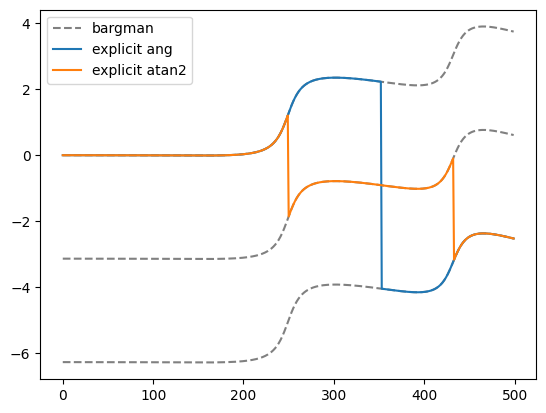
\includegraphics[width = 0.6\textwidth]{fig/premier_resultat}
	\caption[Evolution de la phase géométrique d'un signal AM-FM-PM]{Evolution de la phase géométrique d'un signal AM-FM-PM généré. En gris la phase géométrique du signal calculé via l'invariant de Bargmann. Les deux autres sont calculées avec la formule \cref{eq:phaseg_2var}, en bleu en utilisant de l'argument pour la phase totale et en orange en utilisant atan2.}
\end{figure}

\textbf{\textsc{\color{red} FAIRE LE LIEN AVEC BERRY \cite{berry_quantal_1997} ? plus de détail avec }}
\\

Deux remarques sur ces formules. 
La première est que la phase géométrique ne dépend que des paramètres de polarisations $\theta$ et $\chi$, ce qui reflète son invariance par transformation de jauge.
La seconde, nettement plus troublante, est que $\varphi$ ne s'interprète ni comme phase totale ni comme phase dynamique, un point qui sera expliqué dans la \cref{part:phase_geo}.
\\
Un moyen d'avoir cette interprétation est de supposer qu'à l'instant $t$, $\x $ retrouve la même polarisation instantanée qu'à l'instant $t_0$, auquel cas :
\begin{equation}\label{eq:phases_p-cyc_2var}
	\begin{aligned}
		\big( \chi(t), \theta(t) \big) = \big( \chi(t_0), \theta(t_0) \big)\quad 
		&\Lr\quad \phaset(\x ) = \varphi(t) - \varphi(t) \\
		&\Lr\quad \phaseg(\x ) = -\int_{t_0}^t \theta'(s) \sin 2\chi(s) ds
	\end{aligned}
\end{equation}
\skipl

Même dans ce cas, il est utile de d'avoir une représentation de $\x $ qui soit indépendante de sa phase pour interpréter cette formule \eqref{eq:phases_p-cyc_2var}.
\\



\subsection{Interprétation sur la sphère de Poincaré}\label{subsec:phase_g2Poincare}

Dans l'étude de la phase géométrique, il est standard de s'intéresser à la matrice de covariance\footnote{\itshape
	Il est plus commun en physique de conjuger à droite, mais la conjugaison gauche simplifie l'interprétation de $\rho$ dans la \Cref{fig:sphere2poincare}. Cela est également plus cohérent avec notre définition du produit hermitien qui utilise la convention $\ \langle x, y\rangle = \transp{x}\congu{y}$.
} :
\begin{equation} \label{eq:proj2x_2var}
	\forall t\in\R,\quad \rho_{\x}(t) = \frac{1}{\|\x(t) \|^2} \congu{\x(t) }\, \transp{\x}(t)
\end{equation}
\\
Outre son utilité en traitement du signal, elle présente l'avantage d'être invariante par transformation de de jauge (\ie~ $\rho_{e^{\i \alpha}\x} = \rho_{\x}$).
Aussi c'est matrice sont connue \cite{brosseau} pour avoir pour base les matrices de Pauli $\sigma_i$, ce qui, dans le cas des signaux AM-FM-PM, donne \cite{le_bihan_geometric_2024} :
\begin{equation} \label{eq:decompo_pauli}
	\rho_{\x} = \frac{1}{2}\Big( \Id + \sin(2\theta) \cos(2\chi) \sigma_1 + \sin (2\chi) \sigma_2 + \cos(2\theta) \cos(2\chi) \sigma_3 \Big)
\end{equation}


\begin{wrapfigure}{r}{0.4\textwidth}
	%
\includegraphics[width=0.9\textwidth]{fig/placeholder}
	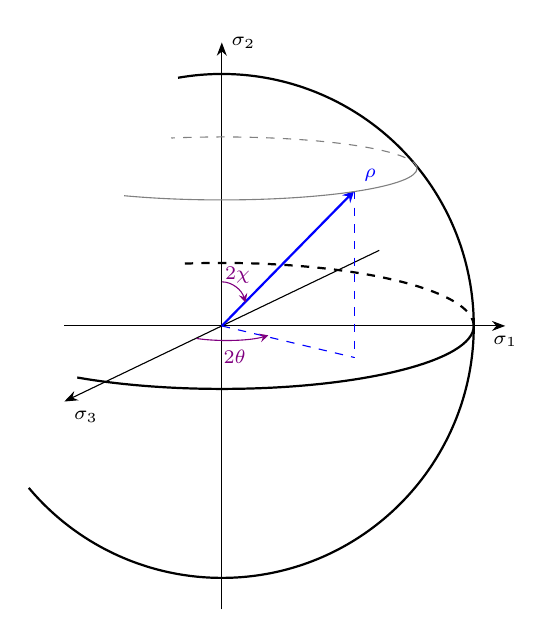
\begin{tikzpicture}[scale=0.8]
	%\draw[black, opacity=0.1] (-4.5,-4.5) grid (4.5,4.5);
	\draw[-Stealth] (-2.5,0) -- (4.5,0) node[below]{$\sigma_1$};
	\draw[-Stealth] (0,-4.5) -- (0,4.5) node[right]{$\sigma_2$};
	\draw[-Stealth] (2.5,1.2) -- (-2.5,-1.2)  node[below right]{$\sigma_3$};
	
	\coordinate (o) at (0,0);
	\coordinate (i) at (4,0);
	\coordinate (j) at (0,4);
	
	\coordinate (u) at (2.1,2.14);
	\coordinate (p) at (2.1, -0.5);
	\coordinate (v) at (3.4,0.5);
	
	% cercles
	\draw[thick] (4,0) arc [start angle=0, end angle =-140, radius = 4];
	\draw[thick] (4,0) arc [start angle=0, end angle =100, radius = 4];
	
	\draw[thick, dashed] (4,0) arc [start angle=0, end angle =100, radius = 4, y radius = 1];
	\draw[thick] (4,0) arc [start angle=0, end angle =-125, x radius = 4, y radius = 1];
	
	% droites
	\draw[-stealth,thick, blue] (0,0) -- (u) node[above right] {$\rho$};
	\draw[dashed, blue] (u) -- (p);
	\draw[dashed, blue] (0,0) -- (p);
	
	%arc au point
	\draw[gray, dashed] (3.1,2.5) arc [start angle=0, end angle =105, radius = 3.1, y radius = 0.5];
	\draw[gray] (3.1,2.5) arc [start angle=0, end angle =-120, x radius = 3.1, y radius = 0.5];
	
	\draw[violet, -stealth] (-0.4, -0.2) arc [start angle=-120, end angle =-40, x radius = 0.9, y radius = 0.225] node[midway, below] {\scriptsize$2\theta$};    
	\draw[violet, -stealth] (0,0.7) arc [start angle=90, end angle =20, x radius = 0.4, y radius = 0.5];
	\draw[violet] (0.25, 0.8) node{\scriptsize$2\chi$};
\end{tikzpicture}
	\caption[\DONE Projection sur la sphère de Poincaré]{Représentation de $\rho_{\x}$ sur la sphère de Poincaré en fonction des paramètres $\theta$ et $\chi$.}
	\label{fig:sphere2poincare}
\end{wrapfigure}

\par \noindent
où les $\sigma_i$ s'écrivent :
\begin{align*}
	\sigma_1 &= \begin{pmatrix} 0 & 1 \\ 1 &  0 \end{pmatrix}  &
	\sigma_2 &= \begin{pmatrix} 0 & -i \\  i &  0 \end{pmatrix}  &
	\sigma_3 &= \begin{pmatrix} 1 & 0 \\ 0 & -1 \end{pmatrix}
\end{align*}
\skipl

Dans cette décomposition, la composante en $\Id$ est indépendante de $\x$ et peut donc être ignorée (idem pour le facteur $\nicefrac{1}{2}$). Cela ne laisse qu'un vecteur (normé) de dimension 3 dont $2\theta$ et $2\chi$ correspondent aux coordonnées sphériques conformément à la \Cref{fig:sphere2poincare} ci-contre.
\\ 
\\
La sphère alors obtenue, plus connue sous le nom de sphère de Poincaré, représente l'ensemble des états de polarisation possibles pour un signal :
\\
À l'équateur, la polarisation est linéaire et $\theta$ pilote son orientation et plus $\rho_{\x}$ se rapproche des pôles, plus cette polarisation devient elliptique, jusqu'à être complètement circulaire, auquel cas $\theta$ devient insignifiant. 
Aussi, suivant le schéma \cref{fig:ellipse2polar}, l'hémisphère nord (resp. sud) correspond à des polarisations elliptiques anti-horaire (resp. horaire).

Le fait que ce soit le double des angles qui sont représentés tient naturellement compte des potentielles redondances dans les $(\theta,\chi)$. 
Par exemple si $\x$ a pour paramètre de polarisation instantanée $(\theta_0, \chi_0)$, alors par symétrie de l'ellipse, $(\theta_0+\pi, \chi_0)$ est aussi une représentation valide. Autre exemple, si $\chi_0 = \nicefrac{\pi}{4}$, alors la polarisation est circulaire et indépendant de $\theta_0$.
\\
Dans les deux cas, la représentation dans la sphère de Poincaré évite ces problèmes puisque, dans le premier cas $(2\theta_0, 2\chi_0)$ et $(2\theta_0+2\pi, 2\chi_0)$ représente le même point, et dans le second, le point associé à $2\chi_0=\nicefrac{\pi}{2}$ (pôle nord) est indépendant du choix de $\theta_0$.

\begin{figure}[H]
	%
\includegraphics[width=0.8\textwidth]{fig/placeholder}
	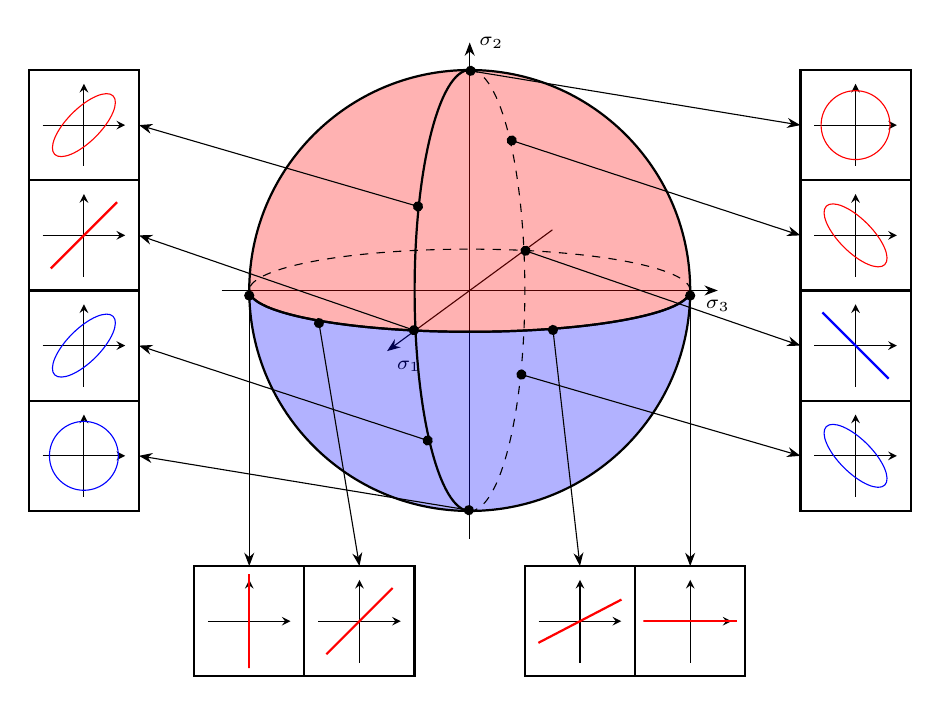
\begin{tikzpicture}[scale=0.7]	
% axes 'n' shit
	%\draw[black, opacity=0.3] (-8.5,-7.5) grid (8.5,5.5);
	\draw[-Stealth] (1.5,1.1) -- (-1.5,-1.1)  node[below right]{$\sigma_1$};
	\draw[-Stealth] (0,-4.5) -- (0,4.5) node[right]{$\sigma_2$};
	\draw[-Stealth] (-4.5,0) -- (4.5,0) node[below]{$\sigma_3$};
	
	\coordinate (o) at (0,0);
	\coordinate (i) at (4,0);
	\coordinate (j) at (0,4);
	
	\coordinate (u) at (2.1,2.14);
	\coordinate (p) at (2.1, -0.5);
	\coordinate (v) at (3.4,0.5);
	
	
% sphère

	% upttom
	\draw[thick, fill=red, fill opacity=0.3] (4,0) arc [start angle=0, end angle =180, radius = 4] --  (-4,0) arc [start angle=-180, end angle =0, x radius = 4, y radius = 0.75];
	
	%bottom
	\draw[thick, fill=blue, fill opacity=0.3] (4,0) arc [start angle=0, end angle =-180, radius = 4]  --  (-4,0) arc [start angle=-180, end angle =0, x radius = 4, y radius = 0.75];
	
	% vertical line
	\draw[thick] (0,4) arc [start angle=90, end angle =270, x radius = 1, y radius = 4];
	
	% back line
	\draw[dashed] (4,0) arc [start angle=0, end angle =180, radius = 4, y radius = 0.75];
	\draw[dashed] (0,4) arc [start angle=90, end angle =-90, x radius = 1, y radius = 4];
	
	
% left boxs

	%frame + axes + ellispe
	\draw[thick] (-8,4) rectangle (-6,-4);
	
	%\draw[thick] (-8,3) -- (-6,3);
	%\draw[-stealth] (-7.75,4) -- (-6.25,4);
	%\draw[stealth-] (-7,4.75) -- (-7,3.25);
	%\draw[color=red, rotate around={45:(-7,4)}] (-6.375,4) arc [start angle=0, end angle =360, radius = 0.625, y radius = 0.625];
	
	
	\draw[thick] (-8,2) -- (-6,2);
	\draw[-stealth] (-7.75,3) -- (-6.25,3);
	\draw[stealth-] (-7,3.75) -- (-7,2.25);
	\draw[color=red, rotate around={45:(-7,3)}] (-6.25,3) arc [start angle=0, end angle =360, radius = 0.75, y radius = 0.3];
	
	\draw[thick] (-8,0) -- (-6,0);
	\draw[-stealth] (-7.75,1) -- (-6.25,1);
	\draw[stealth-] (-7,1.75) -- (-7,0.25);
	\draw[thick, color=red, rotate around={45:(-7,1)}] (-6.15,1) arc [start angle=0, end angle =360, radius = 0.85, y radius = 0];
	
	\draw[thick] (-8,-2) -- (-6,-2);
	\draw[-stealth] (-7.75,-1) -- (-6.25,-1);
	\draw[stealth-] (-7,-0.25) -- (-7,-1.75);
	\draw[color=blue, rotate around={45:(-7,-1)}] (-6.25,-1) arc [start angle=0, end angle =360, radius = 0.75, y radius = 0.3];
	
	
	\draw[-stealth] (-7.75,-3) -- (-6.25,-3);
	\draw[stealth-] (-7,-2.25) -- (-7,-3.75);
	\draw[color=blue, rotate around={45:(-7,-3)}] (-6.375,-3) arc [start angle=0, end angle =360, radius = 0.625, y radius = 0.625];
	
	
% right boxs
	
	%frame + axes + ellispe
	\draw[thick] (8,4) rectangle (6,-4);
	
	\draw[thick] (8,2) -- (6,2);
	\draw[stealth-] (7.75,3) -- (6.25,3);
	\draw[stealth-] (7,3.75) -- (7,2.25);
	\draw[color=red, rotate around={-45:(7,3)}] (7.625,3) arc [start angle=0, end angle =360, radius = 0.625, y radius = 0.625];
	
	\draw[thick] (8,0) -- (6,0);
	\draw[stealth-] (7.75,1) -- (6.25,1);
	\draw[stealth-] (7,1.75) -- (7,0.25);
	\draw[color=red, rotate around={-45:(7,1)}] (7.75,1) arc [start angle=0, end angle =360, radius = 0.75, y radius = 0.3];
	
	\draw[thick] (8,-2) -- (6,-2);
	\draw[stealth-] (7.75,-1) -- (6.25,-1);
	\draw[stealth-] (7,-0.25) -- (7,-1.75);
	\draw[thick, color=blue, rotate around={-45:(7,-1)}] (7.85,-1) arc [start angle=0, end angle =360, radius = 0.85, y radius = 0];
	
	\draw[stealth-] (7.75,-3) -- (6.25,-3);
	\draw[stealth-] (7,-2.25) -- (7,-3.75);
	\draw[color=blue, rotate around={-45:(7,-3)}] (7.75,-3) arc [start angle=0, end angle =360, radius = 0.75, y radius = 0.3];
	
	
	%\draw[stealth-] (7.75,-4) -- (6.25,-4);
	%\draw[stealth-] (7,-3.25) -- (7,-4.75);
	%\draw[color=blue, rotate around={-45:(7,-4)}] (7.625,-4) arc [start angle=0, end angle =360, radius = 0.625, y radius = 0.625];
	
	
	% bottom boxs
	
	%frame + axes + ellispe
	\draw[thick] (-5,-5) rectangle (-1,-7);
	
	\draw[-stealth] (-4.75, -6) -- (-3.25,-6);
	\draw[stealth-] (-4,-5.25) -- (-4,-6.75);
	\draw[thick, color=red, rotate around={90:(-4,-6)}] (-3.15,-6) arc [start angle=0, end angle =360, radius = 0.85, y radius = 0];

	\draw[thick] (-3,-5) -- (-3,-7);	

	\draw[-stealth] (-2.75, -6) -- (-1.25,-6);
	\draw[stealth-] (-2,-5.25) -- (-2,-6.75);
	\draw[thick, color=red, rotate around={45:(-2,-6)}] (-1.15,-6) arc [start angle=0, end angle =360, radius = 0.85, y radius = 0];
	
	
	\draw[thick] (1,-5) rectangle (5,-7);
	
	\draw[-stealth] (1.25, -6) -- (2.75,-6);
	\draw[stealth-] (2,-5.25) -- (2,-6.75);
	\draw[thick, color=red, rotate around={27.5:(2,-6)}] (2.85,-6) arc [start angle=0, end angle =360, radius = 0.85, y radius = 0];
	
	\draw[thick] (3,-5) -- (3,-7);
	
	\draw[-stealth] (3.25, -6) -- (4.75,-6);
	\draw[stealth-] (4,-5.25) -- (4,-6.75);
	\draw[thick, color=red, rotate around={0:(4,-6)}] (4.85,-6) arc [start angle=0, end angle =360, radius = 0.85, y radius = 0];
	
	
% link sphere -- polar
	
	%left
	\draw[thin, {Circle[]}-Stealth] (-0.85,1.5) -- (-6,3);
	\draw[thin, {Circle[]}-Stealth] (-0.925,-0.75) -- (-6,1);
	\draw[thin, {Circle[]}-Stealth] (-0.675,-2.75) -- (-6,-1);
	\draw[thin, {Circle[]}-Stealth] (0.075,-4) -- (-6,-3);
	
	%right
	\draw[thin, {Circle[]}-Stealth] (-0.075,4) -- (6,3);
	\draw[thin, {Circle[]}-Stealth] (0.675,2.75) -- (6,1);
	\draw[thin, {Circle[]}-Stealth] (0.925,0.75) -- (6,-1);
	\draw[thin, {Circle[]}-Stealth] (0.85,-1.5) -- (6,-3);
	
	%bot
	\draw[thin, {Circle[]}-Stealth] (-4,0) -- (-4,-5);
	\draw[thin, {Circle[]}-Stealth] (-2.75,-0.5) -- (-2,-5);
	\draw[thin, {Circle[]}-Stealth] (1.5, -0.625) -- (2,-5);
	\draw[thin, {Circle[]}-Stealth] (4,0) -- (4,-5);

\end{tikzpicture}
	\caption[\DONE États de polarisation associés à divers point de la sphère de Poincaré.]{Représentation des paramètres de polarisation instantanée associés à divers points de la sphère de Poincaré. La couleur donne le sens de parcours de l'ellipse lorsque $\varphi$ varie : en rouge dans le sens trigonométrique et en bleu anti-trigonométrique. Dans les cas de polarisation linéaire, l'orientation n'a pas d'importance.}
	%\\ Dans la colonne de gauche $\theta=\nicefrac{\pi}{4}$ est $\chi$ varie. Idem dans celle de droite avec $\theta=-\nicefrac{\pi}{4}$. En bas, $\chi=0$ et $\theta$ varie.}
\end{figure}


Pour interpréter la formule \eqref{eq:phases_p-cyc_2var} de la phase géométrique prenons un exemple. Si $\chi$ et $\theta$ sont tels que :
\begin{align*}
	\theta(t_0) &= 0  &  \theta(t) &= 2\pi  &  \chi(s) &= \chi_0
\end{align*}
\\
alors $\rho_{\x}$ décrit un chemin horizontal sur la sphère, $\rho_{\x}(t_0) = \rho_{\x}(t)$ et sa phase géométrique s'écrit\footnote{\itshape 
	L'on retrouve dans cette formule le fait que $\phaseg$ est indépendant de la paramétrisation : le résultat est indépendant des l'évolution de $\theta$ sur $]t_0,t[$.} :
\begin{align*}
	\phaseg(\x, t_0, t) = -\int_{t_0}^t \theta'(s) \sin 2\chi(s) ds &= - \sin 2\chi_0 \int_{t_0}^t \theta'(s) ds \\
	&= - \sin 2\chi_0 \big( \theta(t) - \theta(t_0)\big) \\
	&= - 2\pi\sin 2\chi_0
\end{align*}
\skipl

Cette dernière formule donne également, à $2\pi$ près, l’aire de la calotte entourée par $\rho_{\x}$, à savoir :
\[\mathcal{A}ire(\chi_0) = 2\pi - 2\pi \sin(2\chi_0)\]
\\
Pour être précis, pour tenir compte du fait que $\x$ a fait une rotation complète, il est plus naturel de prendre comme phase totale :
\[\phaset(\x) = \varphi(t) - \varphi(t_0) + 2\pi\]
\\
Auquel cas, la phase géométrique donne exactement l'aire de la calotte. Dans la même logique, si l'état de polarisation subit une rotation de $n$ tours, alors $\theta$ va de $0$ à $2n\pi$ et :
\[\phaseg(\x) = 2n\pi - 2n\pi\sin(2\chi_0) = n\mathcal{A}ire(\chi_0)\]
\\
Ainsi, même si $\phaseg$ est définie modulo $2\pi$, le choix du représentant reste important pour mieux tenir compte de l'évolution de $\rho_{\x}$ au court du temps.
\\

En revanche, l'aire totale de la sphère est de $4\pi$, donc l'aire de toute surface de $S^2$ peut être vue comme étant définie modulo $4\pi$, ce qui n'est pas cohérent avec la phase géométrique, qui elle l'est à $2\pi$ près.
\\
Pour résoudre ce problème apparent, il suffit de noter que, tant dis que l’ellipse de polarisation de $\x$ a fait un tour complet, 
$\rho_{\x}$ en a effectué deux sur la sphère ($2\theta(t) = 4\pi$).
Pour qu'il n'en fasse qu'un, il faut faire varier $\theta$ de 0 à $\pi$, auquel cas le terme de la phase géométrique hérité de la $\phaset$ vaut $\pi$ et :
\begin{equation} \label{eq:phase_g2calotte}
	\phaseg(\x, t_0, t) = \pi - \pi\sin 2\chi_0 = \frac{1}{2}\mathcal{A}ire(\chi_0)
\end{equation}
\\
Dans ce cas, la phase géométrique s'interprète comme la demi-aire de la surface entourée par $\rho_{\x}$. Cela n'est, pour l'instant, valable que pour le cas particulier où $\chi$ est constant mais il sera montré dans la \cref{part:phase_geo} que cela se généralise très bien.
\\

Cela étant dit, le fait que $\rho_{\x}$ doive faire deux tours pour que $(\theta,\chi)$ retourne à son état initial, met en évidence un problème quand à la paramétrisations de l'ellipse de polarisation.
\\
Toujours à $\chi$ fixé, si $\theta$ se voit ajouter $\pi$, alors l'état de polarisation est le même, comme expliqué plutôt : $\ \rho(\theta+\pi,\chi) = \rho(\theta, \chi)$.
En revanche, si l'on s'intéresse à un point particulier de l'ellipse, après une rotation de $\pi$, ce même point se retrouvera à l'opposé de là où il était auparavant. 
En d'autre termes, il a subi une rotation de $\pi$ mais qui apparaît non plus dans l'état de polarisation $\rho_{\x}$ mais dans la phase totale (\cref{eq:phase_g2calotte}).
\\
Sachant que $S^2$ est une représentation de rotation $\SO(3)$ de $\R^3$, ce lien entre l'évolution de $\x$ est le nombre de rotations de $\rho_{\x}$ sur $S^2$, n'est pas sans rappeler le fait que $\SU(2)$ est connu pour être un double recouvrement de ce dernier.
\\
\thoughts{Là je dis des conneries, c'est à corriger \href{https://www.youtube.com/watch?v=Ay482u6b3Xo}{avec ca} !!!!}
\\




\subsection{Généralisation en plus haute dimension} \label{subsec:aller_plus_loin}

En résumé. Pour étudier de phase géométrique d'un point de vue signal, il est utile de passer par des notions de paramètres instantanées. Comme l'a montré l'exemple des signaux AM-FM-PM, décomposer un signal en amplitude, phase, et état polarisation donne un cadre propice à la description et l'interprétation de la phase géométrique.
\\

Généraliser cette décomposition en plus haute dimension revient alors à composer $\C^n$ comme un produit de trois ensemble. 
\\
D'abord, en isolant l'amplitude, qui n'est pas très utile à notre propos, $\C^n$ s'écrit :
\[\C^n \cong \R^{+_*} \times S^{2n-1}\]
avec $S^{2n-1}$ la sphère unité de $\C^n$ de dimension réel $2n-1$.
\\
Ensuite, la phase ($e^{\i \varphi}$ dans \eqref{eq:AM-FM-PM}) est un élément de $\U{1}$, donc pour dissocier la phase et état de polarisation, il faudrait décomposer $S^{2n-1}$ de sorte à le faire apparaître. À première vue, il faudrait écrire :
\begin{equation}\label{eq:decompo2C^n}
	\C^n \cong \R^{+_*} \times \U{1} \times \big( S^{2n-1}/\U{1} \big)
\end{equation}
\\
où le quotient qui apparaît n'est autre que l'espace projectif complexe de dimension (complexe) $n-1$ et noté $\PC{n-1}$ (dont la construction sera détaillée dans la \cref{part:phase_geo} suivante).
\\
Le problème de cette formule est qu'elle n'est pas juste en l'état. Plus précisément, elle n'est valable que localement. 
Corrigé cela nécessite d'écrire $S^{2n-1}$, non pas comme un produit de deux ensembles, mais comme un fibré, chose que nous nous attacherons à faire dans la suite de ce mémoire \thoughts{``ce à quoi est dédié la suite de ce mémoire'' serait mieux ?}.
\\

Avant d'y venir et pour motiver d'autant plus la décomposition \eqref{eq:decompo2C^n}, revenons sur le cas $n=2$. Holf a montré, en 1931 \cite{hopf_uber_1931}, que la sphère $S^3$ s'écrit localement (toujours au sens des fibrés) comme le produit $S^1\times S^2$. Le premier étant $\U{1}$ et le second difféomorphe\footnote{\itshape
	Par le premier théorème d'isomorphisme, la projection $\rho$ est équivalente à la projection canonique de $\C^2$ sur $\PC{1}$, de sorte que $\ \rho(\C^n)\cong S^2\cong \PC{1}$.} au plan projectif complexe $\PC{1}$.
Ainsi, l'écriture des signaux AM-FM-PM utilise, sans le dire, la ``décomposition'' \eqref{eq:decompo2C^n}, qui n'est alors qu'une généralisation du modèle utilisé plus tôt.



\part{Aspects Géométriques d'une Phase Éponyme} \label{part:phase_geo} 
Plan approximatif de cette partie :

\begin{enumerate}[label=\Roman* --- ] \bfseries
	
	\item Prérequis \\
	{\normalfont\itshape Dans notre cas, tout s'écrit très simplement donc pas besoin de sortir tout l'arsenal de géo diff}
	\begin{enumerate}[label=\arabic{enumi}.\arabic* --- ]
		
		\item Espace projectif complexe
		\begin{itemize}%[label=\arabic{enumi}.2.\arabic* --- ]
			
			\item Construction de $\PC{n-1}$ 
			\begin{itemize} \normalfont
				
				\item Définition comme espace quotient $\S{2n-1}/\U{1}$
				
				\item $\PC{n}$ vue comme variété différentielle complexe (voir annexe pour détails)
				
				\item \thoughts{lien avec la projection $\x \longmapsto \x\x^\dagger$ utilisé en physique}
				
			\end{itemize}
			
			\item Métrique de Fubini-Study 
			\begin{itemize} \normalfont
				
				\item Métrique induite par la projection
				
				\item expression de la métrique
				
				\item expression en coordonnée local
				
			\end{itemize}
			
		\end{itemize}
		
		\item Fibré principaux
		\begin{itemize}%[label=\arabic{enumi}.1.\arabic* --- ]
			
			\item Fondamentaux
			\begin{itemize} \normalfont
				
				\item Définitions de base
				
				\item Section local (canonique)
				
				\item changement de carte
				
			\end{itemize}
			
			\item Espaces horizontaux et connexion
			\begin{itemize} \normalfont
				
				\item Espace verticaux
				
				\item connexion comme ensemble d'espace horizontaux
				
				\item 1-forme de connexion
				
				\item notre choix de connexion (induite par le produit hermitien)
			\end{itemize}
			
		\end{itemize}
		
	\end{enumerate}
	
	\item Interprétation géométrique des trois phases
	\begin{enumerate}[label=\arabic{enumi}.\arabic* --- ]
		
		\item Cas des signaux ``pseudo-cyclique'' (cyclique à phase près)
 		\begin{itemize} \normalfont
			
			\item Le dessin de Bohm :
			
			\item phase dyn =  signal - horizontal lift
			
			\item phase geo = horizontal lift - cyclique lift (<- indé du signal !)
			
			\item phase tot = cumul des deux
		\end{itemize}
		
		\item La phase géo dans l'espace projectif
		\begin{itemize} \normalfont
			
			\item Géodésique de $\PC{n}$ et généralisation du cas pseudo-cyclique
			
			\item Remarque de Mukunda : phase géo est une 2-forme vs phase dyn est une 1-forme
		
			\item Bonnet-Gauss  \& Stokes : phase géo comme calcul d'air
	
			
			\item \thoughts{Comme partie imaginaire de la métrique \textit{(+ lien avec Fisher)}}
		
		\end{itemize}
	\end{enumerate}
\end{enumerate}
\skipl
\\
\textbf{Annexes}
\begin{enumerate}[label=\Alph* --- ] \bfseries
	
	%\item Forme différentielles \textit{(nécessaire ?)}
	
	\item Algèbre et groupe de Lie
	\begin{itemize}\normalfont
		
		\item def : groupe de Lie $G$
		
		\item def : Algèbre de Lie $\mathfrak{g}$ associée à $G$
		
		\item $\mathfrak{g}$ vu comme tangent $\tg[e]{G}$
		
		\item Cas particulier : $G=\U{1}$
		
	\end{itemize}
	
	\item Variétés différentielles complexe 
	\begin{itemize} \normalfont
		
		\item Complexification de TM
		
		\item L'intérêt de faire ça : proprement définir $\partial/\partial\bar{z}$
		
		\item Exemple : écriture de forme de Kahler de Fubini-Study
		
	\end{itemize}
\end{enumerate}

\newpage


\thoughts{A reprendre, comme toutes les intros} Pour étudier la phase géométrique d'un signal $\psi$, il nous faut projeter $\psi$ sur $\PC{n}$, et ceux, tout en gardant une trace de sa phase puisque c'est le lien entre les deux qui nous intéresse. Il nous faut donc envoyer $\psi$ dans le produit :
\[\U{1}\times \PC{n}\qquad\qquad (\text{ou }\ \C^{n-1*}/\C^*)\]
\\
Garder le lien entre cet espace et celui d'origine mène à se placer dans le cadre avec d'un \emph{variété fibrée} (ou simplement fibré). Plus précisément, comme $\U{1}$ est un groupe de lie, ce sera un \emph{fibré principal} noté $\S{2n+1}\big(\U{1},\PC{n}\big)$.
\\

Comme son nom l'indique, $\S{2n+1}\big(\U{1},\PC{n}\big)$ à une structure de variété différentielle et le lien entre les $\U{1}$ et $\PC{n}$ va se faire par le biais d'une connexion. L'on verra alors que cette connexion est intrinsèquement lié à la phase dynamique du signal, et il sera discuté de la signification de ce résultat.
\\
La phase géométrique, quand à elle, sera liée avec la métrique hermitienne associée aux l'espaces projectifs complexes.
\\
Tout cela va demander quelques prérequis que nous allons voir à présent.
\\



\section{Prérequis mathématique}

\subsection{Variétés différentielles complexes et les espaces projectifs complexes}\label{subsec:PC^n}

Les espaces projectifs complexes se construisent ainsi. On se place dans ${\C^{n+1}}^*=\C^{n+1}\setminus\{0_{\C^{n+1}}\}$ avec la relation d'équivalence, $\forall x,y\in{\C^{n+1}}^*$ :
\[x \sim y\ \Llr\ \exists \lambda\in\C^*\ |\ x=\lambda y\]
\\
L'espace projectif complexe, noté $\PC{n}$, est l'espace quotient :
\[\PC{n} = {\C^{n+1}}^*/\C^* = {\C^{n+1}}^*/\sim\]
\\
En notant $[z]$ la classe de $\PC{n}$ du représentant $z = (z^i)_{0\leq i\leq n}\in{\C^{n+1}}^*$, on définit les ensembles et cartes, $\forall i\in\llbracket0,n\rrbracket$ :
\begin{align}
	U_i &= \Big\{[z]\in\PC{n}\ \big|\ z^i\neq 0\Big\}  &  \phi_i\  :\quad &\begin{aligned}
		U_i\ \ &\lr\quad\ \C^{i}\times \{1\} \times\C^{n-i}\cong \C^{n} \\ [z]\ \ &\lmt\ \frac{1}{z^i}\big(z^0,\cdots, z^i,\cdots, z^n\big)
	\end{aligned}
\end{align}
\\
L'ensemble d'arrivé $\phi_i(U_i)$ est de dimension $n$ et s'assimile à $\C^{n}$ mais, par souci de comodité, on restera dans $\C^{n+1}$. Cela permet  d'écrire plus simplement les formules de changement de carte en évitant de devoir enlever et rajouter des coefficients :
\[ \forall [z]\in U_i\cap U_j\quad (\ie~z^{i,j}\neq 0) ,\qquad \phi_i \circ {\phi_j}^{-1}(z) = \frac{z^j}{z^i}z\]

Les $(U_i,\phi_i)$ forment ainsi un atlas holomorphe sur l'espace projectif complexe, faisant de $\PC{n}$ une variété complexe de dimension $\dim[\C] = n$ (voir annexe \ref{ann:variet_complexe} pour plus de détail).


\begin{proposition}
	$\PC{n}$ admet une métrique hermitienne induite par la métrique de $\S{2n+1}$, elle même induite du produit scalaire sur $\R^{2n+1}$. Elle est appelé \emph{métrique de Fubini-Study} et est donnée par le formule :
	\[\]
\end{proposition}
\skipl



\subsection{Variété fibrée principale et connexion} \label{subsec:VFP}

Pour le dire simplement, les \emph{variétés fibrés} sont des variétés qui ressemble localement à des espaces produits. 
Le ruban de Modiüs en est un exemple typique : il ne peut pas s'écrire comme le produit d'un cercle avec un segment $\S{1}\times [0,1]$ à cause de la façon dont il est construit. Mais localement, il est tout à fait comparable (\ie~difféomorphe) à un tel produit (\cf~\cref{fig:ruban2modius}).
\\

Il existe toutes sorte de variétés fibrées dès lors qu'elles sont munies de structure remarquable. Celles qui vont nous intéresser sont les variétés fibrées dites principales\footnote{\itshape
	Bien que ce ne sera pas précisé, il sera toujours sous-entendu que les différentes variétés et cartes doivent avoir les mêmes niveaux de régularités pour que le tout reste cohérent.} :
\\
\begin{definition}[Variété fibrée principale] \label{def:VFP}
	Une \emph{variété fibrée principale}(VFP), ou \emph{fibré principal} est constituée de deux variétés différentielles $P$ et $B$ telles que :
	\begin{itemize}
		\item Il existe un groupe de Lie $G$ opérant à droite (ou à gauche) sur $P$ via l'application différentiable :
		\begin{equation} \label{eq:VFP_action}
			R\ :\ \begin{aligned}P\times G\ &\lr\quad\ \ P \\ (p,g)\ \ &\lmt\ R_g(p)\defeq p\cdot g = pg
			\end{aligned}
		\end{equation}
		
		\item Il existe une surjection différentiable $\ \pi:P\lr B\ $ telle que :
		\begin{equation} \label{eq:VFP_fibres}
			\forall p\in P,\quad \pi^{-1}\big(\pi(p)\big)=pG
		\end{equation}
		
		\item $P$ est munie d'un ensemble de paire $(U_i, h_i)$ tel que les $U_i$ forment un recouvrement de $B$ et tel que les $h_i : G\times U_i\lr \pi^{-1}(U_i)\subset P$ soient des difféomorphismes vérifiant :
		\begin{align*} \label{eq:VFP_atlas}
			\forall a,b\in G,\ \forall x\in B,\qquad h_i(ab,x) = h_i(a,x) \cdot b\qquad \text{et} \qquad \pi\circ h_i(a,x) = x
		\end{align*}
	\end{itemize}
	
	\begin{adjustbox}{valign=C,raise=1cm, minipage={1.1\linewidth}}
		\begin{wrapfigure}{r}{0.35\textwidth}
			\begin{tikzcd}[column sep=large]
				G\times U_i \arrow[d, "\pr{2}" left]  \arrow[r, "h" above]  & \pi^{-1}(U_i) \subset P \arrow[ld, "\pi" below right] \\
				U_i
			\end{tikzcd}
			%\caption{Digramme sûrement osef des jeux de projections entre $P$ et les cartes locales}
			\label{diagram_commu_VFP}
		\end{wrapfigure} 
		\vspace*{-0.5cm} % This is a fudge to align the top of the theorem environment with the image
		\skipl\par 
		La variété $B$ est appelé la \emph{base} de la VFP, que $G$ son \emph{groupe structural} et $pG$ la \emph{fibre de $P$ passant par} $p$ et \emph{au dessus de} $\pi(p)\in B$. Le tout est notée $P(R, G, \pi, B)$ ou plus simplement $P(G,B)$.
		
		Les fibres $pG$ sont toutes difféomorphes à $G$ et $B$ est difféomorphe à $P/G$. \thoughts{Le diagramme commutatif ci-contre résume la situation.}
	\end{adjustbox}
\end{definition}
\skipl 
\begin{figure}[h]
	
\includegraphics[width=0.45\textwidth]{fig/placeholder}
	%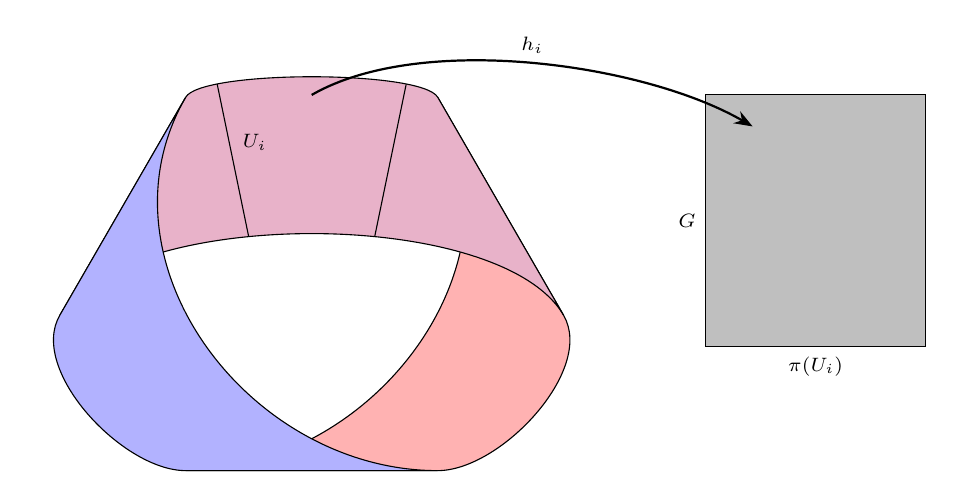
\begin{tikzpicture}[scale=0.8]
	%\draw[opacity=0.1] (-4.5,-4.5) grid (12.5,4.5);
	
	
%%%%     MOBIUS     %%%%

	%main points
	\coordinate (s1-) at ($(90+0-30:4) + (0,-1)$);
	\coordinate (s1+) at ($(90+0+30:4) + (0,-1)$);
	
	\coordinate (s2+) at ($(90+120-30:4) + (0,-1)$);
	\coordinate (s2-) at ($(90-120+30:4) + (0,-1)$);
	
	\coordinate (s3+) at (90+120+30:4);
	\coordinate (s3-) at (90-120-30:4);
	
	%\draw (s1-) -- (s2+) -- (s3-) -- (s1-);
	%\draw (s1+) -- (s3+) -- (s2-) -- (s1+);
	%\draw (s3+) -- (s3-);
	\colorlet{tmpb}{blue!30!};
	\colorlet{tmpr}{red!30!};
	\colorlet{tmpv}{blue!30!red!30!};
	\definecolor{tmpg}{gray}{0.75};
	
	
	% bande droite
	\draw[fill=tmpr] (s1-) .. controls  ($(s1-)+(-60:3)$) and  ($(s3+)+(0:3)$) .. 
		(s3+) -- (s3-) 
		.. controls ($(s3-)+(0:1)$) and ($(s2-)+(-60:1)$) .. 
		(s2-) -- cycle;
		
	% bande haut
	\draw[fill=tmpv] (s1-) .. controls  ($(s1-)+(120:0.5)$) and  ($(s1+)+(60:0.5)$) .. 
		(s1+) -- (s2+) 
		.. controls ($(s2+)+(60:2)$) and ($(s2-)+(120:2)$) .. 
		(s2-) -- cycle;
		
	% bande gauche
	\draw[fill=tmpb] (s1+) .. controls  ($(s1+)+(-120:3)$) and  	($(s3-)+(-180:3)$) .. 
		(s3-) -- (s3+) 
		.. controls ($(s3+)+(-180:1)$) and ($(s2+)+(-120:1)$) .. 
		(s2+) -- cycle;
		
		
	%%%%     CARTE LOCALE     %%%%
	
	% ouvert U_i
	\draw (-1,0.25) -- (-1.5,2.67) node[midway, above right]{$U_i$};
	\draw (1,0.25) -- (1.5,2.67);
	
	% carte
	\draw[fill=tmpg, shift={(6.25,-1.5)}] (0,0) -- (0, 4) node[midway, left]{$G$} -- (3.5,4) -- (3.5,0) -- cycle node[midway, below]{$\pi(U_i)$};
	
	% fleche vers la carte
	\draw[-Stealth, thick] (0,2.5) ..
	controls ($(0,2.5) + (30:2)$)  and ($(7, 2) + (180-30:2)$) .. (7, 2) node[midway, above]{$h_i$};
	
\end{tikzpicture}
	\caption[Ruban de Mobius comme variété fibrée]{Représentation du ruban de Modius en tant que fibré. Même s'il n'est pas principale, les notations sont reprise de la \cref{def:VFP}.}
	\label{fig:ruban2modius}
\end{figure}


L'ensemble $\big\{(U_i, h_i)\big\}_i$ est l'équivalent d'un atlas pour les variétés différentielles classiques mais adapter pour tenir compte de la structure fibré de $P$ et de l'action de $G$. Explicité les changements de cartes dans $P$, ce fait comme suit.
\\
D'abord, $P$ étant localement difféomorphe à un produit $G\times U_i$, on peut y tracer des graphes appelés \emph{sections locales}, comme sur la \Cref{fig:section_local} \thoughts{ci-dessous}. Formellement, une section locale au dessus  de $U_i \subset B$ est une application $\sigma : U_i \lr P$ vérifiant :
\[\pi\circ \sigma = id_{{\displaystyle |}U_i}\]
\begin{figure}[H]
	\begin{floatrow}
		\ffigbox{\caption[Représentation d'une section local]
			{Représentation d'une section local $\sigma$ au dessus de $U_i$. Comme $P$ n'est pas un produit à proprement parler, $\sigma$ est représenté dans $G\times U_i$ à travers $h_i$.}
			\label{fig:section_local}}{
		%
\includegraphics[width=0.45\textwidth]{fig/placeholder}
		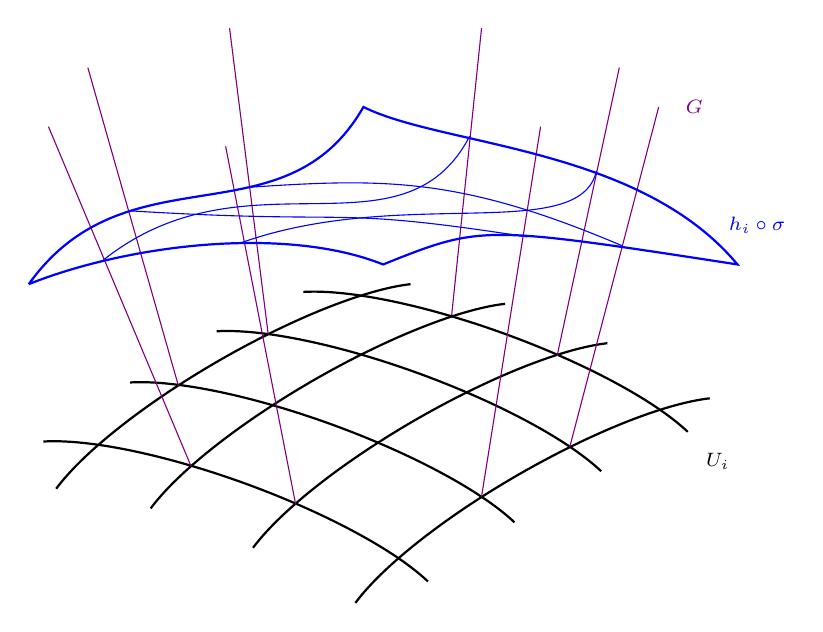
\begin{tikzpicture}%[scale=0.9]
	%\draw[opacity=0.1] (-4.5,-4.5) grid (4.5,4.5);

	%\draw (-1,-4)  .. controls (0,-2.5) and (1.5,-1.75) ..  (4,-2);

% BASE

	% gauche
	\draw[thick, xshift=1.3cm, yshift=-3.2cm, rotate=30]
		(3,0) arc [start angle=30, end angle =150, radius = 3, y radius = 0.75];
		
	\draw[thick, xshift=0cm, yshift=-2.5cm, rotate=30]
		(3,0) arc [start angle=30, end angle =150, radius = 3, y radius = 0.75];
		
	\draw[thick, xshift=-1.3cm, yshift=-2cm, rotate=30]
		(3,0) arc [start angle=30, end angle =150, radius = 3, y radius = 0.75];
		
	\draw[thick, xshift=-2.5cm, yshift=-1.75cm, rotate=30]
		(3,0) arc [start angle=30, end angle =150, radius = 3, y radius = 0.75];
		
	% droite
	\draw[thick, xshift=-2.5cm, yshift=-3cm, rotate=-20]
		(3,0) arc [start angle=30, end angle =150, radius = 3, y radius = 0.75];
	
	\draw[thick, xshift=-1.4cm, yshift=-2.25cm, rotate=-20]
		(3,0) arc [start angle=30, end angle =150, radius = 3, y radius = 0.75];
	
	\draw[thick, xshift=-0.3cm, yshift=-1.6cm, rotate=-20]
		(3,0) arc [start angle=30, end angle =150, radius = 3, y radius = 0.75];
	
	\draw[thick, xshift=0.8cm, yshift=-1.1cm, rotate=-20]
		(3,0) arc [start angle=30, end angle =150, radius = 3, y radius = 0.75];
	
	
% FIBRES

	\draw[violet] (-1.36,-3.05) -- (-2.25,1.5);
	\draw[violet] (1,-2.95) -- (1.75,1.75);
	
	\draw[violet] (-2.69,-2.56) -- (-4.5,1.75);
	\draw[violet] (2.12,-2.32) -- (3.25,2);
	
	\draw[violet] (-2.85,-1.54) -- (-4,2.5);
	\draw[violet] (1.96,-1.16) -- (2.75,2.5);
	
	\draw[violet] (-1.71,-0.88) -- (-2.2,3);
	\draw[violet] (0.62,-0.65) -- (1,3);
	
	
% SECTION

	%frame
	\draw[thick, blue] (-4.75,-0.25) .. controls (-3.5,1.5) and (-1.5,0.25) ..  
		(-0.5,2) .. controls (0.5,1.5) and (3,1.5) ..
		(4.25,0) .. controls (1,0.5) ..
		(-0.25,0) .. controls (-1.5,0.5) and (-3.5,0.25) ..
		(-4.75,-0.25);
		
	% coordo droite
	\draw[blue] (-3.45,0.68) .. controls (-0.5,0.5) and (-1,0.75) .. (1.58,0.35);
	\draw[blue] (-1.95,0.98) .. controls (-0.2,1.1) and (0.75,1.1) .. (2.78,0.24);
	
	%coordo gauche
	\draw[blue] (-3.81,0.05) .. controls (-2,1.5) and (0,0) .. (0.85,1.63);
	\draw[blue] (-2.04,0.28) .. controls (0,1) and (2.25,0.25) .. (2.46,1.19);
	
% NOTATION
	\draw (4,-2.5) node{ $U_i$};
	\draw (3.7,2) node{\color{violet} $G$};
	\draw (4.5,0.5) node{\color{blue} $h_i \circ \sigma$};
	
\end{tikzpicture}}
	
	\ffigbox{\caption[Représentation de la section canonique]
		{Représentation de la section canonique définie par rapport à $G$.}}{
		
\includegraphics[width=0.45\textwidth]{fig/placeholder}
		\label{fig:section_cano}}
\end{floatrow}
\end{figure}
\noindent
Ensuite, les hypothèses sur $P(G,B)$ sont telles que $G$ agit transitivement et librement (ou sans point fixe) sur $P$. C'est-à-dire que, sur une même fibre, tout point peut être atteint par n'importe quel autre via l'action de $G$ (transitivité) :
\begin{align*}
	\forall x\in B,\quad \forall p,q\in P_x,\ \exists t(p,q)\in G\ |\ p = q\cdot t(p,q) 
\end{align*}
et que la seule façon de laisse les points invariants par cette même action est de passer par l'élément neutre $e$ (libre) :
\begin{align*}
	\forall (p,g)\in P\times G,\quad p = p\cdot g\ \Lr\ g=e
\end{align*}
\\
De la transitivité de $G$, découle le fait que toutes les sections locales $\sigma$ au dessus de $U_i$ peuvent s'écrire à partir d'une même section $\sigma_i$ via la formule :
\[\forall x\in B,\qquad \sigma(x) = \sigma_i(x) \cdot t\big(\sigma_i(x), \sigma(x)\big)\]
Son caractère libre, lui assure l'unicité d'un choix canonique de section $\sigma_i$ sur $U_i$. Elle est donnée par :
\[{h_i}(x,e) = \sigma_i(x)\]
Cela mène à la définition :
\begin{definition}[Fonctions de transitions]
	L'intersection de deux cartes  est noté $U_{ij} = U_i\cap U_j$ et le passage d'une section local canonique est donné par :
	\[\forall x\in U_{ij},\qquad \sigma_j(x) = \sigma_i(x) t\big(\sigma_i(x), \sigma_j(x)\big)\]
	L'élément de $G$, $t(\sigma_i, \sigma_j)$, est alors appelé \emph{fonction de transition} et sera noté $\varphi_{ij}$. Elle fait effectivement la transition entre deux cartes dans le sens où :
	\[\forall (g,x)\in G\times U_{ij},\qquad {h_i}^{-1} \circ h_j(g,x) = \big( \varphi_{ij}(x)g, x \big)\]
\end{definition}
\skipl

Dans la suite, il sera nécessaire de munir $P$ d'une connexion, qui s'introduit comme suit.
\\
Comme $P$ ressemble localement à un produit $G\times U_i$, il est utile de séparer ses espaces tangents $\tg[p]{P}$ comme une somme directe d'espaces tangents respectivement aux fibres et à la base. Conformément aux représentations précédentes (\cref{fig:ruban2modius,fig:section_cano,fig:section_local}), les premiers sont appelées espaces tangents \emph{verticaux}, les seconds \emph{horizontaux} et l'on note :
\[\forall p\in P,\qquad \tg[p]{P} = \vg[p]{P} \oplus \hg[p]{P}\]
\\
Les tangents verticaux $\vg[p]{P}$ se définissent canoniquement par rapport à $\pi$. Pour cela, la \emph{fonction tangente} (ou \emph{dérivée}) \emph{de $\pi$ au point} $p$ est noté $\tg[p]{\pi}$ avec :
\[(\tg[p]{\pi})^i_j = \frac{\partial \pi^i}{\partial x^j}(p) = \partial_j\pi^i(p)\]
\\
Ainsi, $\tg[p]{\pi}$ est à valeur de $\tg[p]{P}$ dans $\tg[\pi(p)]{B}$ et l'espace tangent vertical au point $p$ se défini comme :
\[\vg[p]{P} \defeq \Ker (\tg[p]{\pi}) = \big\{ v\in\tg[p]{P}\ |\ \tg[p]{\pi}(v)=0 \big\}\]
\\ 
Il s'avère que les espaces horizontaux ne peuvent pas être construit de cette façon. Il faut donc faire un choix pour les $\hg[p]{P}$ et c'est ce choix qui est appelé connexion (elle connecte les esapce tangents entre eux).
Ces sous-espaces peuvent être caractérisé par une 1-forme différentiable $\conn$ sur $P$ à valeur dans $\vg[p]{P}$, auquel cas :
\[\forall p\in P,\quad \hg[p]{P} = \Ker(\conn_p)\]
\skipl

Dans le cas des VFP, une connexion --- et sa 1-forme --- doit en plus avoir de bonnes propriétés au regarde de l'action $R$, aboutissant à la définition :
\begin{definition}[Connexion sur VFP] \label{def:connexion2VFP}
	Une \emph{connexion} sur une VFP $P(G,B)$ est la donnée d'un sous-espace tangent, $\hg[p]{P}\subset \tg[p]{P}$, en tout point de $p\in P$ tel que :
	\begin{itemize}
		
		\item $\hg{P}$ dépend différentiellement de $p$ (``dépendre différentiellement'' à un sens précis mais qui ne sera pas utile pour la suite).
		
		\item $\hg[p]{P}$ est supplémentaire à $\vg[p]{P}$ dans $\tg[p]{P}$ :
		\begin{equation}\label{eq:TP=V+H}
			\tg[p]{P} = \vg[p]{P} \oplus \hg[p]{P}
		\end{equation}
		
		\item l'assignation des $\hg[p]{P}$ est invariantes pas l'action de $G$ au sens où :
		\begin{equation}\label{eq:conn_G-inv}
			\forall (p,g)\in P\times G,\quad \tg[p]{R_g} (\hg[p]{P}) = \big\{\tg[p]{R_g}(v)\ |\ v \in \hg[p]{P} \big\} = \hg[R_g(p)]{P}
		\end{equation}
		
	\end{itemize}
	
	Comme les fibres de $P$ sont toutes de la forme $pG$, les espaces $\vg[p]{P}$ s'identifient aux espaces tangents à $G$, qui eux-même s'identifie à l'algèbre de Lie $\mathfrak{g}\cong \tg[e]{G}$ de $G$. Ainsi, dans le cas des VFP, la \emph{1-forme de connexion} $\conn$ est une 1-forme différentiable sur $P$ à valeur dans $\mathfrak{g}$ (\ie~en tout point $p\in P$, $\conn_p$ est valeur de $\tg[p]{P}$ dans $\mathfrak{g}$), auquel cas on a toujours :
	\begin{equation} \label{eq:1-form2conn}
		\forall p\in P,\quad \hg[p]{P} \defeq \Ker(\conn_p)
	\end{equation}
	\skipl
	
	Enfin, $\conn$ induit une 1-forme sur les cartes $U_i$ via la section canonique $\sigma_i$. Elle est noté $\locconn_{i}$ et pour que les $\locconn_i$ induisent une connexion sur $P$ il faut et il suffit que sur le chevauchement $U_{ij}$, $\locconn$ se transforme suivant :
	\begin{equation}\label{eq:conn_local}
		\locconn_j = {\varphi_{ij}}^{-1} \locconn_i \varphi_{ij} + {\varphi_{ij}}^{-1} \d \varphi_{ij}
	\end{equation}
\end{definition}
\skipl




\section{Interprétation des trois phases dans ce cadre}

\subsection{HHHHH}

blablabla maintenant on peut recoller les morceaux.
 
Comme $\PC{n}$ est une variété quotient, elle induit naturellement une variété principale :
\begin{proposition}
	La $2n+1$--sphère $\S{2n+1}$, vu comme variété plongée dans $\C^n$ est une VFP de base $\PC{n}$ et de fibre type $\U{1}$. L'action de $\U{1}$ sur $\S{2n+1}$ étant induite par le produit complexe classique et où :
	\begin{itemize}
		\item La fibration $\pi$ est la projection canonique de $\S{2n+1}$ sur $\PC{n}$ :
		\[\pi\ :\ \begin{aligned}\S{2n+1}\ &\lr\ \PC{n} \\ x\quad\ &\lmt\ \ [x]\end{aligned}\]
	
	\item Les cartes locales $h_i$ sont telles que :
	\[\forall z \in \pi^{-1}(U_i),\  {h_i}^{-1}(z) = \big( z_i/|z_i|, [z] \big)\in \U{1} \times \PC{n}\]
	
	\item Tout les représentant $z$ d'un élément de la base $\zeta\in\PC{n}$ sont normé, ainsi, alors tout La section canonique au dessus des $U_i$, $\sigma_i$ elle est définie par :
	\[\]
	
	\end{itemize}
	
	Voir \cite[lemme 2.17]{lafontaine_introduction_2015} pour une démonstration de l'aspect fibré.
\end{proposition}
\subsection{Cas pseudo-cyclique}





%%%% ANNEXES %%%%



\begin{annexe}

\section{Annexe}

\subsection{Connexion induite par une métrique}

Si $P(G,B)$ une VFP munie d'une métrique riemannienne $g$. La connexion induite par $g$ sur $P$ est définie par :
\begin{equation}
	\forall p\in P,\quad \hg[p]{P} = \vg[p]{P}^\perp
\end{equation}
\\
Plus concrètement, $\vg[p]{P}$ est isomorphe à $\mathfrak{g}$ via la transformation :
\[\forall p\in P,\ \forall a\in\mathfrak{g},\quad a^*(p) = \frac{d}{dt} p\cdot \exp(t a)\big|_{t=0} = \frac{d}{dt} p\cdot \exp(t a)\big|_{t=0}\defeq pa\]
\\
Avec, une base $\{\mathfrak{e}_i\}_{1\leq i\leq k}$ de $\mathfrak{g}$ induit un base $\{e_i\}_{1\leq i\leq k} = \{\mathfrak{e}^*_i\}_{1\leq i\leq k}$ sur $\vg[p]{P}$. La métrique $g$ induit alors une connexion de 1-forme :
\[\conn_g(X) = \sum_i g(X, e_i) \mathfrak{e}_i = \sum_i g_{ij}X^j \mathfrak{e}_i\]
\\
et on la projection de $X$ sur $\vg{P}$ est donnée par :
\begin{align*}
	\ver X = \conn(X)^*\quad &\Llr\quad  \ver (X^ie_i) = \sum_i g_{ij}X^j e_i \\
	&\Llr\quad  (\ver X)^i = g_{ij}X^j
\end{align*}


\subsection{Algèbre et groupe de Lie} \label{ann:2Lie}




\subsection{Variété différentielle complexe, tiré de \cite{nakahara_geometry_2003}}

Pour mémoire, une variété différentielle de classe $C^k$ ($k\in\N\cup\{\infty\}$) de dimension $n$ est un espace topologique\footnote{\itshape
	La topologie de $\manu$ doit vérifier des propriétés type séparable, dénombrable à l'infinie, \etc, qui seront toutes admises dans la suite, voir par exemple \cite[chap. 2]{lafontaine_introduction_2015}}
$\manu$ (ou $\manu^n$) munie d'un \emph{atlas} $(\phi_i, U_i)_{i\in I}$, c'est-à-dire un ensemble finie de pair d'ouvert $U_i\subset \manu$ et d'application $\phi_i :U_i\ \lr\ \R^n$ telle que :
\begin{itemize}
	
	\item les $U_i$ forme un recouvrement de la variété :\qquad $\bigcup_{i\in I} \phi_i(U_i) = \manu$
	
	\item les $\phi_i$ sont des homéomorphismes sur leur image $\phi_i(U_i)\subset\R^4$.
	
	\item si l'intersection $U_i \cap U_j$ est non vide, alors ${\phi_j \circ {\phi_i}^{-1}}_{| {\phi_i}^{-1}(U_i\cap U_j)}$ est un $C^k$ difféomorphisme sur son image.
\end{itemize}

$\manu$ sera une \emph{variété différentielle complexe} si elle satisfait les propriétés ci-dessus où $\R^n$ est remplacé par $\C^n$ et où la condition de difféomorphisme est remplacé par la condition d'holomorphisme. 
\\
Une application $f : \C^n\lr \C^n$ étant holomorphe si chacune de ses composantes vérifie l'équation de Cauchy-Riemann :
\[\forall x,y\in\R^n,\ \forall \mu,\qquad \frac{\partial f }{\partial y^\mu}(x+iy) = i \frac{\partial f }{\partial x^\mu}(x+iy)\]
\\
Les fonctions holomorphes étant automatiquement $C^\infty$, les variétés différentielles complexes sont toujours lisse, c'est-à-dire $C^\infty$. Aussi, $\manu$ est dite de dimension complexe $n$ et dimension (réel) $2n$, notés :
\begin{align}\label{eq:manuC-base_cano}
	\dim[\C](\manu) &\defeq n  &  \dim[\R] (\manu) \defeq \dim (\manu) = 2n
\end{align}
\\

Ensuite, pour le dire rapidement, la structure complexe de $\manu$ permet de séparer les espaces tangents en deux sous espaces. Pour ce faire, on commence par noter qu'en tout point $p\in\manu$ de coordonnée $z^\nu=x^\nu+iy^\nu$, l'espace tangent $\tg[p]{\manu}$, vu comme variété réelle, admet une base :
\begin{equation}
	\tg[p]{\manu} = \vec \left\{ \frac{\partial}{\partial x^1}, \cdots, \frac{\partial}{\partial x^n}, \frac{\partial}{\partial y^1}, \cdots,  \frac{\partial}{\partial y^n} \right\}
\end{equation}
\\
Plus tôt que de se basé sur les $x^\mu$ et $y^\mu$ pour séparer les $\tg[p]{\manu}$, on définit sur ces derniers un tenseur $J_p$ de type (1,1) tel que :
\begin{align}
	J_p \frac{\partial}{\partial x^\mu} &= \frac{\partial}{\partial y^\mu}  &  J_p \frac{\partial}{\partial y^\mu} &= -\frac{\partial}{\partial x^\mu}
\end{align}
\\
Ce tenseur est l'équivalent de la multiplication par $\pm i$ et le fait que $\manu$ soit complexe assure qu'il soit défini globalement, \ie~sur $\tg{\manu}$. Il est diagonaliseable dans la base :
\begin{align}\label{eq:manuC-base_holo}
	\partial_\mu = \frac{\partial}{\partial z^\mu} &\defeq \frac{1}{2}\left( \frac{\partial}{\partial x^\mu} - i\frac{\partial}{\partial y^\mu} \right)  
	&  
	\partial_{\bar{\mu}} = \frac{\partial}{\partial \overline{z}^\mu} &\defeq \frac{1}{2}\left( \frac{\partial}{\partial x^\mu} + i\frac{\partial}{\partial y^\mu} \right)
\end{align}
\\
Ainsi en fonction de la base (\eqref{eq:manuC-base_cano} ou \eqref{eq:manuC-base_holo}), $J_p$ va s'écrire :
\begin{align}
	J_p &= \begin{pmatrix}
		\text{\large\ 0\ }\Big. & I_n \\ -I_n & \text{\large\ 0\ }\Big.
	\end{pmatrix}  &
	J_p &= \begin{pmatrix}
		iI_n & \text{\large\ 0\ }\Big. \\ \text{\large\ 0\ }\Big. & -iI_n
	\end{pmatrix} 
\end{align}
\\
Finalement, $\tg{\manu}$ peut être séparé en deux sous-espaces engendré respectivement par les $\partial_\mu$ et $\partial_{\bar{\nu}}$. On parle de vecteur holomorphe et anti-holomorphe et on note :
\begin{align}
	\tg[p]{\manu}^+ &= \Vec\big\{ \partial_\mu\ |\ 1\leq \mu\leq n \big\}  &  \tg[p]{\manu}^- &= \Vec\big\{ \partial_{\bar{\mu}}\ |\ 1\leq \mu\leq n \big\}
\end{align}

\end{annexe}





\part{\todo Applications et généralisation} \label{part:app&gene} 

\section{Calcul pratique de la phase géométrique}

\subsection{Invariant de Bargmann}

\begin{itemize}
	\item L'idée c'est d'approcher la courbe par des géodésiques
	
	\item géodésique $\Lr\ \phaseg = \phaset$ donc c'est juste des arg !
	
	\item En cumulant le tout, ca fait donne l'invariant de Bargmann :
	
	\item Bonus : c'est super parce que, en pratique, on a toujours des données ponctuelles, dont pas de besoin de "choisir" la subtivision !
\end{itemize}



\subsection{Lien avec la première partie}

\begin{itemize}
	\item La présentation dans $\PC{n}$ à été fructueuse dimension (complexe) $n=1$, avec les paramètres de l'ellipse. Mais, au delà, ca devient moins clair. Intuitivement, on pourrait généraliser les états de polarisations en ajoutant simplement une matrice de rotation dans $\C^n$ au signal bivarié polarisé. Autrement dit, il faudrait découper $\PC{n}$ en une produit du genre :
	\[\PC{n} \cong \SO_n(\R)\times \PC{2}-ish\]
	C'est pas clair comment faire ça (est-ce que $\SU_n(\C)$ serait mieux ?)
\end{itemize}



\section{Application}

\subsection{Information apportée}

\begin{itemize}
	\item Si une source d'information n'est pas sensé changer d'état de polarisation, mais qu'on constate qu'il y a phase géométrique, alors ce n'est (quasiment) que du bruit. Ça peut donc être un premier filtre pour débruiter.
	\\
	
	Pour le corriger en revanche, c'est un peu plus technique parce que ça veut dire qu'il faut faut TUER la polarisation du signal.
	\\
	Une idée serait de regarder la moyenne du signal projeté dans $\PC{n}$ et du tout simplement remplacer l'état de polarisation du ce signal par ca moyenne.
	
	\item En étant un peu moins restrictif l'évolution de l'état de polarisation du signal, on a vu qu'un la phase instantanée doit contenir les hautes fréquences du signal, Peut-être qu'on pourrait se servir de ça pour contraindre les variations de l'état de polar et, là encore, en faire un critère de débruitage. Genre tué les hautes fréquences de la phase géométrique
	
	\item D'ailleurs, ca amène la question : QUIDE de faire du Fourier sur les phases ? La phase totale est pas très intéressante, mais les deux autres, elle sont, en gros à valeur dans $\R$.\\
	Donc qu'est-ce qu'on peut dire de $\Fou{\phaseg}$ ? est-ce qu'on peut en faire des trucs (passe-bas notamment).
	
\end{itemize}




\subsection{Sensibilité de la phase géométrique par rapport au bruit}

\begin{itemize}
	\item Il faudrait voir comment la phase géométrique réagit au bruit.
	
	\item Si elle y est très résiliente, elle pourrait être source d'information sur des données. Voir même, être une information de base pour reconstruire une signal (genre en utilisant le fait qu'elle soit à propos des basse-fréquence)
	
	\item Plus généralement, il serait bien de voir comment elle réagit en fonction du spectre du bruit
	
\end{itemize}



\section{Cas non commutatif}

\subsection{Motivation}

\begin{itemize}
	
	\item Comparer les mesures de différents cite de mesure (chacun sont propre bruit, sa propre phase géo)
	
	\item Subspace tracking
	
\end{itemize}



\subsection{Possible généralisation des concepts abordées}

\begin{itemize}
	
	\item En gros on va devoir aller Stiefel, aka $\PC{n}$ va devenir une grassmannienne $Stiefel/\U{k}$
	
	\item Fubini-Study s'étend à ces espaces, et les grassmannienne sont toujours des variétés complexes
	
	\item La formule de la phase dyn va changer par contre (path ordering) et donc son interprétations sera à revoir :/
	
	\item
	
\end{itemize}


\begin{annexe}
	\phantomsection
	\addcontentsline{toc}{part}{Annexes}
	\part*{Annexes}
	
	\section{Annexes de la partie I} 
		\section{Annexes}

\subsection{Compléments sur l'analyse temps-fréquence}\label{ann:complement_t-f}

Cette annexe est une adaptation 

\subsubsection{\wip Formalisme derrière la transformée en SA ou le problème de signaux réels et comment le résoudre}\label{sec:transfo_SA}

D'abord, du point de vue de l'analyse temps-fréquence, les signaux réels sont problématiques car leur spectre sont à symétrie hermitienne et leur  densité spectrale symétrique :
\begin{align*}
	\forall t\in\R,\ x(t)\in\R \quad &\Lr \quad \forall \nu\in\R,\ \fou{x}(-\nu) = \congu{\fou{x}(\nu)} \\
	&\Lr \quad \forall \nu\in\R,\ \densis(-\nu) = \densis(\nu)
\end{align*}
\skipl \\
Comme mentionné plus haut, cela implique que la fréquence moyenne de tout signal réel est nulle (intégrale d'une fonction impaire). Ce qui, en plus de ne pas être très instructif, n'est pas cohérent avec l'interprétation physique qu'on voudrait faire cette moyenne. Par exemple, si $\densis$ prend la forme ci-dessous (\cref{fig:densi_spec_sym}), alors il serait plus naturelle de demander à ce que la fréquence moyenne se trouve autour de \textbf{1,4}. De même, la largeur de bande spectrale ne correspond plus à l'étalement de chaque gaussienne, mais plutôt à leur espacement.
\\
\begin{figure}[h]\centering
	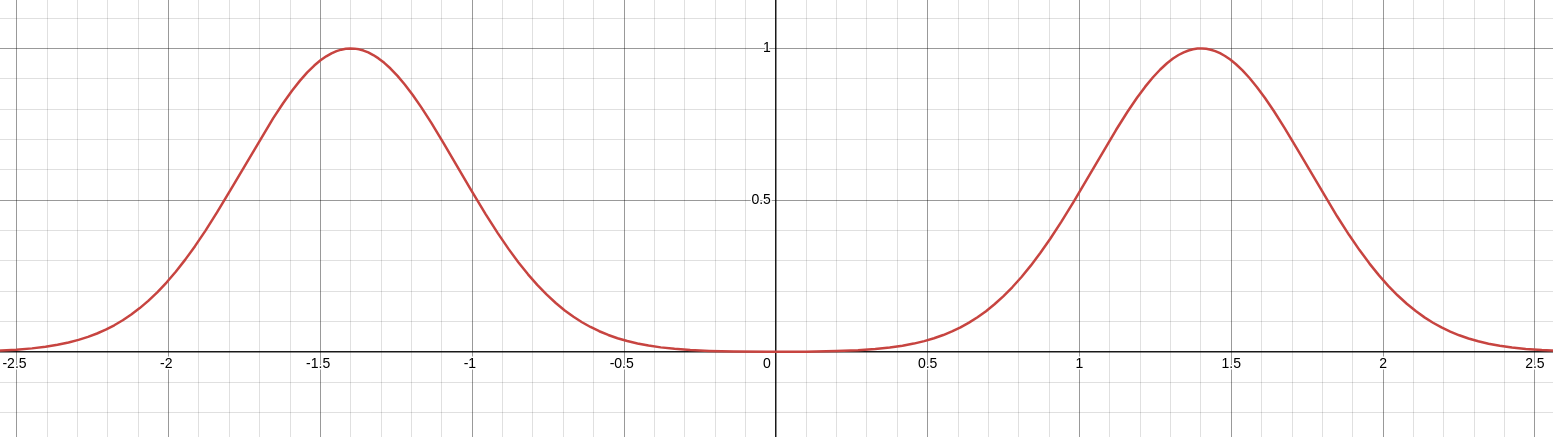
\includegraphics[width=0.9\textwidth]{fig/part-1/densi_spec_sym}
	\caption{Exemple de densité spectrale d'un signal réel \textbf{ESP A 1,4}}
	\label{fig:densi_spec_sym}
\end{figure}
\\
Même problème avec la covariance : sachant l'égalité des deux notions de fréquences moyenne (\cref{eq:esp_freq}, \cref{prop:mom_freq}), on peut définir la covariance temps-fréquence d'un signal $x$ par :
\begin{align*}
	\text{Cov}(x) \defeq \text{Cov}\big(t,\phi'(t) \big) 
	&= \esp[\densit]{t\phi'(t)} - \esp[\densit]{t} \esp[\densit]{\phi'(t)} \\
	&= \esp[\densit]{t\phi'(t)} - \esp[\densit]{t} \esp[\densis]{\nu}	
\end{align*}
\\
Ce coefficient est sensé mesurer une corrélation entre l'évolution d'un signal au cours du temps avec ses fréquences. S'il est réel, alors  $\text{Cov}(x)$ sera toujours nulle ; de là à en conclure que la fréquence instantanée de n'importe quel signal (réel) est toujours décorrélée du temps serait, pour le moins, insatisfaisant.
\\

Pour résoudre le problème, une méthode consiste à construire un nouveau signal $\SA{x}$ en supprimant les fréquences négatives de $x$ :
\[\mathcal{F}\big[\SA{x}\big] = 2\one_{\R^+}\fou{x}\]
où $\one_E$ est la fonction indicatrice sur l'ensemble $E$ et où le facteur 2 assure la conservation de l'énergie du signal. Cela mène à la définition :

\begin{definition}[Transformée de Hilbert et en SA]\label{def:transfo_sa&hilbert}
	On appelle \emph{transformé de Hilbert de} $x$, l'application :
	\begin{equation}\label{eq:transfo_Hilb}
		\mathcal{H}[x] :\ \begin{aligned} 
			\R \quad &\lr\qquad\quad \C \\	
			t\quad &\longmapsto\ \frac{1}{\pi}\fint_\R \frac{x(s)}{t-s}ds %=  \frac{1}{\pi}\left(\vpC\right)*x
		\end{aligned}
	\end{equation}
	où l'intégrale barré représente la \emph{valeur principale de Cauchy} (voir \cref{ann:transfo_SA} pour plus de détail) :
	\begin{align*}
		\fint_\R \frac{x(s)}{t-s}ds &\defeq \lim_{\varepsilon\lr0^+} \int_{-\infty}^{-\varepsilon} \frac{\varphi(t)}{t}dt + \int_{+\varepsilon}^{+\infty} \frac{\varphi(t)}{t}dt 
		%\\ &= \int_0^{+\infty} \frac{\varphi(t) - \varphi(-t)}{t}dt
	\end{align*}
	Avec, on définit la \emph{transformée en signal analytique} (SA) de tout signal $x$ comme l'unique application $\SA{x}$ telle que $\ \Fou{\SA{x}\big.}= 2\one_{\R^+}\fou{x}$. Elle est donnée par la formule :
	\begin{equation}\label{eq:transfo_SA}
		\SA{x} :\ \begin{aligned} 
			\R \quad &\lr\qquad\quad \C \\	
			t\quad &\longmapsto\ x(t) + i\mathcal{H}[x](t) %= x(t) + \frac{i}{\pi}\fint_\R \frac{x(s)}{t-s}ds
		\end{aligned}
	\end{equation}
	Plus généralement, tout signal dont le spectre est à support dans $\R^+$ sera dit \emph{analytique}.
\end{definition}
\skipl

Pour mieux comprendre ce que fait la transformation en signal analytique, revenons sur la notion de fréquence instantanée pour les signaux réels.
%Par souci de commodité, plutôt que redéfinir tout le vocabulaire développé plus haut (fréquence moyenne, temps moyen, \etc) pour les signaux réel via la transformation $\mathcal{A}$, dans la suite du mémoire on travaillera directement avec $\SA{x}$. %^(et on verra que c'est essentiel).
\\



\subsubsection{\wip Interprétabilité de la transformée en SA ou le lien avec le théorème de Bedrosian}\label{ann:bedrosian}

Pour définir l'amplitude et la phase instantanée d'un signaux réel, on par a nouveau du cas le plus simple. Si $x$ est un signal pur, il va s'écrire :
\[x(t) = a \cos(2\pi\nu t + \varphi),\qquad a,\nu,\varphi\in\R\]
\\
Pour généraliser cette écriture, il suffit donc de poser les amplitude et phase instantanée $a$ et $\phi$ telles que :
\[x(t) = a(t) \cos\big( \phi(t) \big)\]
\\
Contrairement au cas complexe, ici la pair $(a,\phi)$ n'est pas unique et pour contraindre ce choix, on s'appuie sur la transformée $\SA{x}$. Sachant que, dans le cas $x(t)\in\R$, la transformée de Hilbert est à valeur dans $\R$ (intégrale d'une fonction réelle), on a :
\[\SA{x}(t) = a(t)e^{i\phi(t)}\quad \Lr\quad \left\{\begin{aligned}x(t) &= \Re e \SA{x} = a(t) \cos\phi(t) \\ \mathcal{H}[x](t) &= \Im m \SA{x} = a(t) \sin\phi(t)
\end{aligned}\right.\]
\\
D'où la définition :
\begin{definition}[Amplitude et phase instantanée]\label{def:ampli-phase_instant}
	L'\emph{amplitude instantanée} $a_x$ et la \emph{phase instantanée} $\phi_x$ de tout signal $x$ réel sont définies comme étant respectivement l'amplitude et la phase de $\SA{x}$ :
	\begin{align}\label{eq:ampli-phase_instant}
		a_x &= \big|\SA{x}\big|   &   \phi_x &= \arg\big(\SA{x}\big)
	\end{align}
	De même, les \emph{impulsion} et \emph{fréquence instantanée} sont données par $\ \phi'_x\ $ et $\ \nicefrac{1}{2\pi}\phi_x'$.
\end{definition}
\skipl

Si un signal est présenté sous la forme  $\ x=a\cos\phi$, rien n'implique que $a$ et $\phi$ correspondent bel et bien à l'amplitude et la phase instantanée. Si ce n'est pas le cas, c'est que cette décomposition n'est ``pas la bonne'', en cela qu'elles ne s’interprètent pas comme l'on aimerait.
\\
Aussi, quand bien même $x$ peut toujours être écrit comme partie réel de sa transformé en SA, cette écriture n'est nécessairement toujours satisfaisante. Pour le comprendre, détaillons le cas où $x$ s'écrit comme produit de deux signaux pures (\cref{fig:exemple_tSA_1/2}) :
\[x_1(t) = \cos (2\pi\nu_1t)\cos (2\pi\nu_2t)\]

\begin{figure}[h]\centering
	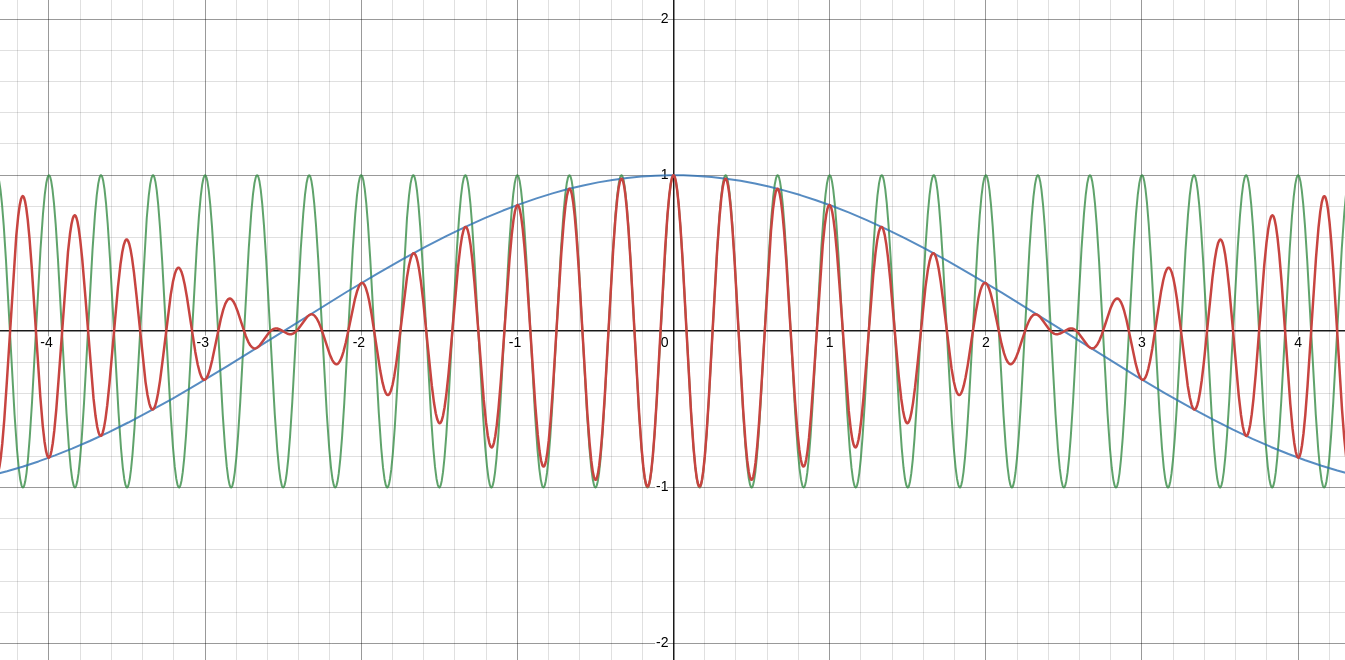
\includegraphics[width=0.48\textwidth]{fig/part-1/ex SA - 11.png}
	\hfill
	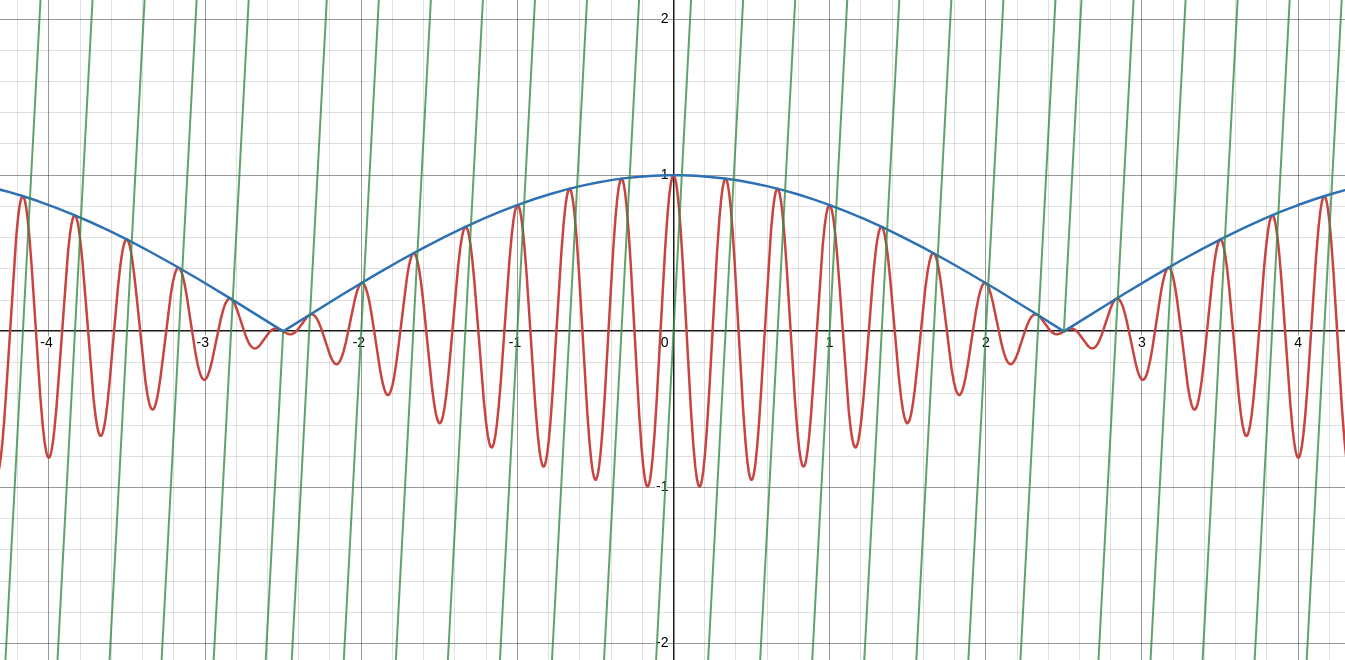
\includegraphics[width=0.48\textwidth]{fig/part-1/ex SA - 12.png}
	\caption{Représentation graphique du signal $x$ (rouge) avec $\nu_1=3$ et $\nu_2=0.1$. Sur l'image de gauche, avec signaux de fréquences pures (bleu et vert). Sur l'image de droite, avec son amplitude (bleu) et sa phase instantanée (vert). Les discontinuités de la phase sont dû à l'arrondi à $2\pi$  près de l'argument de $\SA{x_1}$ et à la façon dont il est calculé lorsque le signal s'annule (mise à 0). Voir \href{https://www.desmos.com/calculator/gcedcdfkhr}{ici} pour un graphique dynamique.}
	\label{fig:exemple_tSA_1/2}
\end{figure}

\noindent
On montre sans mal\footnote{\itshape
	$\fou{x}_1$ est donné par 4 Diracs, en ne gardant que ce non nul sur $\R^+$ on obtient le spectre de $\SA{x_1}$ et il reste plus qu'à inverser la transformée de Fourier.}
que si $\ \nu_1\geq\nu_2$, alors la transformée en SA de $x_1$ s'écrit :
\[\SA{x_1} = \cos \left(2\pi\nu_2 t\right) e^{2i \pi\nu_1 t}\]
\\
Le signal $\SA{x_1}$ n'est ici pas sous forme exponentielle à proprement parler puisque le cosinus peut être négatif (pour s'y ramener, il suffit de passer le cos en valeur absolue et d'ajouter $\pi$ à l'argument lorsque nécessaire) mais l’avantage de cette forme est qu'elle fait clairement apparaître les fréquences $\nu_{1,2}$. En particulier, la fréquence instantanée du signal est la plus grandes des deux fréquences $\nu_1$ et $\nu_2$. La plus petite, elle, se retrouve dans l'amplitude. 
\\
Ce résultat est rassurant en cela qu'il est plus naturel de voir le cosinus de basse fréquence comme modulant celui de haute fréquence que l'inverse comme on le voit sur la première image de la figure \ref{fig:exemple_tSA_1/2}. 
\\
Aussi, en mettant les hautes fréquences du signal dans la fréquence instantanée, on s'assure de limiter les variations de l'amplitude. Cela apporte bien plus de contrainte en terme de décomposition $(a_{x_1},\phi_{x_1})$, en cela qui si l'inverse étant vrai, alors toute les fréquences pourrait être envoyé dans l'amplitude, ce qui laisserait la phase invariante.
\\

Cela étant dit, lorsque l'on fait varier $\nu_1$ et $\nu_2$, le résultat n'est pas toujours si intuitif. C'est notamment le cas lorsque les deux deviennent de plus en plus proche :

\begin{figure}[h]\centering
	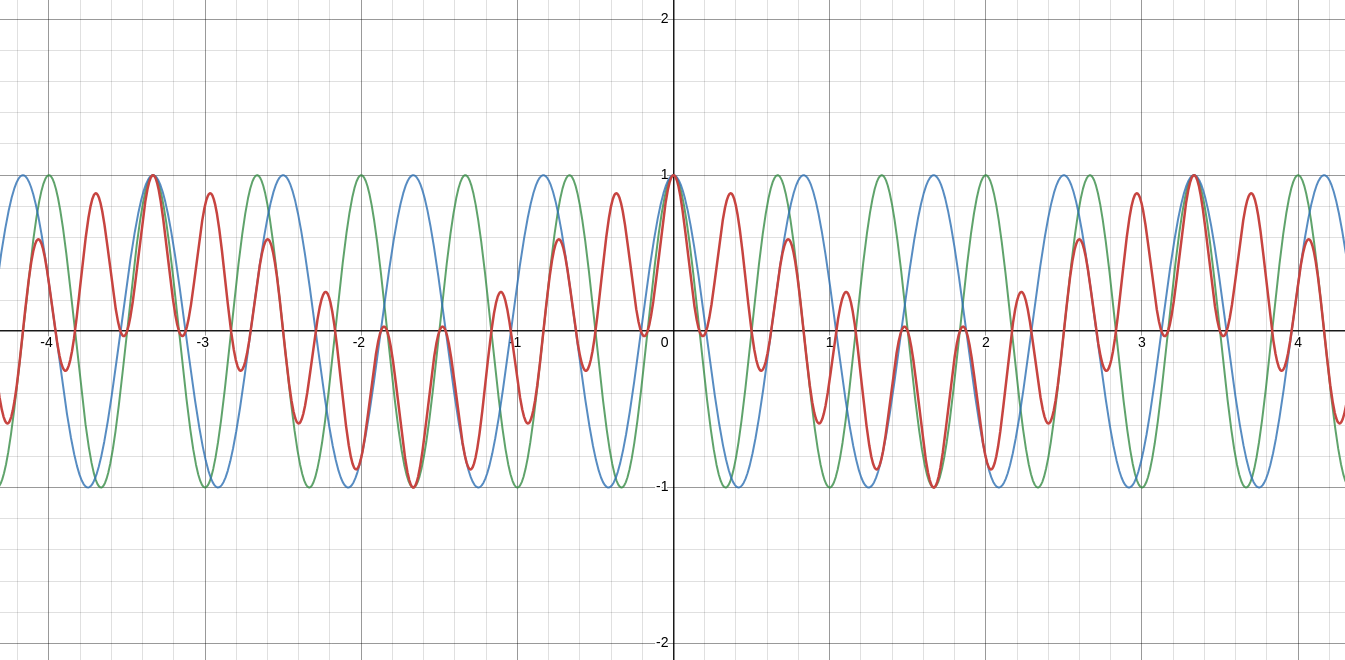
\includegraphics[width=0.48\textwidth]{fig/part-1/ex SA - 21.png}\hfill
	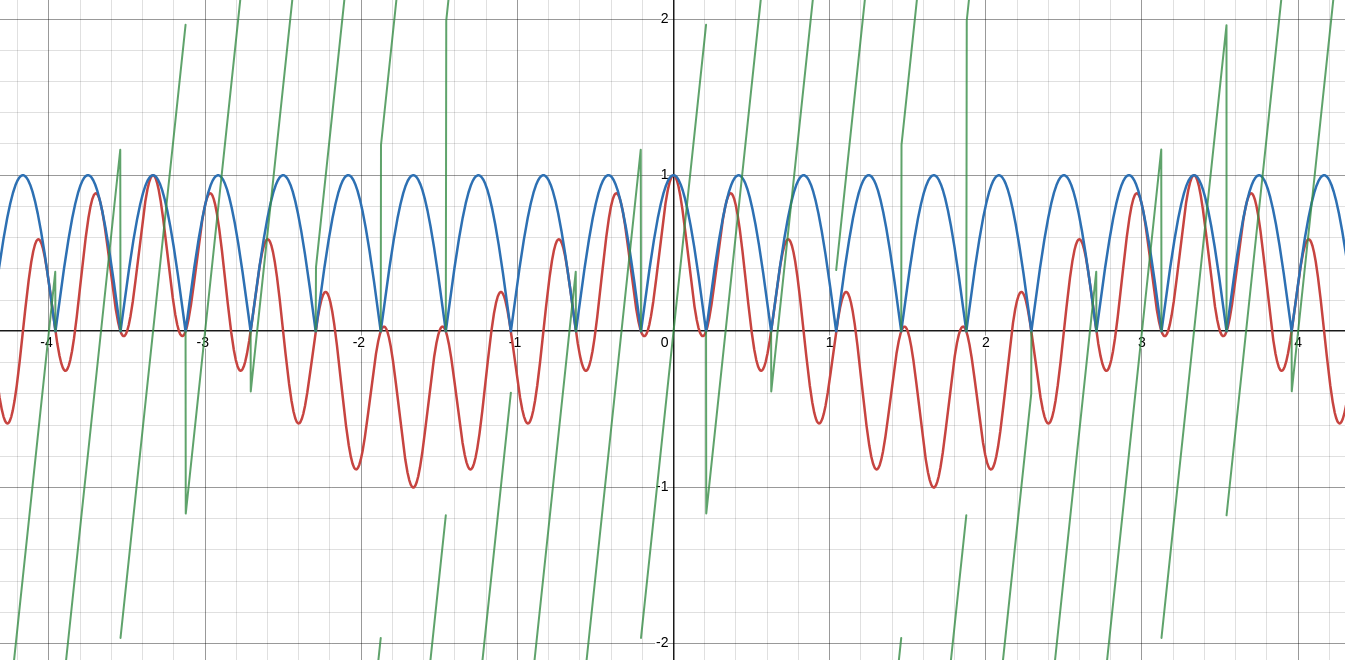
\includegraphics[width=0.48\textwidth]{fig/part-1/ex SA - 22.png}
	\caption{Idem que pour la figure \ref{fig:exemple_tSA_1/2} précédente, avec cette fois $\nu_1=1.5$ et $\nu_2=1.3$.}
	\label{fig:exemple_tSA_2/2}
\end{figure}

Pour comprendre pourquoi l'amplitude ne fait pas ce qu'on attendrait d'elle, est introduit le théorème de Bedrosian :

\begin{theoreme}[de Bedrosian]\label{theo:2Bedrosian}
	Dans sa formulation la plus générale, le théorème de Bedrosian énonce que si deux fonctions $f,g\in L^2(\R)$ sont telles l'une des trois assertions suivantes est vraie :
	\begin{itemize}%[label=\textit{\arabic*}. ]
		\item 
		\item $\exists \lambda\in\R^+\ |\ \supp \fou{f} \subset [-\lambda, +\infty[,\ \supp \fou{g} \subset [\lambda, +\infty[$\label{item:1condi_theo2Bedrosian}
		
		\item $\exists \lambda\in\R^+\ |\ \supp \fou{f} \subset ]-\infty, \lambda],\ \supp \fou{g} \subset ]-\infty,-\lambda]$ \label{item:2condi_theo2Bedrosian}
		
		\item $\exists (\lambda_1,\lambda_2)\in \R^+\times\R^+ \setminus\{(0,0)\}\ |\ \supp \fou{f} \subset [-\lambda_1, \lambda_2],\ \supp \fou{g} \subset \R\setminus[-\lambda_2,\lambda_1]$
		
	\end{itemize}
	alors la transformée de Hilbert de leur produit s'écrit (voir \cite{wang_simple_2009} pour une démonstration) :
	\begin{equation}\label{eq:2Bedrosian}
		\hilb{fg} = f\hilb{g}
	\end{equation}
\end{theoreme}

Dans le cas d'un signal réel, suivant la \cref{def:ampli-phase_instant} on peut écrire $\ x=a_x\cos \phi_x$.
Comme $a_x$ et $\cos \phi_x$ sont réelles, seule la troisième condition du théorème de Bedrosian peut être satisfaite pour peu que $\lambda_1=\lambda_2$. Ainsi :

\begin{corollaire}\label{coro:AM-FM}
	Toujours avec les même notations, si $a_x\in L^2(\R)$, $\cos\phi_x\in L^2(\R)$ et qu'il existe $\lambda\in\R^{+_*}$ tel que :
	\begin{equation}\label{eq:condiBedro_AM-FM}
		\supp \Fou{a_x} \subset [-\lambda, \lambda],\quad \supp \Fou{\cos\phi_x} \subset \R\setminus[-\lambda,\lambda]
	\end{equation}
	Alors on a :
	\begin{align}\label{eq:result_AM-FM}
		\hilb{x} &= a_x\hilb{\cos \phi_x}  &  \qquad\qquad&\text{et si }a_x(t)\neq 0,  &  \hilb{\cos \phi_x}(t) = \sin\phi_x(t)
	\end{align}
\end{corollaire}
\skipl

Pour interpréter ce \namecref{coro:AM-FM}, prenons un autre exemple : $\ x_2(t) = a(t)\cos(2\pi \nu_0 t)$. Sa transformé de Fourier est donnée par :
\begin{align*}
	\fou{x}_2(\nu) &= \fou{a}(\nu)*\frac{1}{2}\Big(\delta(\nu-\nu_0) + \delta(\nu+\nu_0)\Big) \\
	&= \frac{1}{2}\Big(\fou{a}(\nu+\nu_0) + \fou{a}(\nu-\nu_0)\Big)
\end{align*}
\\
Graphiquement, la transformé de Fourier de $x_2$ duplique le graphe de $\fou{a}$ en $\pm\nu_0$ et somme les deux. La condition \eqref{eq:condiBedro_AM-FM} du \cref{coro:AM-FM} demande alors que $\nu_0$ soit choisie de telle sorte que :
\[\supp \Fou{a}\subset[-\nu_0, \nu_0]\]
\\
C'est-à-dire qu'il n'y ait pas de chevauchement entre les deux courbes $\ \Gamma_\pm : \nu \longmapsto \fou{a}(\nu\mp\nu_0) $ (voir \cref{fig:alising-ish} ci-dessous). Moralement, cela assure qu'en ne prenant que la partie positive du spectre de $x_2$, l'on ne ramène pas avec une partie de $\fou{a}(\nu+\nu_0)$. Quant bien même cette explication est simpliste puisqu'ici $\phi$ est linaire, on peut voir que le phénomène est finalement très proche de celui d'aliasing.
\\

\begin{figure}[h]\centering
	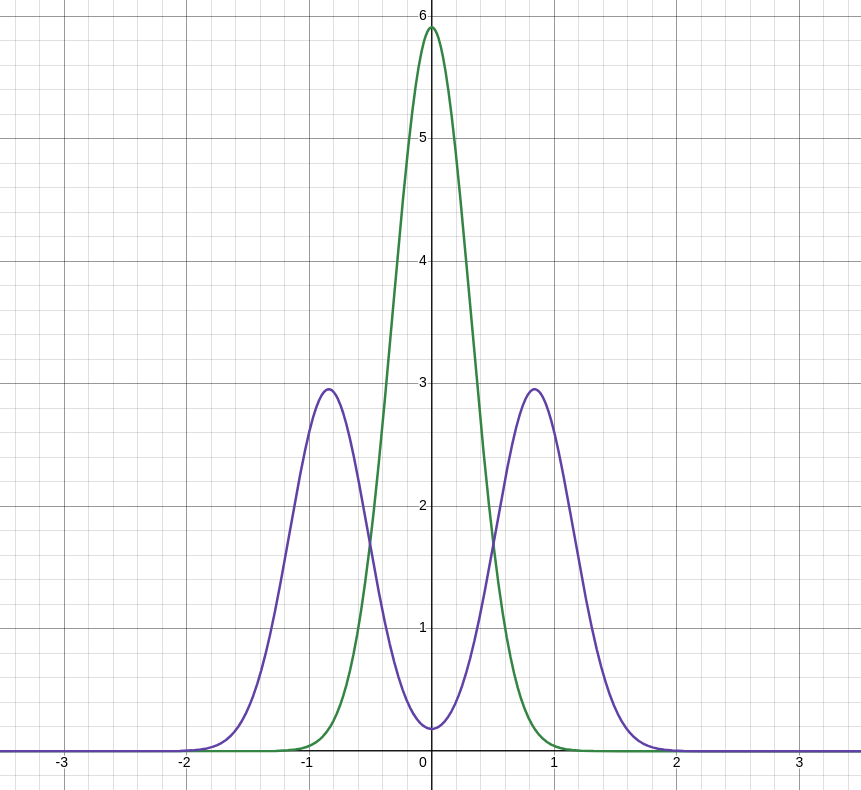
\includegraphics[width=0.45\textwidth]{fig/part-1/bedro condi 1.png} 
	\hfill
	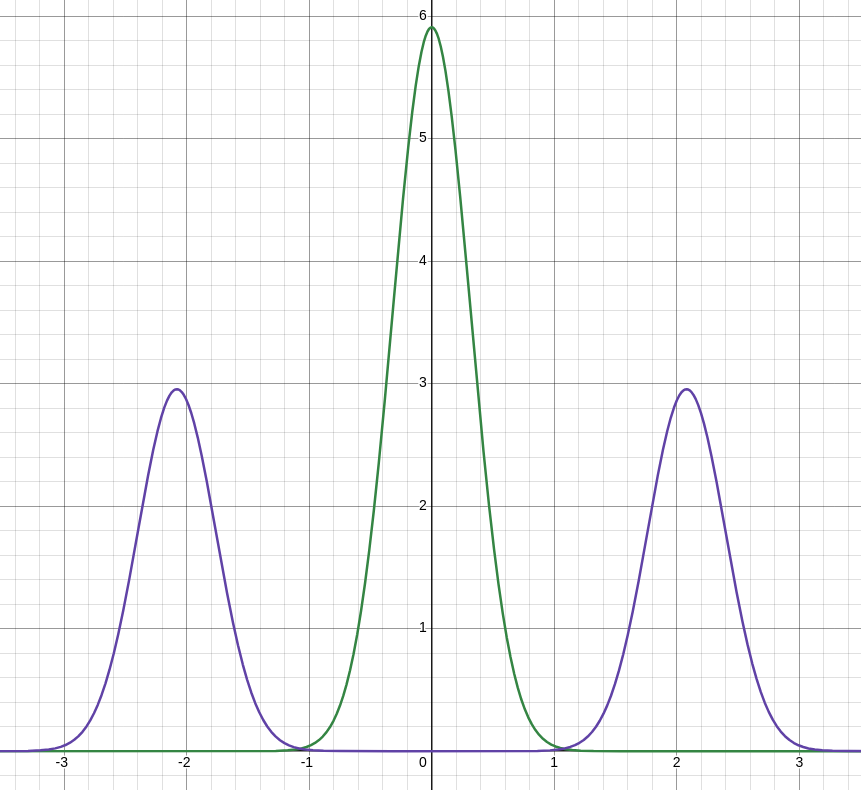
\includegraphics[width=0.45\textwidth]{fig/part-1/bedro condi 2.png} 
	\caption{Sur les deux graphiques sont représentés en vert $\fou{a}$ et en violet $\fou{x}_2$. Dans le premier cas l'hypothèse de Bedrosian et respectée mais pas dans le second.}
	\label{fig:alising-ish}
\end{figure}


Pour revenir sur l'exemple $x_1$ précédent, dans la seconde figure \ref{fig:exemple_tSA_2/2}, l'amplitude ne colle plus à l'interprétation que l'on voudrait justement parce que la condition de Bedrosian n'est plus respecter (à savoir $\nu_1\geq 2\nu_2$). 




\subsection{Calcul des phases}\label{ann:demo_phases_2var}

\begin{demo}[de la formule \eqref{eq:phaset_2var}, \cref{prop:phases_2var}]
	Pour la phase totale, on note cette fois $\mathcal{V} = \begin{pmatrix} \cos\chi \\ -i\sin\chi \end{pmatrix}$ et on a :
	\begin{align*}
		\big\langle \x(t), \x(t_0)\big\rangle &= \Big\langle a(t)e^{i\varphi(t)}R_{\theta(t)}\mathcal{V}(t), a(t_0)e^{i\varphi(t_0)}R_{\theta(t_0)}\mathcal{V}(t_0) \Big\rangle \\
		&= a(t)e^{i\varphi(t)} a(t_0)e^{-i\varphi(t_0)} \Big\langle R_{\theta(t)}\mathcal{V}(t), R_{\theta(t_0)}\mathcal{V}(t_0) \Big\rangle \\
		%&= a(t_0)a(t)e^{i(\varphi(t_0)-\varphi(t))}\Big\langle \mathcal{V}(t_0), R_{\theta(t_0)}^{-1}R_{\theta(t)}\mathcal{V}(t) \Big\rangle \\
		&= a(t_0)a(t)e^{i(\varphi(t)-\varphi(t_0))}\Big\langle R_{\theta(t)- \theta(t_0)}\mathcal{V}(t), \mathcal{V}(t_0) \Big\rangle
	\end{align*}
	Pour alléger les notations, on note $\ \Delta y =y(t)-y(t_0)$, $\ y_1=y(t_0)\ $ et $\ y_2=(t)\ $ pour $\ y=\varphi,\theta,\chi$. Le produit hermitien à droite s'écrit alors :
	\begin{align*}
		\Big\langle R_{\Delta\theta}\mathcal{V}(t), \mathcal{V}(t_0) \Big\rangle &=   \Big(\cos\Delta\theta \cos\chi_2 + i\sin\Delta\theta \sin\chi_2 \qquad \sin\Delta\theta \cos\chi_2 - i\cos\Delta\theta \sin\chi_2\Big) \begin{pmatrix} \cos\chi_1 \\ i\sin\chi_1 \end{pmatrix} \\
		&= \cos\chi_1\Big(\cos\Delta\theta \cos\chi_2 + i\sin\Delta\theta \sin\chi_2\Big) + i\sin\chi_1\Big(\sin\Delta\theta \cos\chi_2 - i\cos\Delta\theta \sin\chi_2\Big) \\
		&= \cos\Delta\theta \Big(\cos\chi_1 \cos\chi_2 + \sin\chi_1 \sin\chi_2\Big) + i\sin\Delta\theta \Big( \cos\chi_1 \sin\chi_2 + \sin\chi_1\cos\chi_2\Big) \\
		&= \cos\Delta\theta \cos\Delta\chi + i\sin\Delta\theta \sin(\chi_1+\chi_2)
	\end{align*}
	\\
	D'où la phase totale :
	\begin{align*}
		\phaset(\x) = \arg\big\langle \x(t), \x(t_0)\big\rangle &= \arg\left( a(t_0)a(t)e^{i(\varphi(t) - \varphi(t_0))}\Big( \cos\Delta\theta \cos\Delta\chi + i\sin\Delta\theta \sin(\chi_1+\chi_2) \Big) \right) \\
		&= \varphi(t) - \varphi(t_0) + \arg\Big( \cos\Delta\theta \cos\Delta\chi + i\sin\Delta\theta \sin(\chi_1+\chi_2) \Big)
	\end{align*}
	et l'argument restant s'écrit comme une arctangente, donnant :
	\begin{align*}
		\phaset(\x) &= \varphi(t)-\varphi(t_0) + \arctan\frac{\sin\Delta\theta \sin(\chi_1+\chi_2)}{\cos\Delta\theta \cos\Delta\chi} \\
		&= \varphi(t)-\varphi(t_0) + \arctan \left( \tan\Delta\theta\frac{\sin(\chi_1+\chi_2)}{\cos\Delta\chi} \right) \\
		&= \cdots
	\end{align*}
\end{demo}

\begin{demo}[de la formule \eqref{eq:phased_2var}, \cref{prop:phases_2var}]
	Par souci de lisibilité, on note $\ \mathcal{U} = R_{\theta} \begin{pmatrix} \cos\chi \\ -i\sin\chi \end{pmatrix} = \begin{pmatrix} \cos\theta(t) \cos\chi(t) + i\sin\theta(t) \sin\chi(t) \\ \sin\theta(t) \cos\chi(t) - i\cos\theta(t) \sin\chi(t) \end{pmatrix}$, de sorte que la dérivée de $\ \x=ae^{i\varphi}\mathcal{U}\ $ s'écrive :
	\[\dot{\x} = a'e^{i\varphi}\mathcal{U} + ia\varphi'e^{i\varphi} \mathcal{U} + ae^{i\varphi}\theta'\begin{pmatrix} -\sin\theta \cos\chi + i\cos\theta \sin\chi \\ \cos\theta \cos\chi + i\sin\theta \sin\chi \end{pmatrix} + ae^{i\varphi}\chi'\begin{pmatrix} -\cos\theta \sin\chi + i\sin\theta \cos\chi \\ -\sin\theta \sin\chi - i\cos\theta \cos\chi \end{pmatrix}\]
	\\
	Les vecteurs des deux derniers membres s'expriment en fonction des composantes $\ \mathcal{U}_{1,2}\ $ de $\ \mathcal{U}$ :
	\begin{align*}
		\begin{pmatrix} -\sin\theta \cos\chi + i\cos\theta \sin\chi \\ \cos\theta \cos\chi + i\sin\theta \sin\chi \end{pmatrix} &= \begin{pmatrix} -\mathcal{U}_2 \\ \mathcal{U}_1 \end{pmatrix}  &
		\begin{pmatrix} -\cos\theta \sin\chi + i\sin\theta \cos\chi \\ -\sin\theta \sin\chi - i\cos\theta \cos\chi \end{pmatrix} &= i\begin{pmatrix} \congu{\mathcal{U}}_2 \\ -\congu{\mathcal{U}}_1 \end{pmatrix}
	\end{align*}
	\\
	Le produit hermitien $\langle \dot{\x}, \x \rangle$ s'écrit alors :
	\begin{align*}
		\langle \dot{\x}, \x \rangle 
		&= \left\langle a'e^{i\varphi}\mathcal{U} + ia\varphi'e^{i\varphi} \mathcal{U} + ae^{i\varphi}\theta'\begin{pmatrix} -\mathcal{U}_2 \\ \mathcal{U}_1 \end{pmatrix} + iae^{i\varphi}\chi'\begin{pmatrix} \congu{\mathcal{U}}_2 \\ -\congu{\mathcal{U}}_1 \end{pmatrix}, ae^{i\varphi}\mathcal{U} \right\rangle \\
		&= \left\langle a'\mathcal{U} + ia\varphi' \mathcal{U} + a\theta'\begin{pmatrix} -\mathcal{U}_2 \\ \mathcal{U}_1 \end{pmatrix} + ia\chi'\begin{pmatrix} \congu{\mathcal{U}}_2 \\ -\congu{\mathcal{U}}_1 \end{pmatrix}, a\mathcal{U} \right\rangle \\
		&= aa' \big\langle \mathcal{U}, \mathcal{U}\big\rangle  + ia^2\varphi' \big\langle \mathcal{U}, \mathcal{U}\big\rangle  + a^2\theta'\left\langle \begin{pmatrix} -\mathcal{U}_2 \\ \mathcal{U}_1 \end{pmatrix}, \mathcal{U} \right\rangle + ia^2\chi'\left\langle \begin{pmatrix} \congu{\mathcal{U}}_2 \\ -\congu{\mathcal{U}}_1 \end{pmatrix}, \mathcal{U} \right\rangle
	\end{align*}
	où les deux derniers produits hermitiens donnent :
	\begin{align*}
		\left\langle \begin{pmatrix} -\mathcal{U}_2 \\ \mathcal{U}_1 \end{pmatrix}, \mathcal{U} \right\rangle &= -\mathcal{U}_2\congu{\mathcal{U}}_1 + \mathcal{U}_1\congu{\mathcal{U}}_2 \\
		&= 2i\Im m\big(\mathcal{U}_1 \congu{\mathcal{U}}_2\big) \\
		&= 2i\Im m\Big(\big( \cos\theta \cos\chi + i \sin\theta \sin\chi \big) \big( \sin\theta \cos\chi + i \cos\theta \sin\chi \big)\Big) \\
		&= 2i\big(\cos^2\theta \cos\chi \sin\chi + \sin^2\theta \sin\chi \cos\chi \big) \\
		&= 2i \cos\chi \sin\chi \\
		&= i\sin2\chi 
		\\ \\
		\left\langle \begin{pmatrix} \congu{\mathcal{U}}_2 \\ -\congu{\mathcal{U}}_1 \end{pmatrix}, \mathcal{U} \right\rangle &= \congu{\mathcal{U}_2\mathcal{U}_1} - \congu{\mathcal{U}_1\mathcal{U}_2} = 0
	\end{align*}
	\\
	D'où, sachant que $\ \|\x\|^2=a^2\ $ et $\ \|\mathcal{U}\|=1$, la formule :
	\begin{align*}
		\frac{\Im m\big\langle \dot{\x}, \x\big\rangle}{\|\x\|^2} &= \frac{1}{a^2}\Im m\Big(aa' \big\langle \mathcal{U}, \mathcal{U}\big\rangle  + ia^2\varphi' \big\langle \mathcal{U}, \mathcal{U}\big\rangle + ia^2\theta' \sin2\chi \Big) \\
		&= \frac{1}{a^2} \Big( a^2\varphi' \|\mathcal{U}\|^2 + a^2\theta' \sin2\chi \Big) \\
		&= \varphi' + \theta' \sin2\chi
	\end{align*}
\end{demo}
\skipl


\subsection{\todo Lien entre Poincaré et Bloch (EN VRAC)}

\subsubsection{\todo Lien entre les deux types de signaux}

Soit le signal :
\[\x_B(\varphi, \theta, \chi) = e^{i\varphi} \begin{pmatrix}
	\cos \chi/2 \\ e^{i\theta}\sin\chi/2\end{pmatrix}\]
Pour le réécrire en terme de vecteur AM-FM-PM, il faut faire apparaître une matrice de rotation, matrice qui est diagonalisable dans $\C^{n\times n}$ via la relation :
\begin{align*}
	&\begin{pmatrix} 
		\cos \alpha & -\sin \alpha \\ 
		\sin\alpha & \cos\alpha 
	\end{pmatrix} = \frac{1}{2} \begin{pmatrix} 
		1 & -1 \\ i & i
	\end{pmatrix}\begin{pmatrix} 
		e^{-i\alpha} & 0 \\ 
		0 & e^{i\alpha} 
	\end{pmatrix}\begin{pmatrix} 
		1 & -i \\ -1 & -i
	\end{pmatrix}\\
	&\Llr\quad \begin{pmatrix} 
		1 & -i \\ -1 & -i
	\end{pmatrix}\begin{pmatrix} 
		\cos \alpha & -\sin \alpha \\ 
		\sin\alpha & \cos\alpha 
	\end{pmatrix} \begin{pmatrix} 
		1 & -1 \\ i & i
	\end{pmatrix} = 2 \begin{pmatrix} 
		e^{-i\alpha} & 0 \\ 
		0 & e^{i\alpha} 
	\end{pmatrix}
\end{align*}
\\
Cela permet d'écrire :
\begin{align*}
	\x_B(\varphi, \theta, \chi) &= e^{i\varphi} e^{i\theta/2}\begin{pmatrix}
		e^{-i\theta/2} & 0 \\
		0 & e^{i\theta/2}
	\end{pmatrix}\begin{pmatrix} 
		\cos \chi/2 \\ 
		\sin \chi/2 
	\end{pmatrix} \\
	&= \frac{1}{2}e^{i\varphi} e^{i\theta/2}\begin{pmatrix} 
		1 & -i \\
		-1 & -i
	\end{pmatrix}\begin{pmatrix} 
		\cos \theta/2 & -\sin \theta/2 \\ 
		\sin \theta/2 & \cos \theta/2 
	\end{pmatrix} \begin{pmatrix} 
		1 & -1 \\ i & i
	\end{pmatrix}\begin{pmatrix} 
		\cos \chi/2 \\ 
		\sin\chi/2
	\end{pmatrix} \\
	&= \frac{\sqrt{2}}{2}e^{i(\varphi + \theta/2)}U R_{\theta/2} \begin{pmatrix} 
		\cos \chi/2 - \sin\chi/2 \\ 
		i\big(\cos\chi/2 + \sin\chi/2\big)
	\end{pmatrix}   & &\text{où }\quad U = \frac{\sqrt{2}}{2}\begin{pmatrix} 
		1 & -i \\ -1 & -i
	\end{pmatrix}\in \U{2} \\
\end{align*}
\\
Ensuite, pour réduire les sommes dans le vecteur de droite, on a rappel les formules :
\begin{align*}
	\cos\left( \frac{\pi}{2} \pm \alpha\right) &= \frac{\sqrt{2}}{2}\big( \cos\alpha \mp \sin \alpha \big) & \sin\left( \frac{\pi}{2} \pm \alpha\right) &= \frac{\sqrt{2}}{2}\big( \cos\alpha \pm \sin \alpha \big)
\end{align*}
\\ 
On a donc deux choix pour chaque composante du vecteur mais celle avec un signe moins son préférable sachant que : 
\begin{align*}
	\cos\left( \frac{\pi}{2} - \alpha\right) &= \sin(\alpha) &  \sin\left( \frac{\pi}{2} - \alpha\right) &= \cos(\alpha)
\end{align*}
\\
On choisi donc la seconde formule pour la première composante et la premier pour la seconde composante, donnant :
\begin{align*}
	\x_B(\varphi, \theta, \chi) &= \frac{\sqrt{2}}{2}e^{i(\varphi + \theta/2)}U R_{\theta/2} \begin{pmatrix} 
		\cos \chi/2 - \sin\chi/2 \\ 
		i\big(\cos\chi/2 + \sin\chi/2\big)
	\end{pmatrix} \\
	&= e^{i(\varphi + \theta/2)}U R_{\theta/2} \begin{pmatrix} 
		\sin\left( \frac{\pi}{2} - \chi/2\right) \\ 
		i\cos\left( \frac{\pi}{2} - \chi/2\right)
	\end{pmatrix} \\
	&= e^{i(\varphi + \theta/2)}U R_{\theta/2} \begin{pmatrix} 
		\cos \chi/2 \\ 
		i\sin \chi/2
	\end{pmatrix}
\end{align*}
\\
Ne reste alors plus qu'à ajuster les signes pour obtenir une écriture de signal $\x_P$ AM-FM-PM :
\begin{align*}
	\x_B(\varphi, \theta, \chi) &= e^{i(\varphi + \theta/2)}U R_{\theta/2} \begin{pmatrix} 
		\cos \chi/2 \\ 
		i\sin \chi/2
	\end{pmatrix} \\
	&= U e^{i(\varphi + \theta/2)} R_{\theta/2} \begin{pmatrix} 
		\cos (-\chi/2) \\ 
		-i\sin (-\chi/2)
	\end{pmatrix}
\end{align*}
En somme :
\begin{align} \label{eq:bloch2poinca}
	\x_B(\psi, \alpha, \beta) &= U \x_P(\psi + \alpha/2, \alpha/2, -\beta/2)  & 
	\x_P(\varphi, \theta, \chi) = U^\dagger 	\x_B(\varphi-\theta, 2\theta, -2\chi)	
\end{align}
\skipl 



\subsubsection{\todo Lien entre les projections}

Avec la formule \eqref{eq:bloch2poinca} ci-dessus, on a :

\begin{align}
	\rho_B(\alpha, \beta) &= U \rho_P(\alpha/2, -\beta/2)U^\dagger  & 
	\rho_P(\theta, \chi) &= U^\dagger \rho_B(2\theta, -2\chi) U
	%\\ \Llr\ \rho_B(\alpha, \beta) U &= U \rho_P(\alpha/2, -\beta/2) & \Llr\ \rho_P(\theta, \chi) U^\dagger &= U^\dagger \rho_B(2\theta, -2\chi) 
\end{align}
\\
Mais on a aussi, dans la base Pauli :
\begin{align*}
	\sigma_1 &= \begin{pmatrix} 0 & 1 \\ 1 &  0 \end{pmatrix}  &
	\sigma_2 &= \begin{pmatrix} 0 & -i \\  i &  0 \end{pmatrix}  &
	\sigma_3 &= \begin{pmatrix} 1 & 0 \\ 0 & -1 \end{pmatrix}
\end{align*}
les expressions :
\begin{align*}
	\rho_{P}(\theta, \chi) &= \frac{1}{2} \Big( id + \sin(2\theta) \cos(2\chi) \sigma_1 - \sin (2\chi) \sigma_2 + \cos(2\theta) \cos(2\chi) \sigma_3 \Big) \\ 
	\rho_{B}(\alpha, \beta) &= \frac{1}{2} \Big( id + \cos(\alpha) \sin(\beta) \sigma_1 + \sin(\alpha) \sin(\beta) \sigma_2 + \cos (\beta) \sigma_3 \Big)
\end{align*}
\skipl

Pour les lier, on pose $\ 2\theta = \nicefrac{\pi}{2} - \alpha\ $ et $\ 2\chi = \nicefrac{\pi}{2} - \beta$, donnant :
\begin{align*}
	\rho_P(\theta, \chi) - id 
	&= \sin(\nicefrac{\pi}{2} - \alpha) \cos(\nicefrac{\pi}{2} - \beta) \sigma_1 - \sin (\nicefrac{\pi}{2} - \beta) \sigma_2 + \cos(\nicefrac{\pi}{2} - \alpha) \cos(\nicefrac{\pi}{2} - \beta) \sigma_3 \\
	&= \cos(\alpha) \sin(\beta) \sigma_1 - \cos (\beta) \sigma_2 + \sin(\alpha) \sin(\beta) \sigma_3
\end{align*}
\\
Ce qui sous forme matricielle se réécrit :
\[\begin{pmatrix}
	\sin(2\theta) \cos(2\chi) \\ -\sin (2\chi) \\ \cos(2\theta) \cos(2\chi)
\end{pmatrix} = \begin{pmatrix}
	\cos(\alpha) \sin(\beta) \\ -\cos (\beta) \\ \sin(\alpha) \sin(\beta)
\end{pmatrix} = \begin{pmatrix}
	1 & 0 & 0 \\ 0 & 0 & -1 \\ 0 & 1 & 0
\end{pmatrix}\begin{pmatrix}
	\cos(\alpha) \sin(\beta) \\ \sin(\alpha) \sin(\beta) \\ \cos (\beta)
\end{pmatrix}\]
\\
Donc la passage de $\rho_B$ à $\rho_S$ se fait via un changement et d'angle et une rotation de $\nicefrac{\pi}{2}$ autour de $\sigma_1$.
\\

Même calcul, cette fois, en partant de \eqref{eq:bloch2poinca} :
\begin{align*}
	2\rho_P(\theta, \chi) &= 2U^\dagger \rho_B(2\theta, -2\chi) U \\
	&= U^\dagger \Big( id + \cos(2\theta) \sin(-2\chi) \sigma_1 + \sin(2\theta) \sin(-2\chi) \sigma_2 + \cos (-2\chi) \sigma_3 \Big) U \\
	&= id - \cos(2\theta) \sin(2\chi) U^\dagger \sigma_1 U - \sin(2\theta) \sin(2\chi) U^\dagger \sigma_2 U + \cos (2\chi) U^\dagger \sigma_3 U
\end{align*}
avec :
\begin{align*}
	U^\dagger \sigma_1 U &= \frac{1}{2} \begin{pmatrix} 
		1 & -1 \\ i & i
	\end{pmatrix} \begin{pmatrix} 
		0 & 1 \\ 1 &  0 
	\end{pmatrix} \begin{pmatrix} 
		1 & -i \\ -1 & -i
	\end{pmatrix} = \frac{1}{2} \begin{pmatrix} 
		-2 & 0 \\ 0 & 2
	\end{pmatrix} = -\sigma_3 \\
	U^\dagger \sigma_2 U &= \frac{1}{2} \begin{pmatrix} 
		1 & -1 \\ i & i
	\end{pmatrix} \begin{pmatrix} 
		0 & -i \\  i &  0 
	\end{pmatrix} \begin{pmatrix} 
		1 & -i \\ -1 & -i
	\end{pmatrix} = \frac{1}{2} \begin{pmatrix} 
		0 & -2 \\ -2 & 0
	\end{pmatrix} = -\sigma_1 \\
	U^\dagger \sigma_3 U &= \frac{1}{2} \begin{pmatrix} 
		1 & -1 \\ i & i
	\end{pmatrix}  \begin{pmatrix} 
		1 & 0 \\ 0 & -1 
	\end{pmatrix} \begin{pmatrix} 
		1 & -i \\ -1 & -i
	\end{pmatrix} = \frac{1}{2} \begin{pmatrix} 
		0 & -2i \\ 2i & 0
	\end{pmatrix} = \sigma_2
\end{align*}
\\
Qui donne :
\begin{align*}
	2\rho_P(\theta, \chi) &= id - \cos(2\theta) \sin(2\chi) U^\dagger \sigma_1 U - \sin(2\theta) \sin(2\chi) U^\dagger \sigma_2 U + \cos (2\chi) U^\dagger \sigma_3 U \\
	&= id + \cos(2\theta) \sin(-2\chi) \sigma_3 + \sin(2\theta) \sin(-2\chi)  \sigma_1 + \cos (-2\chi) \sigma_2 \\
	&= id + \sin(2\theta) \sin(2\chi)  \sigma_1 + \cos (2\chi) \sigma_2 + \cos(2\theta) \sin(2\chi) \sigma_3
\end{align*}
\\ 
Le tout reste cohérent et avec les notations :
\begin{align*}
	w_P(\theta, \chi) &= \begin{pmatrix}
		\sin(\theta) \cos(\chi) \\ -\sin (\chi) \\ \cos(\theta) \cos(\chi)
	\end{pmatrix}  &   w_B\big( \alpha, \beta \big) = \begin{pmatrix}
		\cos(\alpha) \sin(\beta) \\ \sin(\alpha) \sin(\beta) \\ \cos (\beta)
	\end{pmatrix}
\end{align*}
Cela devient :
\[w_P(2\theta, 2\chi) = \begin{pmatrix}
	1 & 0 & 0 \\ 0 & 0 & -1 \\ 0 & 1 & 0
\end{pmatrix} w_B\big( (\nicefrac{\pi}{2}-\theta ), \big(\nicefrac{\pi}{2}-\chi) \big)\]
\skipl 



\subsubsection{\todo Transformation de phases}

Première chose, le produit hermitien est invariant par $U\in\U{2}$ (si si). Ainsi :
\[\big\langle U\x(t_0), U\x(t) \big\rangle = \big\langle \x(t_0), \x(t) \big\rangle\]
\[\big\langle (U\x)', U\x \big\rangle = \big\langle U\x', U\x \big\rangle = \big\langle \x', \x \big\rangle\]
\\
Ainsi, en utilisant les formules \eqref{eq:phaset_2var} et \eqref{eq:bloch2poinca}, on a :
\begin{align*}\phaset \big(\x_B(\psi, \alpha, \beta) \big) &= \phaset \big(\x_P(\psi + \alpha/2, \alpha/2, -\beta/2) \big) \\
	&= \big( \psi + \alpha/2 \big)(t) - \big( \psi + \alpha/2 \big)(t_0) - \arctan\left( \tan \frac{\Delta\theta}{2} \frac{ \tan 2\beta(t_0)+\tan 2\chi(t)}{1 + \tan 2\beta(t_0)\tan 2\beta(t)}\right)
\end{align*}
Mais avec un calcul immédiat, on a aussi :
\[aoerinagrqobne\]
\\
Avec la formule de la phase dynamique dans Poincaré \eqref{eq:phased_2var}, on a :
\begin{align*}
	%\phaset \big(\x_B(\psi, \alpha, \beta) \big) &= \phaset \big(\x_P(\psi + \alpha/2, \alpha/2, -\beta/2) \big) 
	%\\ \\
	\phased \big(\x_B(\psi, \alpha, \beta) \big) &= \Im m \int_{t_0}^t \left\langle \frac{d}{ds}\x_B(\psi, \alpha, \beta), \x_B(\psi, \alpha, \beta) \right\rangle ds \\
	&= \Im m \int_{t_0}^t \left\langle \frac{d}{ds}\x_P(\psi + \alpha/2, \alpha/2, -\beta/2), \x_P(\psi + \alpha/2, \alpha/2, -\beta/2) \right\rangle ds \\
	&= \phased \big( \x_P(\psi + \alpha/2, \alpha/2, -\beta/2) \big) \\
	&= \psi(t) + \alpha(t)/2 - \big( \psi(t_0) + \alpha(t_0)/2 \big) - \int_{t_0}^t \frac{\alpha'(s)}{2} \sin \big( -2\beta(s)/2 \big) ds \\
	&= \psi(t) - \psi(t_0) + \frac{\alpha(t) - \alpha(t_0)}{2} + \frac{1}{2} \int_{t_0}^t \alpha'(s)\sin \beta(s) ds
\end{align*}
\\
Mais dans le même temps, si on calcul la phase dynamique de $\x_B$, on tombe cette fois sur :
\begin{align*}
	\phased\big(\x_B(\psi, \alpha, \beta) \big) &= \psi(t) - \psi(t_0) +  \int_{t_0}^t \alpha'(s) \frac{1 - \cos\beta(s)}{2}ds \\
	&= \psi(t) - \psi(t_0) + \frac{\alpha(t) - \alpha(t_0)}{2}- \frac{1}{2} \int_{t_0}^t \alpha'(s) \cos\beta(s) ds 
\end{align*}
Auquel cas :
\begin{align*}
	\phased\big(\x_S(\varphi, \theta, \chi) \big) &= \phased\big(\x_B(\varphi-\theta, 2\theta, -2\chi) \big) \\
	&= \varphi(t) - \theta(t) - \big( \varphi(t_0) - \theta(t_0) \big) + \frac{1}{2} \int_{t_0}^t 2\theta' (1 - \cos2\chi)ds \\
	&= \varphi(t) - \varphi(t_0) - \big( \theta(t) - \theta(t_0) \big) + \int_{t_0}^t \theta' (1 - \cos2\chi)ds \\
	&= \varphi(t) - \varphi(t_0) - \big( \theta(t) - \theta(t_0) \big) + \big( \theta(t) - \theta(t_0) \big) - \int_{t_0}^t \theta' \cos2\chi ds \\
	&= \varphi(t) - \varphi(t_0) - \int_{t_0}^t \theta' \cos2\chi ds
\end{align*}
Ce qui voudrait dire que :
\[\phased\big(\x_S(\varphi, \theta, \chi) \big) = \varphi(t) - \varphi(t_0) + \int_{t_0}^t \theta' \sin2\chi ds = \varphi(t) - \varphi(t_0) - \int_{t_0}^t \theta' \cos2\chi ds\]
... bizarre
	
	\section{Annexes de la partie II}
		\section{Annexe}

\subsection{\wip Variété différentielle complexe }\label{ann:VDC}

\textit{Pour plus de détails, voir \cite{nakahara_geometry_2003, ballmann_lectures_2006}.}
\\

$\manu$ sera une \emph{variété différentielle complexe} si elle satisfait les propriétés ci-dessus où $\R^n$ est remplacé par $\C^n$ et où la condition de difféomorphisme est remplacé par la condition d'holomorphisme. 
\\
Une application $f : \C^n\lr \C^n$ étant holomorphe si chacune de ses composantes vérifie l'équation de Cauchy-Riemann :
\[\forall x,y\in\R^n,\ \forall \mu,\qquad \frac{\partial f }{\partial y^\mu}(x+iy) = i \frac{\partial f }{\partial x^\mu}(x+iy)\]
\\
Les fonctions holomorphes étant automatiquement $C^\infty$, les variétés différentielles complexes sont toujours lisse, c'est-à-dire $C^\infty$. Aussi, $\manu$ est dite de dimension complexe $n$ et dimension (réel) $2n$, notés :
\begin{align}\label{eq:manuC-base_cano}
	\dim[\C](\manu) &\defeq n  &  \dim[\R] (\manu) \defeq \dim (\manu) = 2n
\end{align}
\\

Ensuite, pour le dire rapidement, la structure complexe de $\manu$ permet de séparer les espaces tangents en deux sous espaces. Pour ce faire, on commence par noter qu'en tout point $p\in\manu$ de coordonnée $z^\nu=x^\nu+iy^\nu$, l'espace tangent $\tg[p]{\manu}$, vu comme variété réelle, admet une base :
\begin{equation}
	\tg[p]{\manu} = \vec \left\{ \frac{\partial}{\partial x^1}, \cdots, \frac{\partial}{\partial x^n}, \frac{\partial}{\partial y^1}, \cdots,  \frac{\partial}{\partial y^n} \right\}
\end{equation}
\\
Plus tôt que de se basé sur les $x^\mu$ et $y^\mu$ pour séparer les $\tg[p]{\manu}$, on définit sur ces derniers un tenseur $J_p$ de type (1,1) tel que :
\begin{align}
	J_p \frac{\partial}{\partial x^\mu} &= \frac{\partial}{\partial y^\mu}  &  J_p \frac{\partial}{\partial y^\mu} &= -\frac{\partial}{\partial x^\mu}
\end{align}
\\
Ce tenseur est l'équivalent de la multiplication par $\pm i$ et le fait que $\manu$ soit complexe assure qu'il soit défini globalement, \ie~sur $\tg{\manu}$. Il est diagonaliseable dans la base :
\begin{align}\label{eq:manuC-base_holo}
	\partial_\mu = \frac{\partial}{\partial z^\mu} &\defeq \frac{1}{2}\left( \frac{\partial}{\partial x^\mu} - i\frac{\partial}{\partial y^\mu} \right)  
	&  
	\partial_{\bar{\mu}} = \frac{\partial}{\partial \overline{z}^\mu} &\defeq \frac{1}{2}\left( \frac{\partial}{\partial x^\mu} + i\frac{\partial}{\partial y^\mu} \right)
\end{align}
\\
Ainsi en fonction de la base (\eqref{eq:manuC-base_cano} ou \eqref{eq:manuC-base_holo}), $J_p$ va s'écrire :
\begin{align}
	J_p &= \begin{pmatrix}
		\text{\large\ 0\ }\Big. & I_n \\ -I_n & \text{\large\ 0\ }\Big.
	\end{pmatrix}  &
	J_p &= \begin{pmatrix}
		iI_n & \text{\large\ 0\ }\Big. \\ \text{\large\ 0\ }\Big. & -iI_n
	\end{pmatrix} 
\end{align}
\\
Finalement, $\tg{\manu}$ peut être séparé en deux sous-espaces engendré respectivement par les $\partial_\mu$ et $\partial_{\bar{\nu}}$. On parle de vecteur holomorphe et anti-holomorphe et on note :
\begin{align}
	\tg[p]{\manu}^+ &= \Vec\big\{ \partial_\mu\ |\ 1\leq \mu\leq n \big\}  &  \tg[p]{\manu}^- &= \Vec\big\{ \partial_{\bar{\mu}}\ |\ 1\leq \mu\leq n \big\}
\end{align}
\\ \\

forme kahlerienne :
\begin{equation}
	\Omega = g_{\mu \congu{\alpha}} {J^{\congu{\alpha}}}_{\congu{\nu}} dw^\mu \wedge d\congu{w}^\nu
\end{equation}
sur $\PC{n}$ :
\[\Omega(w) = i\frac{(1+w^\alpha \congu{w}_\alpha)\delta_{\mu\nu} - w_\mu \congu{w}_\nu}{(1+w^\alpha \congu{w}_\alpha)^2} dw^\mu \wedge d\congu{w}^\nu\]
\skipl



\subsection{Démonstration des résultats \cref{subsec:phase_g2aire}} \label{ann:stokes}

\subsubsection{Calcul de $\bf{\phaseg}$ sur $\bf{\PC{n}}$} \label{ann:proj2phaseg}

Ici $\gamma$ est supposé cyclique et au dessus d'une unique carte $U_i$ (par commodité), avec :
\[\gamma = h_i(\rho, e^{i\theta}) = \sigma_i(\rho) e^{i\theta}\]
\\
Avec ces notations, la phase totale de $\gamma$ va s'écrire :
\[\phaset(\gamma, t_0, t) = t\big( \gamma(t), \gamma(t_0) \big) = \theta(t) - \theta(t_0)\]
\\

Pour ce qui est de la phase dynamique, on comment par calculer la connexion le long de $\gamma$, ce qui nécessite d'écrire :
\begin{align*}
	\dot{\gamma} = \frac{d}{dt} \Big( \sigma_i(\rho) e^{i\theta} \Big) &=  \sigma_{i*}(\dot{\rho}) e^{i\theta} + i\theta' \sigma_i(\rho) e^{i\theta} \\
	&= \sigma_{i*}(\dot{\rho}) e^{i\theta} + (i\theta')^\#\big(\sigma_i(\rho) e^{i\theta}\big)  & \text{par définition de $\#$, \cref{eq:alg2vg}}
\end{align*}
\\
Avec, et sachant les propriétés de $\conn$ (\cref{eq:1-form2conn,eq:1-form_G-inv}, \Cref{def:1-form2conn}), on a :
\begin{align*}
	i\conn_\gamma(\dot{\gamma}) &= i\conn_{\sigma_i(\rho) e^{i\theta}} \Big( \sigma_{i*}(\dot{\rho}) e^{i\theta} + (i\theta')^\#\big(\sigma_i(\rho) e^{i\theta}\big) \Big) \\
	&= \conn_{\sigma_i(\rho) e^{i\theta}} \Big( \sigma_{i*}(\dot{\rho}) e^{i\theta} \Big) + \conn_{\sigma_i(\rho) e^{i\theta}} \Big((i\theta')^\#\big(\sigma_i(\rho) e^{i\theta}\big) \Big) \\
	&= e^{-i\theta} \conn_{\sigma_i(\rho)} \big( \sigma_{i*}(\dot{\rho}) \big) e^{i\theta} + i\theta'
\end{align*}
\\
D'où la phase dynamique (\cref{eq:phased_vgeodiff}) :
\begin{align*}
	\phased(\gamma) = \frac{1}{i}\int_{t_0}^t \conn_{\gamma(s)} \big( \dot{\gamma}(s) \big)ds 
	&= \frac{1}{i}\int_{t_0}^t \Big( \locconn_{i\, \rho(s)}\big(\dot{\rho}(s) \big) + i\theta'(s)\Big)ds \\
	&= -i \oint \locconn_{i\, \rho} (\dot{\rho}) + \theta(t) - \theta(t_0)
\end{align*}
\\
et par conséquent la phase géométrique :
\begin{align*}
	\phaseg(\gamma) &= \phaset(\gamma) - \phased(\gamma) \\
	&= \theta(t) - \theta(t_0) - \left( -i \oint \locconn_{i\, \rho} (\dot{\rho}) + \theta(t) - \theta(t_0) \right) \\
	&= i \oint \locconn_{i\, \rho} (\dot{\rho})
\end{align*}
\\

Maintenant, pour pouvoir appliquer le théorème de Stokes, il faut s'assurer que la variété étudiée est orientable, ce qui est le cas de toute les variétés complexes \cite[sec. 8.4.2]{nakahara_geometry_2003} (y compris $\PC{n}$). Le théorème s'applique donc pour vu que $\rho$ soit suffisamment régulière.


\subsubsection{Calcul de la dérivée $\S{n}$ (le plus simple, mais faux :/)} \label{ann:wedge2conn}

Cela étant dit, plutôt que de faire le calcul dans $\PC{n}$, qui demanderait de calculer les $\locconn_i = {\sigma_i}^*\conn$, le plus simple est encore de se ramener dans $\S{n}$ :
\[\oint \locconn_{i\, \rho}(\dot{\rho}) = \oint \omega_{\sigma_i(\rho)}\big(\sigma_{i*}(\dot{\rho})\big)\]
\\
Où, en notant $\ z = \sigma_i(\rho)^\mu\ $ et $\ dz = \sigma_{i*}(\dot{\rho})\ $,  $\conn$ s'écrit en coordonnées locales :
\begin{align*}
	\conn_z(dz) = i\Im m \langle dz , z\rangle &= \frac{1}{2}\Big( \langle dz , z \rangle - \langle z, dz \rangle \Big) \\
	&= \frac{1}{2}\Big( \delta_{\mu\nu} \congu{z}^\nu dz^\mu -  \delta_{\mu\nu} z^\mu d\congu{z}^\nu \Big) \\
	&= \frac{1}{2}\Big( \congu{z}_\nu dz^\mu -  z_\nu d\congu{z}^\nu \Big)
\end{align*}
\\

Donc $\conn$ à pour coefficient :
\begin{align} \label{eq:sym2conn}
	\conn_\mu &= \frac{1}{2} \congu{z}_\mu  &  \conn_{\congu{\nu}} &= - \frac{1}{2} z_\nu = -\congu{\conn_\nu}
\end{align}
\\
Ce qui donne pour dérivée extérieure :
\begin{align*}
	d\conn &= \partial_\lambda\conn_\mu\, dz^\lambda \wedge dz^\mu 
	+ \partial_\lambda\conn_{\congu{\nu}}\, dz^\lambda \wedge d\congu{z}^\nu
	+ \partial_{\congu{\lambda}}\conn_\mu\, d\congu{z}^\lambda \wedge dz^\mu 
	+ \partial_{\congu{\lambda}}\conn_{\congu{\nu}}\, d\congu{z}^\lambda \wedge d\congu{z}^\nu
\end{align*}
\\
avec :
\begin{align*}
	\partial_\lambda \conn_\mu &= \frac{1}{2}\partial_\lambda \congu{z}_\mu = 0   &
	\partial_\lambda\conn_{\congu{\nu}} &= -\frac{1}{2}\partial_\lambda z_\nu = -\delta_{\lambda \nu} \\
	\partial_{\congu{\lambda}}\conn_\mu &= \frac{1}{2}\partial_{\congu{\lambda}} \congu{z}_\mu = \delta_{\lambda \mu}  &
	\partial_{\congu{\lambda}} \conn_{\congu{\nu}} &= -\frac{1}{2}\partial_{\congu{\lambda}} z_\nu = 0
\end{align*}
\\
D'où le résultat :
\begin{align*}
	d\conn &= \partial_\lambda\conn_\mu\, dz^\lambda \wedge dz^\mu 
	+ \partial_\lambda\conn_{\congu{\nu}}\, dz^\lambda \wedge d\congu{z}^\nu
	+ \partial_{\congu{\lambda}}\conn_\mu\, d\congu{z}^\lambda \wedge dz^\mu 
	+ \partial_{\congu{\lambda}}\conn_{\congu{\nu}}\, d\congu{z}^\lambda \wedge d\congu{z}^\nu \\
	&= -\frac{1}{2}\delta_{\lambda \nu}\, dz^\lambda \wedge d\congu{z}^\nu
	+ \frac{1}{2}\delta_{\lambda \mu}\, d\congu{z}^\lambda \wedge dz^\mu \\
	&= -\frac{1}{2}\Big( \delta_{\lambda \nu}\, dz^\lambda \wedge d\congu{z}^\nu + \delta_{\mu \lambda}\, dz^\mu \wedge d\congu{z}^\lambda \Big)  &  &\text{par anti-symétrique de $\wedge$}\\
	&= -\delta_{\mu \nu}\, dz^\mu \wedge d\congu{z}^\nu  &  &\text{par simple changement de notations}
\end{align*}
\skipl

Enfin, comme $\pi$ est une submersion riemannienne, l'on retombe sur :
\[d\locconn_i(w) = d\sigma_{i*}\conn_w = -\delta_{\mu \nu}\, dz^\mu \wedge d\congu{z}^\nu = -g_{\mu \congu{\nu}}(w) dw^\mu \wedge d\congu{w}^\nu = i\Omega(w)\]
\skipl




\subsubsection{\wip En projetant d'abord sur $\bf{\PC{n}}$}

Par définition, sur l'ouvert $U_i$, la 1-forme de connexion local est définie par :
\[\locconn_i = {\sigma_i}^*\conn = \conn\circ \sigma_{i*}\]
\\
Soit, $\forall w\in U_i,\ \forall \bf{v}\in\tg[w]{\PC{n}}$ :
\[\locconn_i(w)\bf{v}= i\Im m \big\langle \sigma_{i*}(\bf{v}), \sigma_i(w) \big\rangle\]
\\
où les $\sigma_{i*}$ s'écrivent, $\forall \mu$ :
\begin{align*}
	\mu &\neq i : &  \sigma_i(w)^\mu = \frac{w^\mu}{\sqrt{1 + w^\alpha\congu{w}_\alpha}}\quad \Lr\quad
	\sigma_{i*}(w)^\mu &= \frac{dw^\mu}{\sqrt{1 + w^\alpha\congu{w}_\alpha}} - \frac{w^\mu}{2(1 + w^\alpha\congu{w}_\alpha)^{\nicefrac{3}{2}}}2\Re e(w^\alpha d\congu{w}_\alpha) \\
	&  &  &= \frac{1}{\sqrt{1 + w^\alpha\congu{w}_\alpha}}\left(dw^\mu - w^\mu \frac{\Re e(w^\alpha d\congu{w}_\alpha)}{1 + w^\alpha\congu{w}_\alpha}\ \right)
	\\ \\
	\mu &= i :  &  \sigma_i(w)^\mu = \frac{1}{\sqrt{1 + w^\alpha\congu{w}_\alpha}}\quad \Lr\quad
	\sigma_{i*}(w)^\mu &= - \frac{\Re e(w^\alpha d\congu{w}_\alpha)}{(1 + w^\alpha\congu{w}_\alpha)^{\nicefrac{3}{2}}}
\end{align*}
\\
Ce qui donne\footnote{\itshape
	Dans le formule ci-dessous, les 0 et 1 sont placés à la $i^{eme}$ coordonnées.
} :
\begin{align*}
	\locconn_i(w) &= i\Im m \big\langle \sigma_{i*}(w), \sigma_i(w) \big\rangle \\
	&= i\Im m \left\langle \frac{1}{\sqrt{1 + w^\alpha\congu{w}_\alpha}}\left((dw^0,\cdots , 0, \cdots, dw^n) - (w^0,\cdots , 1, \cdots, w^n) \frac{\Re e(w^\alpha d\congu{w}_\alpha)}{1 + w^\alpha\congu{w}_\alpha}\ \right), \frac{(w^0,\cdots , 1, \cdots, w^n)}{\sqrt{1 + w^\alpha\congu{w}_\alpha}} \right\rangle \\
	&= \frac{1}{1 + w^\alpha\congu{w}_\alpha} i\Im m \left( \Big\langle (dw^0,\cdots , 0, \cdots, dw^n), (w^0,\cdots , 1, \cdots, w^n) \Big\rangle \bigg. \right. \\
	&\qquad\qquad\qquad\qquad\qquad - \left.  \frac{\Re e(w^\alpha d\congu{w}_\alpha)}{1 + w^\alpha\congu{w}_\alpha}\Big\langle (w^0,\cdots , 1, \cdots, w^n) , (w^0,\cdots , 1, \cdots, w^n) \Big\rangle \right) \\
	&= \frac{1}{1 + w^\alpha\congu{w}_\alpha} i\Im m \left( dw^\mu\congu{w}_\mu -  \frac{\Re e(w^\alpha d\congu{w}_\alpha)}{1 + w^\alpha\congu{w}_\alpha}\big( w^\nu\congu{w}_\nu +1 \big) \right)
\end{align*}
\\
Enfin, sachant que le second membre dans la partie imaginaire est réel, il vient :
\begin{align*}
	\locconn_i(w) = \frac{1}{1 + w^\alpha\congu{w}_\alpha} i\Im m \left( dw^\mu\congu{w}_\mu -  \frac{\Re e(w^\alpha d\congu{w}_\alpha)}{1 + w^\alpha\congu{w}_\alpha}\big( w^\nu\congu{w}_\nu +1 \big) \right) 
	&= \frac{1}{1 + w^\alpha\congu{w}_\alpha} i\Im m \big( dw^\mu\congu{w}_\mu \big) \\
	&= \frac{1}{1 + w^\alpha\congu{w}_\alpha} \frac{dw^\mu\congu{w}_\mu -  d\congu{w}^\nu w_\nu }{2}
\end{align*}
\\

Maintenant, pour avoir les coefficients de $d\locconn_i$, il faut calculer respectivement :
\begin{align*}
	\partial_\lambda \locconn_{i\, \mu} &= \partial_\lambda \frac{\congu{w}_\mu}{2(1 + w^\alpha\congu{w}_\alpha)}  &  
		\partial_{\congu{\lambda}} \locconn_{i\, \mu} &= \partial_{\congu{\lambda}} \frac{\congu{w}_\mu}{2(1 + w^\alpha\congu{w}_\alpha)}
	\\
	&= \frac{\congu{w}_\mu\congu{w}_\lambda}{2(1 + w^\alpha\congu{w}_\alpha)^2}  &  
		&=  \frac{1}{2(1 + w^\alpha\congu{w}_\alpha)} \Big( \delta_{\lambda\mu} - \frac{\congu{w}_\mu w_\lambda}{1 + w^\alpha\congu{w}_\alpha}\Big) \\
	& &  &= \frac{1}{2} g_{\mu \congu{\lambda}}
	\\ \\
	\partial_\lambda \locconn_{i\, \congu{\nu}} &= \partial_{\lambda} \frac{ -w_\nu}{2(1 + w^\alpha\congu{w}_\alpha)}  &  
		\partial_{\congu{\lambda}} \locconn_{i\, \congu{\nu}} &= \partial_{\congu{\lambda}} \frac{ -w_\nu}{2(1 + w^\alpha\congu{w}_\alpha)}
	\\
	&=  \frac{-1}{2(1 + w^\alpha w_\alpha)} \Big( \delta_{\lambda\nu} - \frac{ w_\nu \congu{w}_\lambda}{1 + w^\alpha\congu{w}_\alpha}\Big)  &
		&= -\frac{ w_\nu w_\lambda}{2(1 + w^\alpha\congu{w}_\alpha)^2} \\
	&= -\frac{1}{2} g_{\lambda \congu{\nu}}
\end{align*}
\\
On remarque alors les coefficient $d\locconn_{i\, \lambda \mu}$ et $d\locconn_{i\, \congu{\lambda \mu}}$ sont symétriques, ce qui fait qu'avec le produit extérieur il s'annule. Par exemple :
\[(d\locconn_i)_{\lambda \mu}\, dw^\lambda \wedge dw^\mu = \frac{\congu{w}_\mu\congu{w}_\lambda}{2(1 + w^\alpha\congu{w}_\alpha)^2} dw^\lambda \otimes dw^\mu - \frac{\congu{w}_\mu\congu{w}_\lambda}{2(1 + w^\alpha\congu{w}_\alpha)^2} dw^\mu \otimes dw^\lambda = 0\]
\\
Ce qui mène finalement à :
\begin{align*}
	d\locconn_i &= \frac{1}{2} g_{\mu \congu{\lambda}} d\congu{w}^\lambda \wedge dw^\mu  - \frac{1}{2} g_{\lambda \congu{\nu}} dw^\lambda \wedge d\congu{w}^\nu \\
	&= -\frac{1}{2} g_{\mu \congu{\nu}} dw^\mu \wedge d\congu{w}^\nu  - \frac{1}{2} g_{\mu \congu{\nu}} dw^\mu \wedge d\congu{w}^\nu  &  &\text{par anti-symétrie du produit extérieur}\\
	&= - g_{\mu \congu{\nu}} dw^\mu \wedge d\congu{w}^\nu \\
	&= i\Omega_{\mu \congu{\nu}} dw^\mu \wedge d\congu{w}^\nu
\end{align*}
\skipl


\subsection{Géodésique de $\bf{\PC{n}}$}

\subsubsection{Métrique relevée dans les espaces horizontaux}

D'abord les vecteurs tangent de $\S{n}$ sont séparés en composantes verticale et horizontale :
\begin{align}
	\forall \bf{v}\in \tg[p]{\S{n}},\quad \bf{v} = \bf{v}_H + \omega_p(\bf{v})^\# &= \bf{v}_H + \frac{d}{dt}p\cdot \exp\big(it\Im m \langle \bf{v}, p \rangle\big)\Big|_{t=0} \\
	&= \bf{v}_H  + i\Im m \langle \bf{v}, p \rangle p
\end{align}
\\
Ainsi, $\forall \bf{u},\bf{v}\in \tg[p]{\S{n}}$ :
\begin{align*}
	g_{\pi(p)}( \pi_*\bf{u}, \pi_*\bf{v}) = \big\langle \bf{u}_H, \bf{v}_H \big\rangle &= \big\langle\bf{u} - \conn_p(\bf{u})^\#, \bf{v} - \conn_p(\bf{v})^\# \big\rangle \\
	&= \big\langle\bf{u}, \bf{v} \big\rangle  - \big\langle\bf{u}, \conn_p(\bf{v})^\# \big\rangle - \big\langle \conn_p(\bf{u})^\#, \bf{v} \big\rangle + \big\langle \conn_p(\bf{u})^\#, \conn_p(\bf{v})^\# \big\rangle \\
	&= \big\langle\bf{u}, \bf{v} \big\rangle  - \big\langle\bf{u},  i\Im m \langle \bf{v}, p \rangle p \big\rangle - \big\langle  i\Im m \langle \bf{u}, p \rangle p, \bf{v} \big\rangle + \big\langle  i\Im m \langle \bf{u}, p \rangle p,  i\Im m \langle \bf{v}, p \rangle p \big\rangle \\
	&= \big\langle\bf{u}, \bf{v} \big\rangle  + i\Im m \langle \bf{v}, p \rangle\big\langle\bf{u}, p \big\rangle - i\Im m \langle \bf{u}, p \rangle\big\langle p, \bf{v} \big\rangle - i\Im m \langle \bf{u}, p \rangle i\Im m \langle \bf{v}, p \rangle \big\langle p, p \big\rangle
\end{align*}
\\
Sachant que $\ \|p\|=1\ $ et $\ \Re e \langle \bf{v},p\rangle = 0$, il vient :
\begin{align*}
	g_{\pi(p)}( \pi_*\bf{u}, \pi_*\bf{v}) 
	&= \big\langle\bf{u}, \bf{v} \big\rangle  + i\Im m \langle \bf{v}, p \rangle\big\langle\bf{u}, p \big\rangle - i\Im m \langle \bf{u}, p \rangle\big\langle p, \bf{v} \big\rangle - i\Im m \langle \bf{u}, p \rangle i\Im m \langle \bf{v}, p \rangle \big\langle p, p \big\rangle \\
	&= \big\langle\bf{u}, \bf{v} \big\rangle  -\Im m \langle \bf{v}, p \rangle \Im m\big\langle\bf{u}, p \big\rangle + \Im m \langle \bf{u}, p \rangle \Im m \big\langle p, \bf{v} \big\rangle - \langle \bf{u}, p \rangle \langle \bf{v}, p \rangle\\
	&= \big\langle\bf{u}, \bf{v} \big\rangle -  \langle \bf{u}, p \rangle \langle \bf{v}, p \rangle
\end{align*}

Ce qui donne en coordonnées locales sur $\S{n}$ : 
\[g = \delta_{\mu \nu} dz^\mu d\congu{z}^\nu - \delta_{\mu \beta}z^\mu d\congu{z}^\beta \delta_{\alpha \nu} dz^\alpha \congu{z}^\nu = \big( \delta_{\mu \nu} - z_\nu \congu{z}_\mu \big) dz^\mu d\congu{z}^\nu\]
\skipl





\subsubsection{Ecriture des géodésiques}

\textit{Les calculs de cette section reprenne en partie les calculs de Mukunda \& Simon \cite[sec. 4, p. 219]{mukunda_quantum_1993}.}
\\

Etant donnée, sur une variété $\manu$, une métrique $g$ de symbole de Christoffel associé $\Gamma$, une géodésique $\gamma$ de $\manu$ vérifie \cite{do_carmo_riemannian_1992} :
\begin{equation}\label{eq:EDP2geode}
	\forall \sigma,\quad \ddot{\gamma}^\sigma + \Gamma^\sigma _{\mu \nu} \dot{\gamma}^\mu \dot{\gamma}^\nu = 0
\end{equation}
\\
Pour une variété complexe, les contraintes apportés par les composantes holomorphe  et anti-holomorphe  sont les mêmes. Le système reste donc le même à la différence près que cette fois les symboles de Christoffel vont s'écrire\footnote{\itshape
	Les symétries imposées à $g$ par la forme symplectique $J$ annule la majorité des composantes de $g$ et \afortiori, de $\Gamma$. Voir \cite[sec. 8.4.3]{nakahara_geometry_2003}
} :
\begin{align}\label{eq:symb2Christo}
	\Gamma^\sigma _{\mu \alpha} &= g^{\sigma \congu{\beta}} \partial_{\mu} (g_{\alpha \congu{\beta}})  &  \Gamma^{\congu{\sigma}} _{\congu{\nu \beta}} &= g^{\alpha \congu{\sigma}} \partial_{\congu{\nu}} (g_{\alpha \congu{\beta}}) 
\end{align}
\\
Le système d'EDP \eqref{eq:EDP2geode} s'écrit alors :
\begin{align*}
	\ddot{\gamma}^\sigma + \Gamma^\sigma _{\mu \alpha}\,  \dot{\gamma}^\mu\, \dot{\gamma}^\alpha = 0 
	\quad &\Llr\quad
	\ddot{\gamma}^\sigma + g^{\sigma \congu{\beta}} \partial_{\mu} (g_{\alpha \congu{\beta}}) \, \dot{\gamma}^\mu\, \dot{\gamma}^\alpha = 0 \\
	&\Llr\quad 
	g_{\sigma \congu{\beta}}\, \ddot{\gamma}^\sigma + g_{\sigma \congu{\beta}}\, g^{\sigma \congu{\beta}} \partial_{\mu} (g_{\alpha \congu{\beta}}) \, \dot{\gamma}^\mu\, \dot{\gamma}^\alpha = 0 \\
	&\Llr\quad 
	g_{\sigma \congu{\beta}}\, \ddot{\gamma}^\sigma + \partial_{\mu} (g_{\alpha \congu{\beta}}) \, \dot{\gamma}^\mu\, \dot{\gamma}^\alpha = 0
\end{align*}
\\
Dans le cas de $\VFP$, les $\partial g_{\alpha \congu{\beta}}$ s'écrivent :
\begin{align*}
	\partial_{\mu} (g_{\alpha \congu{\beta}}) &= \partial_{\mu} \big( \delta_{\alpha \beta} - \congu{z}_\alpha z_\beta \big) = - \delta_{\mu\beta} \congu{z}_\alpha   &  
	\partial_{\congu{\nu}} (g_{\alpha \congu{\beta}}) &= \partial_{\congu{\nu}} \big( \delta_{\alpha \beta} - \congu{z}_\alpha z_\beta \big) = - \delta_{\nu \alpha} z_\beta
\end{align*}
\\
Donnant les équations :
\begin{align*}
	\forall \beta,\quad \begin{aligned}
		0 &= g_{\sigma \congu{\beta}}\, \ddot{\gamma}^\sigma + \partial_{\mu} (g_{\alpha \congu{\beta}}) \, \dot{\gamma}^\mu\, \dot{\gamma}^\alpha \\
		&= \big( \delta_{\sigma \beta} - \congu{\gamma}_\sigma \gamma_\beta \big)\, \ddot{\gamma}^\sigma - \delta_{\mu\beta} \congu{\gamma}_\alpha \, \dot{\gamma}^\mu\, \dot{\gamma}^\alpha \\
		&= \ddot{\gamma}_\beta - \gamma_\beta \langle \ddot{\gamma},\gamma\rangle - \dot{\gamma}_\beta \langle  \dot{\gamma}, \gamma \rangle 
	\end{aligned} \qquad \Llr\quad 
	0 = \ddot{\gamma} -  \langle \ddot{\gamma},\gamma\rangle \gamma -  \langle  \dot{\gamma}, \gamma \rangle \dot{\gamma}
\end{align*}
\\
Où l'équivalence est justifiée par le fait que les composantes anti-holomorphes des $\gamma, \dot{\gamma}, \ddot{\gamma}$ suivent les mêmes contraintes (à conjugaison près) celles holomorphes.

Pour résoudre ce système, le produit hermitien de ce dernier avec $\gamma$ est calculé :
\begin{align*}
	\ddot{\gamma} =  \langle \ddot{\gamma},\gamma\rangle \gamma + \langle  \dot{\gamma}, \gamma \rangle \dot{\gamma} \quad 
	&\Lr\quad \langle \ddot{\gamma}, \gamma \rangle =  \langle \ddot{\gamma},\gamma\rangle \langle \gamma, \gamma \rangle + \langle  \dot{\gamma}, \gamma \rangle^2 \\
	&\Lr\quad 0 =  \langle  \dot{\gamma}, \gamma \rangle
\end{align*}
On retrouve alors le fait que $\dot{\gamma}$ est horizontale et $\ \ddot{\gamma} = \gamma \langle \ddot{\gamma},\gamma\rangle$.
\\
En appliquant à nouveau le produit hermitien mais de l'autre côté, cette fois :
\[\ddot{\gamma} = \gamma \langle \ddot{\gamma},\gamma\rangle\quad 
\Lr\quad \langle \gamma, \ddot{\gamma} \rangle = \langle  \gamma, \gamma \rangle \langle \ddot{\gamma},\gamma\rangle  =  \langle  \ddot{\gamma}, \gamma \rangle\]
\\
Sachant que $\gamma\in\S{n}$, on a alors :
\begin{align*}
	\| \gamma \| = 1\ &\Lr\ \langle \gamma, \dot{\gamma} \rangle + \langle \dot{\gamma}, \gamma \rangle =0 \\
	&\Lr\ \langle \gamma, \ddot{\gamma} \rangle + 2\langle \dot{\gamma}, \dot{\gamma} \rangle + \langle \ddot{\gamma}, \gamma \rangle =0 \\
	&\Lr\ \langle \gamma, \ddot{\gamma} \rangle = - \langle \dot{\gamma}, \dot{\gamma} \rangle
\end{align*}
\\
Finalement l'EDP devient :
\[\ddot{\gamma} = - \langle \dot{\gamma}, \dot{\gamma} \rangle \gamma \]
\\
Or, il existe une paramétrisation de $\gamma$ telle que $\|\gamma\| = 1$. D'où les solutions :
\[\gamma(t) = \gamma(t_0) \cos (t - t_0) + \dot{\gamma}(t_0) \sin (t - t_0)\]





%\subsection{Algèbre et groupe de Lie} \label{ann:2Lie}

%\subsubsection{Quelques généraliés}

%\subsubsection{Cas particulier : $\bf{\U{1}}$}
\end{annexe}

%\part{Notes 'n' thoughts} 
 
 \begin{tabular}{|| l | l ||} \hline
 	\textsc{Objet/fonction}  & \textsc{Notation} \\
 	\hline\hline
 	Conjugué complexe  					 &  $\congu{x}$ \\ \hline
 	Transposée (resp. adjoint) de la matrice $A$ & $^tA$ (resp. $A^\dagger)$ \\ \hline
 	Distribution de Dirac   &  $\delta$\\ \hline 
 	Indicatrice de $E$   	 &  $\one_E$ \\ \hline 
 	Fonction signe   		    &  $\sign(x)$ \\ \hline
 	Transformée de Fourier   						&  $\Fou{x}$, $\fou{x}$ \\ \hline
 	Transformée en SA   		  &  $\SA{x}$\\ \hline
 	Transformée de Hilbert   	&  $\hilb{x}$ \\ \hline
 	Produit hermitien &  $\langle \cdot, \cdot \rangle$ \\ \hline
 	Espérance et variance de $f$ suivant $\densit$   &  $\esp[\densit]{f(t)}$, $\var[\densit]{f(t)}$ \\  \hline
 	Espace des fonctions p.p. de puissance $p^{eme}$ intégrable à valeur de $E$ dans $F$  &  $L^p(E, F)$ \\  \hline		
 	Support d'une fonction $f$   &  $\supp f =\{x\in\R\ |\ f(x)\neq0\}$ \\  \hline
 	Matrice de rotation de paramètre $\Theta$ (resp. d'angle $\theta$ en dimension 2)  &  $R_\Theta$ (resp. $R_\theta$)  \\  \hline
 	Ensemble des matrices symétriques (resp. anti-symétriques) de taille $n$  &  $\sym{n}{\R}$ (resp. $\asym{n}{\R}$) \\  \hline	
 	Ensemble des matrices hermitiennes (resp. anti-hermitiennes) de taille $n$  &  $\sym{n}{\C}$ (resp. $\asym{n}{\C}$) \\  \hline	
\end{tabular}
 
\section{TO DO}


\begin{itemize}
	
	\item choper l'article de Pancharatnam
	
	\item Annexes partie 1
	
	\item plots
	
	\item Système de détecteur avec steering (très cool !)
	
	\item trivarié : transition vers le cas multivarié
	
	\item qui est quelle phase ? (apparemment personne n'est personne)
	
	\item \textit{G. Feldman – Multivariate Analytic Signals and the Hilbert Transform}
	
	\item Plot d'un relèvement horizontal (juste pour voir à quoi ca ressemble)
	
	\item Arnaud Breloy, Pascal Vallet
\end{itemize}



VRAC
\begin{itemize}
	
	\item Rabi comme retour au 2D
	
	\item Data set \begin{itemize}
		
		\item 4 simul d'onde gravitationnelle 
		
		\item etat de polar de plus en plus variable
		
		\item y'a des vidéos avec
		
		\item \cite{cano_mathematical_2022} pour des motivations
		
	\end{itemize}
	
	\item nD :\begin{itemize}
		
		\item On ajout une pahse  une composante (comme dans la sphère de mekouy) 
		
		\item par contre si tout le monde bouge pareil, ca devient une phase et donc osef
		
		\item steering vecteur : le même signal sur chaque composante se fait de plus en plus déphasé (linéaire ou pas)
		
		\item sort of invariance par $U(n)$
	\end{itemize}
	
\end{itemize}

\section{Fisher (man, 42 Wallaby way, Sydney)}

Pour mémoire, étant donné une distribution de paramètre $\Theta=(\theta_i)_{1\leq i\leq n}$, la métrique de Fisher est la donnée par :
\begin{equation} \label{eq:fisher_inf}
	\mathfrak{f}_{ij}(\rho_\theta) = -\esp[\rho_\theta]{\frac{\partial^2}{\partial \theta^i \partial \theta^j} \ln(\rho_\theta)}
\end{equation}

\`A côté de ça, la \cref{prop:mom_freq}, donnait la formule \eqref{eq:var_freq} :
\[\var[\densis]{\nu} = \frac{1}{4\pi^2}\var[\densit]{(\ln a)'\big.} +\frac{1}{4\pi^2} \var[\densit]{\phi'\big.}\]
\\
Ce qui ressemble vachement à la variance $(\ln x)'$ :
\begin{equation} \label{eq: var_lnx}
	\var[\densit]{(\ln x)'\big.} = \var[\densit]{(\ln a)'\big.} - \var[\densit]{\phi'\big.} + 2i\text{Cov}\Big( (\ln a)', \phi' \Big)
\end{equation}
\\

Dans tout les cas, $\var[\densit]{(\ln x)'\big.}$ peut pas être lié à l'information de Fisher parce qu'on a pas de paramètre. Mais admettons que ça corresponde quand-même à une information sur $x$. Si on fait le même calcul que pour un signal $\bf{x}$ multivarié, alors avec les notations de la \cref{def:densi_dE-mv}, on a :






 



\section{Description des signaux AM-FM-PM}\label{sec:bases}



\subsection{Trivarié}

\begin{itemize}
	\item Version de Lilly \cite{lilly_modulated_2011}
	\begin{equation}
		\begin{aligned}
			\sa{\bf{x}}(t) &= e^{i\phi(t)} R_1\big(\alpha(t)\big)\ R_3\big(\beta(t)\big)\ R_1\big(\theta(t)\big)\begin{pmatrix}
				a(t) \\ -ib(t) \\ 0
			\end{pmatrix} \\
			&= a(t)e^{i\phi(t)} R_1\big(\alpha(t)\big)\ R_3\big(\beta(t)\big)\ R_1\big(\theta(t)\big)\begin{pmatrix}
				\cos\chi(t) \\ -i\sin\chi(t) \\ 0
			\end{pmatrix}
		\end{aligned}
	\end{equation}
	
	\begin{align*}
		&\text{avec : }  &  
		R_1(\theta) &= \begin{pmatrix}
			1 & 0 & 0 \\ 0 & \cos\theta & -\sin\theta \\ 0 & \sin\theta & \cos\theta
		\end{pmatrix}  &  
		R_3(\theta) &= \begin{pmatrix}
			\cos\theta & -\sin\theta & 0 \\ \sin\theta & \cos\theta & 0 \\ 0 & 0 & 1 
		\end{pmatrix}
	\end{align*}
	
	Donc une amplitude / phase instantanée $A$ / $\phi$ et une polarisation instantanée d'ellipse paramétrée par $\chi$ et orientée par la rotation $R_1R_3R_1$.
	
	\item On note d'abord que (Lefevre \cite{lefevre_polarization_2021}) :
	\[\begin{pmatrix}
		\cos\chi(t) \\ -i\sin\chi(t) \\ 0
	\end{pmatrix} = \begin{pmatrix}
		\cos\chi(t) & i\sin\chi(t) & 0 \\ -i\sin\chi(t) & \cos\chi(t) & 0 \\ 0 & 0 & 1
	\end{pmatrix}\begin{pmatrix}
		1 \\ 0 \\ 0
	\end{pmatrix}\]
	Ce qui, en terme de matrice de Gall-man $(\lambda_i)$ (généralisation de la base de Pauli à $\U{3}$), devient :
	\begin{align*}
		\sa{\bf{x}}(t) &= a(t)e^{i\phi(t)} R_1\big(\alpha(t)\big)\ R_3\big(\beta(t)\big)\ R_1\big(\theta(t)\big)\begin{pmatrix}
			\cos\chi(t) \\ -i\sin\chi(t) \\ 0
		\end{pmatrix} \\
		&= a(t)e^{i\phi(t)} e^{i\alpha \lambda_7} e^{i\beta \lambda_3} e^{i\theta \lambda_7} e^{-i\chi \lambda_1}\begin{pmatrix}
			1 \\ 0 \\ 0
		\end{pmatrix}
	\end{align*}
	
	
\end{itemize}





\subsection{Généralisation de ces formules au cas $\bf{n-}$varié}\label{subsec:phase_instant}

\begin{proposition}[phase de signal AM--FM--PM $n$-varié]\label{prop:phased_nvar}
	La formule \eqref{eq:phased_2var} de la \cref{prop:phased/t_2var} ce généralise très bien à plus haute dimension. En écrivant $\bf{x}$ sous la forme :
	\begin{align}\label{eq:exp_elliptik_nvar}
		\bf{x}(t) &= a(t)e^{i\varphi} R_{\Theta(t)} \mathcal{V}(t)  &  \text{où }\ R_{\Theta(t)} \in\SO_n(\R)  \ \text{ et }\  \mathcal{V}(t) &= \begin{pmatrix} \cos\chi(t) \\ -i\sin\chi(t) \\ 0 \\ \vdots \\ 0 \end{pmatrix}
	\end{align}
	\\
	la phase dynamique de $\bf{x}$ est donnée par :
	\begin{equation}\label{eq:phased_nvar-v1}
		\begin{aligned}
			\phased(\bf{x}, t_0,t) &= \int_{t_0}^t \dot{\varphi}(s) + \sin2\chi \big\langle \Tilde{R}_{\Theta(s)} e_1, e_2\big\rangle ds \\
			&= \varphi(t) -\varphi(t_0) + \int_{t_0}^t \sin2\chi \big\langle \Tilde{R}_{\Theta(s)} e_1, e_2\big\rangle ds
		\end{aligned}
	\end{equation}
	où $e_j=\delta^i_j\in\R^n$ et $\Tilde{R}_{\Theta(t)}$ est la matrice anti-symétrique :
	\[\Tilde{R}_{\Theta(t)} =\, ^tR_{\Theta(t)} \dot{R}_{\Theta(t)}\in\mathcal{A}_n(\R)\]
	\\
	En récrivant $R_\Theta$ comme composition d'une rotation $R_\Lambda$ et d'une rotation $R_\theta$ de l'ellipse dans son plan, \ie~:
	\[R_\Theta = R_\Lambda R_\theta = R_\Lambda \begin{pmatrix}\cos\theta & -\sin\theta \\ \sin\theta & \cos\theta \\ & & \mathbb{O}_{n-2}
	\end{pmatrix}\]
	alors la phase dynamique ce réécrit encore :
	\begin{equation}\label{eq:phased_nvar-v2}
		\phased(\bf{x}, t_0,t) = \varphi(t) -\varphi(t_0) + \int_{t_0}^t \dot{\theta}(s) \sin2\chi(s) ds + \int_{t_0}^t \sin2\chi(s) \big\langle \Tilde{R}_{\Lambda(s)} \Tilde{e}_1(s),  \Tilde{e}_2(s)\big\rangle ds
		%= \varphi(t) -\varphi(t_0) + \int_{t_0}^t  \Big(\dot{\theta}(s) + \big\langle \dot{R}_{\Lambda(s)} \Tilde{e}_1, R_{\Lambda(s)} \Tilde{e}_2\big\rangle \Big) \sin2\chi(s) ds
	\end{equation}
	où cette fois $\Tilde{e}_1$ (resp. $\Tilde{e}_1$) donne la direction du demi-grand (resp. -petit) axe de l'ellipse paramétrée par $\chi$ :
	\begin{align*}
		\Tilde{e}_1 &= R_\theta e_1  &   \Tilde{e}_2 &= R_\theta e_2
	\end{align*}
\end{proposition}

\begin{demo}
	D'abord, on a la différentielle :
	\begin{align*}
		\dot{\bf{x}} = \frac{d}{dt}\Big(a e^{i\varphi}R_{\Theta} \mathcal{V}\Big) &= \dot{a}e^{i\varphi}R_{\Theta} \mathcal{V} + ia\dot{\varphi}e^{i\varphi} R_{\Theta} \mathcal{V} + ae^{i\varphi}\dot{R}_{\Theta}\mathcal{V} + ae^{i\varphi}R_\Theta\dot{\mathcal{V}} \\
		&= \big(\dot{a} + ia\dot{\varphi}\big)e^{i\varphi}R_{\Theta} \mathcal{V} + ae^{i\varphi}\Big(\dot{R}_{\Theta}\mathcal{V} + R_\Theta\dot{\mathcal{V}}\Big)
	\end{align*}
	où le vecteur $\dot{\mathcal{V}}$ se réécrit :
	\begin{align*}
		\dot{\mathcal{V}} = \frac{d}{dt}\begin{pmatrix}
			\cos\chi \\ -i\sin\chi \\ 0 \\ \vdots \\ 0 
		\end{pmatrix} = \dot{\chi}\begin{pmatrix}
			-\sin\chi(t) \\ -i\cos\chi \\ 0 \\ \vdots \\ 0 
		\end{pmatrix} = i \dot{\chi} \begin{pmatrix}
			0 & 1 \\ 1 & 0 \\ & & \mathbb{O}_{n-2}
		\end{pmatrix}\begin{pmatrix} 
			\cos\chi \\ -i\sin\chi \\ 0 \\ \vdots \\ 0 
		\end{pmatrix} \defeq i\dot{\chi}J\mathcal{V}
	\end{align*}
	On en déduit alors :
	\begin{align*}
		-\frac{\Im m\big\langle \bf{x},\dot{\bf{x}}\big\rangle}{\|\bf{x}\|^2} &= -\frac{1}{\|\bf{x}\|^2}\Im m \left\langle ae^{i\varphi}R_\Theta \mathcal{V},  \big(\dot{a} + ia\dot{\varphi}\big)e^{i\varphi}R_{\Theta} \mathcal{V} + ae^{i\varphi}\Big(\dot{R}_{\Theta}\mathcal{V} + i\dot{\chi}R_\Theta J\mathcal{V}\Big)\right\rangle \\
		&= \dot{\varphi} + \Im m \left\langle R_\Theta \mathcal{V},   \dot{R}_{\Theta}\mathcal{V}\right\rangle + \Im m \Big( i\dot{\chi} \big\langle R_\Theta \mathcal{V}, R_\Theta J\mathcal{V}\big\rangle \Big) \\
		&= \dot{\varphi} + \Im m \left\langle R_\Theta \mathcal{V},   \dot{R}_{\Theta}\mathcal{V}\right\rangle + \dot{\chi} \Re e \big\langle \mathcal{V}, J\mathcal{V}\big\rangle
	\end{align*}
	\\
	On montre, avec un calcul similaire à la démonstration de la \cref{prop:phased/t_2var}, que le dernier terme est nul. Le deuxième terme, lui, ce réécrit en fonction de la base canonique $(e_i)$ de $\R^n$ :
	\begin{align*}
		\left\langle R_\Theta \mathcal{V},   \dot{R}_{\Theta}\mathcal{V}\right\rangle 
		&= \left\langle R_\Theta (\cos\chi e_1 -i\sin\chi e_2),   \dot{R}_{\Theta}(\cos\chi e_1 -i\sin\chi e_2)\right\rangle  \\
		&= \cos^2\chi \left\langle R_\Theta  e_1 ,   \dot{R}_{\Theta}e_1\right\rangle  + \sin^2\chi \left\langle R_\Theta e_2,   \dot{R}_{\Theta}e_2\right\rangle  
		- i \cos\chi  \sin\chi \left(\left\langle R_\Theta e_1,   \dot{R}_{\Theta} e_2\right\rangle - \left\langle R_\Theta e_2,   \dot{R}_{\Theta}e_1 \right\rangle\right) 
	\end{align*}
	
	Notons à présent que comme $R_{\Theta(t)}\in\SO_n(\R)$, la différentielle $\dot{R}_{\Theta}$ est à valeur dans le fibré tangent $\tg{\SO_n(\R)}$. Sachant que $\tg[\Theta(t)]{\SO_n(\R)} = R_{\Theta(t)}\asym{n}$, la différentielle $\dot{R}_\Theta$ s'écrit :
	\[\forall t\in\R,\quad \dot{R}_{\Theta(t)}\in \tg[\Theta(t)]{\SO_n(\R)}\ \Llr\ \exists \Tilde{R}_{\Theta(t)}\in\asym{n}\ |\ \dot{R}_{\Theta(t)} = R_{\Theta(t)} \Tilde{R}_{\Theta(t)}\]
	\\
	Cela permet d'écrire :
	\begin{align*}
		-\frac{\Im m\big\langle \bf{x},\dot{\bf{x}}\big\rangle}{\|\bf{x}\|^2} = \dot{\varphi} + \Im m \left\langle R_\Theta \mathcal{V},   \dot{R}_{\Theta}\mathcal{V}\right\rangle %+ \dot{\chi} \Re e \big\langle \mathcal{V}, J\mathcal{V}\big\rangle 
		&= \dot{\varphi} -  \cos\chi \sin\chi \left(\left\langle R_\Theta e_1,   \dot{R}_{\Theta} e_2\right\rangle - \left\langle R_\Theta e_2,   \dot{R}_{\Theta}e_1 \right\rangle\right) \\
		&= \dot{\varphi} - \frac{1}{2} \sin2\chi \left(\left\langle e_1,   \Tilde{R}_{\Theta} e_2\right\rangle - \left\langle \, ^t\Tilde{R}_\Theta e_2, e_1 \right\rangle\right) \\
		&= \dot{\varphi} - \sin2\chi \left\langle e_1, \Tilde{R}_{\Theta} e_2\right\rangle \\
		&= \dot{\varphi} + \sin2\chi \left\langle \Tilde{R}_{\Theta} e_1,  e_2\right\rangle
	\end{align*}
\end{demo}
	

%\part{Legacy}\textit{Les deux premières \namecref{sec:temp-freq} de cette  \namecref{part:param_instant} sont fortement inspirées des propos de \textsc{Cohen} dans son livre \emph{Time frequency analysis} \cite{cohen_time_1995}, chapitre 1 \& 2 }.

\section{Paramètre instantanée dans la cas complexe}\label{sec:temp-freq}


\subsection{Quelques définitions}\label{sec:preli_temp-freq}

Soit $x$ un signal complexe dont $\fou{x}$ ou $\Fou{x}$ est la transformée de Fourier (dont on supposera quelle existe, ici au moins $x\in L^2(\R, \C)$) :
\begin{align*}
	x\ &:\quad \begin{aligned}\R\ &\lr\quad \C \\ x\ &\longmapsto\ x(t)
	\end{aligned}  &  \Fou{x}=\fou{x}\ &:\quad \begin{aligned}\R\ &\lr\qquad\quad \C \\ \nu\ &\longmapsto\ \int_\R x(t)e^{-2\pi i \nu t}dt
	\end{aligned}
\end{align*}
\\
Avant de parlé de fréquences instantanée, il nous faut introduire quelle que définition afin de pouvoir proprement argumenter sa définition.
Tout d'abord, à $x$ sont associées deux densités d'énergie :

\begin{definition}[Densités d'énergie]\label{def:densi_dE}
	La \emph{densité d'énergie} (resp. \emph{spectrale}) du signal $x$, noté $\densit$ (resp. $\densis$), est définie comme :
	\begin{align}\label{eq:densi_dE}
		\densit\ &:\quad \begin{aligned}\R\ &\lr\quad \R^+ \\ t\ &\longmapsto\ \big|x(t)\big|^2 \end{aligned}  
		&
		\densis\ &:\quad \begin{aligned}\R\ &\lr\quad \R^+ \\ \nu\ &\longmapsto\ \big|\fou{x}(\nu)\big|^2 \end{aligned}
	\end{align}
	\\
	La transformée de Fourier étant une isométrie de l'espace $L^2(\R,\C)$, l'\emph{énergie totale} $E(x)={\|x\|_{L^2}}^2$ du signal est indépendante de la représentation de ce dernier (temporelle ou spectrale) :
	\begin{equation}\label{eq:parceval}
		E(x) \defeq  \int_\R \densit(t) dt = \int_\R \densis(\nu) d\nu
	\end{equation}
\end{definition}
\skipl

La première densité, $\densit(t)$, correspond à la puissance (énergie par unité de temps) déployée pour émettre le signal à l'instant $t$ et la seconde, $\densis(\nu)$, à l'énergie associée à la fréquence $\nu$ sur tout le signal. 
\\
Par exemple, si $\ x(t)=e^{2\pi i\nu_0 t}$, alors $\ \fou{x}(t) = \delta(x-\nu_0)$ et on a les densités :
\begin{align*}
	\densit(t) &= 1  &  \densis(\nu) = \delta(\nu-\nu_0)
\end{align*}
On comprend alors que, du point de vu temporel, le signal a été émis avec une puissance régulière, mais le fait que $\densis$ soit un dirac indique que toute l'énergie du signal est concentré en une unique fréquence $\nu_0$.
\\

Les espérances et écart-type on également une interprétation physique :

\begin{definition}[Durée et largeur de bande]\label{def:band-width}
	L'espérance ces densités, pour peu qu'elles existent, sont notées :
	\begin{align*}
		\esp[\densit]{t} &\defeq \int_\R t \big|x(t)\big|^2 dt   &  \esp[\densis]{\nu} &\defeq \int_\R \nu \big|\fou{x}(\nu)\big|^2 d\nu
	\end{align*}
	\\
	Si un signal est localisé temporellement, alors la première espérance/moyenne donne une idée de l'instant d'émission du signal. Si \acontrario, le signal est localisé en fréquence, la seconde espérance peut s'interpréter comme la fréquence ''dominante'' du le signal, ou plus généralement comme sa \emph{fréquence moyenne}. \\
	En particulier, et ce sera important pour la suite, dans le cas des signaux réels, l'espérance de $\densis$ est toujours nulles.
	\\
	On note de même les variances (toujours à condition d'existence) :
	\begin{align*}
		\var[\densit]{t} &\defeq \esp[\densit]{\big(t-\esp[\densit]{t}\big)^2}  &  \var[\densis]{\nu} &\defeq \esp[\densis]{\big(\nu - \esp[\densis]{\nu}\big)^2}\\
		& = \esp[\densit]{t^2} - \esp[\densit]{t}^2  &  &= \esp[\densis]{\nu^2} - \esp[\densis]{\nu}^2
	\end{align*}
	Les écart-types associés sont plus facilement interprétable. Le premier est appelé \emph{durée d'émission} du signal, puisqu'il renseigne l'étalement temporelle du signal ; et le second \emph{largeur de bande (fréquentielle)} puisque, lui, renseigne l'étalement fréquentielle. 
\end{definition}

Ces interprétations reste limité à des cas particulier. Par exemple, et nous y reviendrons, si le support de $\fou{x}$ n'est pas connexe, alors la fréquence moyenne devient beaucoup moins pertinente parce qu'elle à toutes les chances de donnée une fréquence qu'il n'est pas dans le support de $\fou{x}$. Idem pour la largeur de bande qui, dans ce cas, aura plutôt tendance à donnée la distance entre la première et la dernière composante connexe.
\\



\subsection{Amplitude, phase et fréquence instantanée}\label{sec:freq_instant}

Dans le cas des signaux purement complexe, sont très naturellement définit les notions d'\emph{amplitude} et de \emph{phase instantanée} puisqu'elles correspondent respectivement au module et à l'argument de $x$ à l'instant $t$.
\\
Dans le cas le plus simple, où $\ x(t)=e^{2\pi i\nu t + \varphi}$, la fréquence $\nu$ du signal peut s'écrire comme la dérivée :
\[\nu = \frac{1}{2\pi} \frac{d}{dt} (2\pi \nu t + \varphi) = \frac{1}{2\pi} \frac{d}{dt} \arg x(t)\]
\\

Cela invite poser les définitions suivantes :
\begin{definition}
	\'Etant donnée un signal $\ x : t\longmapsto a(t)e^{i\phi(t)}$, on appelle $a$ l'\emph{amplitude instantanée} du signal $x$, $\phi$ sa \emph{phase instantanée} et respectivement $\phi'$ et $\nicefrac{1}{2\pi}\phi'$ son \emph{impulsion} et \emph{fréquence instantanée}.
\end{definition}
\skipl

Pour mieux justifier ces choix de définition, considérons la proposition suivante :

\begin{proposition}\label{prop:mom_freq}
	Si $\densis$ admet une espérance, que $x$ est dérivable et que l'on note :
	alors $a$ et $\phi$ hérite des régularité de $x$ et on a l'égalité (cf. \cref{ann:integ_trick} pour une démonstration) :
	\begin{equation}\label{eq:esp_freq}
		\esp[\densis]{\nu} = \frac{1}{2\pi}\int_\R \phi'(t)\densit(t)dt = \frac{1}{2\pi} \esp[\densit]{\phi'}
	\end{equation}
	De même pour la variance de $\densis$ :
	\begin{equation}\label{eq:var_freq}
		\var[\densis]{\nu} = \frac{1}{4\pi^2}\var[\densit]{(\ln a)'\big.} +\frac{1}{4\pi^2} \var[\densit]{\phi'\big.}
	\end{equation}
\end{proposition}
{\color{white}l} \\
\noindent 

La première égalité \eqref{eq:esp_freq} montre que la moyenne (temporelle) de la fréquence instantanée est égale à la fréquence moyenne (au sens de Fourier). Exprimer ainsi cela parait évident, ce qui est tout à fait rassurant.

Pour la seconde \eqref{eq:var_freq}, on constate deux composantes (qui, par ailleurs, sont des variances purement temporelle). La première ne porte que sur l'amplitude du signal, et inversement, l'amplitude n'apparaît que sur la première. Il donc cohérent que le terme restant, \ie~là où apparaît $\phi'$, porte l'information fréquentielle du signal.
\\



\section{Transformée en signal analytique}

Maintenant que la fréquence instantanée est proprement définie pour les signaux complexes, il nous faut adresser le cas réel.
\\

\subsection{Le problème de signaux réels et comment le résoudre}\label{sec:transfo_SA}

D'abord, du point de vue de l'analyse temps-fréquence, les signaux réels sont problématiques car leur spectre sont à symétrie hermitienne et leur  densité spectrale symétrique :
\begin{align*}
	\forall t\in\R,\ x(t)\in\R \quad &\Lr \quad \forall \nu\in\R,\ \fou{x}(-\nu) = \congu{\fou{x}(\nu)} \\
	&\Lr \quad \forall \nu\in\R,\ \densis(-\nu) = \densis(\nu)
\end{align*}
\skipl \\
Comme mentionné plus haut, cela implique que la fréquence moyenne de tout signal réel est nulle (intégrale d'une fonction impaire). Ce qui, en plus de ne pas être très instructif, n'est pas cohérent avec l'interprétation physique qu'on voudrait faire cette moyenne. Par exemple, si $\densis$ prend la forme ci-dessous (\cref{fig:densi_spec_sym}), alors il serait plus naturelle de demander à ce que la fréquence moyenne se trouve autour de \textbf{1,4}. De même, la largeur de bande spectrale ne correspond plus à l'étalement de chaque gaussienne, mais plutôt à leur espacement.
\\
\begin{figure}[h]\centering
	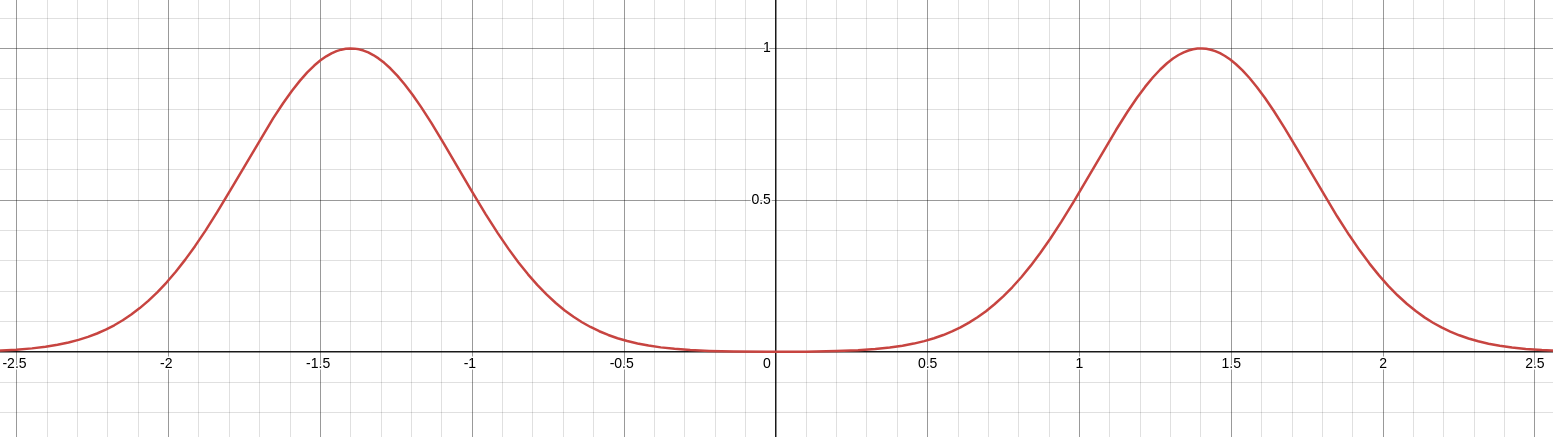
\includegraphics[width=0.9\textwidth]{fig/part-1/densi_spec_sym}
	\caption{Exemple de densité spectrale d'un signal réel \textbf{ESP A 1,4}}
	\label{fig:densi_spec_sym}
\end{figure}
\\
Même problème avec la covariance : sachant l'égalité des deux notions de fréquences moyenne (\cref{eq:esp_freq}, \cref{prop:mom_freq}), on peut définir la covariance temps-fréquence d'un signal $x$ par :
\begin{align*}
	\text{Cov}(x) \defeq \text{Cov}\big(t,\phi'(t) \big) 
	&= \esp[\densit]{t\phi'(t)} - \esp[\densit]{t} \esp[\densit]{\phi'(t)} \\
	&= \esp[\densit]{t\phi'(t)} - \esp[\densit]{t} \esp[\densis]{\nu}	
\end{align*}
\\
Ce coefficient est sensé mesurer une corrélation entre l'évolution d'un signal au cours du temps avec ses fréquences. S'il est réel, alors  $\text{Cov}(x)$ sera toujours nulle ; de là à en conclure que la fréquence instantanée de n'importe quel signal (réel) est toujours décorrélée du temps serait, pour le moins, insatisfaisant.
\\

Pour résoudre le problème, une méthode consiste à construire un nouveau signal $\SA{x}$ en supprimant les fréquences négatives de $x$ :
\[\mathcal{F}\big[\SA{x}\big] = 2\one_{\R^+}\fou{x}\]
où $\one_E$ est la fonction indicatrice sur l'ensemble $E$ et où le facteur 2 assure la conservation de l'énergie du signal. Cela mène à la définition :

\begin{definition}[Transformée de Hilbert et en SA]\label{def:transfo_sa&hilbert}
	On appelle \emph{transformé de Hilbert de} $x$, l'application :
	\begin{equation}\label{eq:transfo_Hilb}
		\mathcal{H}[x] :\ \begin{aligned} 
			\R \quad &\lr\qquad\quad \C \\	
			t\quad &\longmapsto\ \frac{1}{\pi}\fint_\R \frac{x(s)}{t-s}ds %=  \frac{1}{\pi}\left(\vpC\right)*x
		\end{aligned}
	\end{equation}
	où l'intégrale barré représente la \emph{valeur principale de Cauchy} (voir \cref{ann:transfo_SA} pour plus de détail) :
	\begin{align*}
		\fint_\R \frac{x(s)}{t-s}ds &\defeq \lim_{\varepsilon\lr0^+} \int_{-\infty}^{-\varepsilon} \frac{\varphi(t)}{t}dt + \int_{+\varepsilon}^{+\infty} \frac{\varphi(t)}{t}dt 
		%\\ &= \int_0^{+\infty} \frac{\varphi(t) - \varphi(-t)}{t}dt
	\end{align*}
	Avec, on définit la \emph{transformée en signal analytique} (SA) de tout signal $x$ comme l'unique application $\SA{x}$ telle que $\ \Fou{\SA{x}\big.}= 2\one_{\R^+}\fou{x}$. Elle est donnée par la formule :
	\begin{equation}\label{eq:transfo_SA}
		\SA{x} :\ \begin{aligned} 
			\R \quad &\lr\qquad\quad \C \\	
			t\quad &\longmapsto\ x(t) + i\mathcal{H}[x](t) %= x(t) + \frac{i}{\pi}\fint_\R \frac{x(s)}{t-s}ds
		\end{aligned}
	\end{equation}
	Plus généralement, tout signal dont le spectre est à support dans $\R^+$ sera dit \emph{analytique}.
\end{definition}
\skipl

Pour mieux comprendre ce que fait la transformation en signal analytique, revenons sur la notion de fréquence instantanée pour les signaux réels.
%Par souci de commodité, plutôt que redéfinir tout le vocabulaire développé plus haut (fréquence moyenne, temps moyen, \etc) pour les signaux réel via la transformation $\mathcal{A}$, dans la suite du mémoire on travaillera directement avec $\SA{x}$. %^(et on verra que c'est essentiel).
\\



\subsection{Interprétabilité de la transformée en SA}\label{sec:Bedrisan&AM-FM}

Pour définir l'amplitude et la phase instantanée d'un signaux réel, on par a nouveau du cas le plus simple. Si $x$ est un signal pur, il va s'écrire :
\[x(t) = a \cos(2\pi\nu t + \varphi),\qquad a,\nu,\varphi\in\R\]
\\
Pour généraliser cette écriture, il suffit donc de poser les amplitude et phase instantanée $a$ et $\phi$ telles que :
\[x(t) = a(t) \cos\big( \phi(t) \big)\]
\\
Contrairement au cas complexe, ici la pair $(a,\phi)$ n'est pas unique et pour contraindre ce choix, on s'appuie sur la transformée $\SA{x}$. Sachant que, dans le cas $x(t)\in\R$, la transformée de Hilbert est à valeur dans $\R$ (intégrale d'une fonction réelle), on a :
\[\SA{x}(t) = a(t)e^{i\phi(t)}\quad \Lr\quad \left\{\begin{aligned}x(t) &= \Re e \SA{x} = a(t) \cos\phi(t) \\ \mathcal{H}[x](t) &= \Im m \SA{x} = a(t) \sin\phi(t)
\end{aligned}\right.\]
\\
D'où la définition :
\begin{definition}[Amplitude et phase instantanée]\label{def:ampli-phase_instant}
	L'\emph{amplitude instantanée} $a_x$ et la \emph{phase instantanée} $\phi_x$ de tout signal $x$ réel sont définies comme étant respectivement l'amplitude et la phase de $\SA{x}$ :
	\begin{align}\label{eq:ampli-phase_instant}
		a_x &= \big|\SA{x}\big|   &   \phi_x &= \arg\big(\SA{x}\big)
	\end{align}
	De même, les \emph{impulsion} et \emph{fréquence instantanée} sont données par $\ \phi'_x\ $ et $\ \nicefrac{1}{2\pi}\phi_x'$.
\end{definition}
\skipl

Si un signal est présenté sous la forme  $\ x=a\cos\phi$, rien n'implique que $a$ et $\phi$ correspondent bel et bien à l'amplitude et la phase instantanée. Si ce n'est pas le cas, c'est que cette décomposition n'est ``pas la bonne'', en cela qu'elles ne s’interprètent pas comme l'on aimerait.
\\
Aussi, quand bien même $x$ peut toujours être écrit comme partie réel de sa transformé en SA, cette écriture n'est nécessairement toujours satisfaisante. Pour le comprendre, détaillons le cas où $x$ s'écrit comme produit de deux signaux pures (\cref{fig:exemple_tSA_1/2}) :
\[x_1(t) = \cos (2\pi\nu_1t)\cos (2\pi\nu_2t)\]

\begin{figure}[h]\centering
	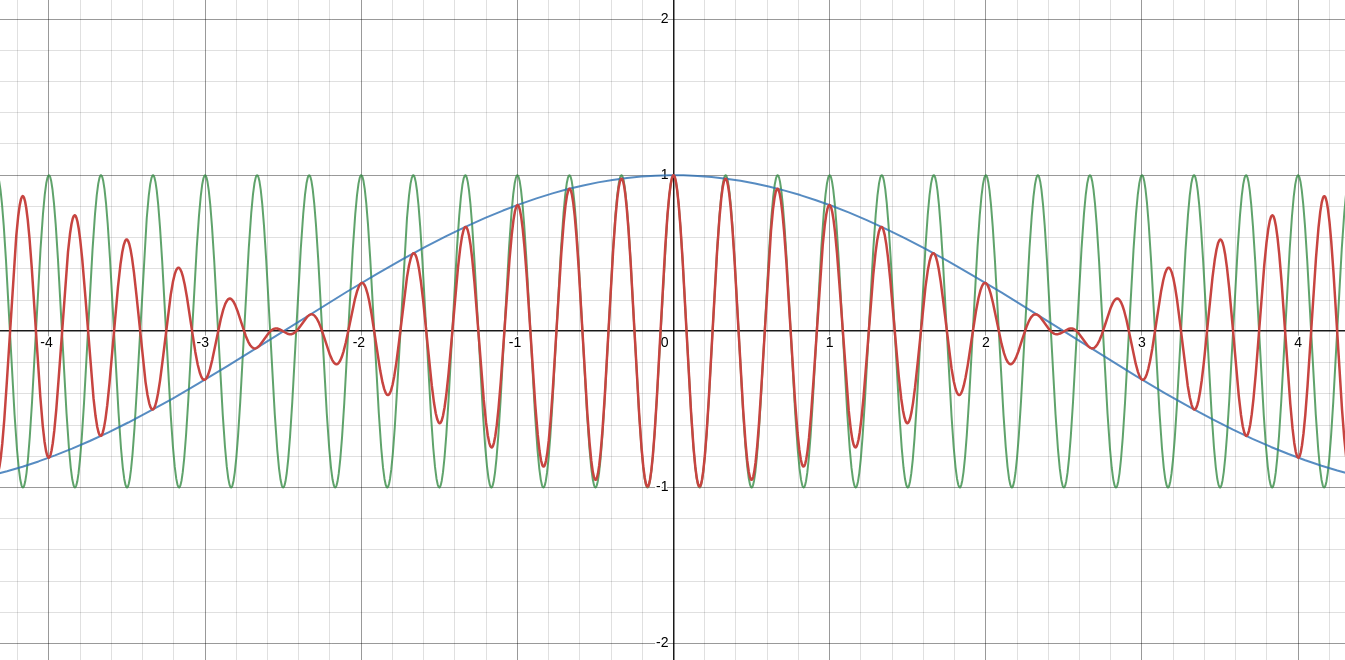
\includegraphics[width=0.48\textwidth]{fig/part-1/ex SA - 11.png}
	\hfill
	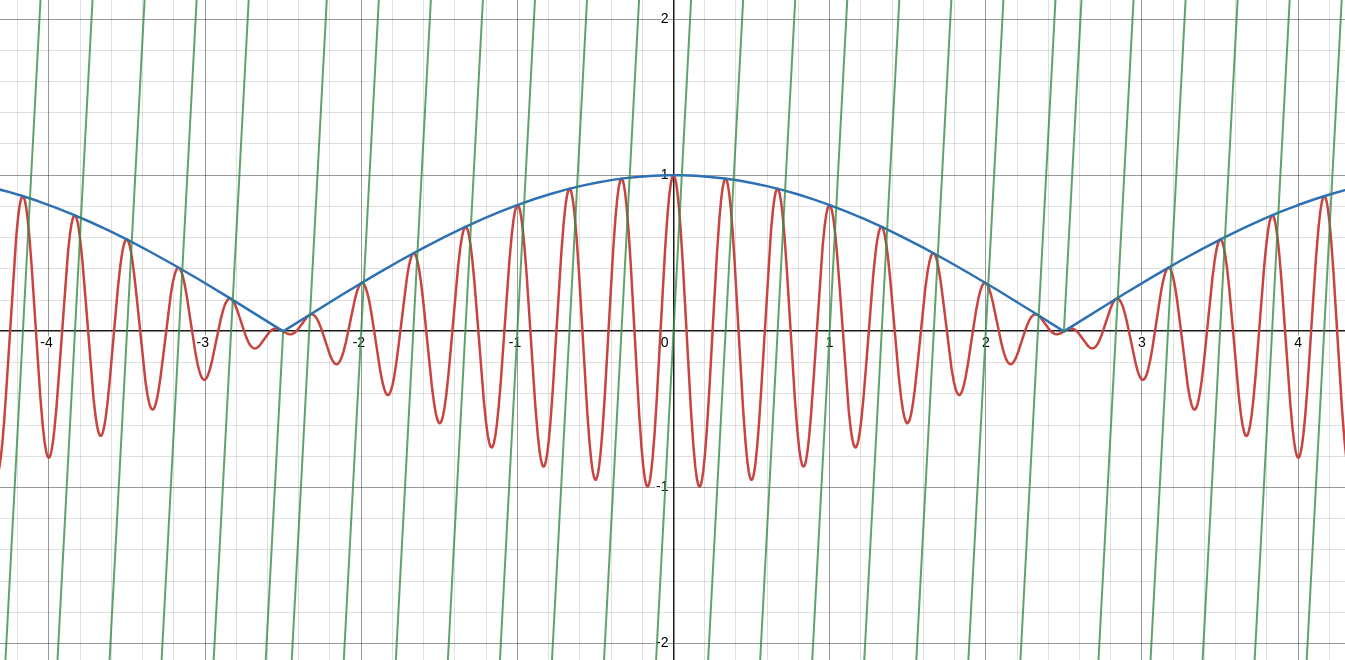
\includegraphics[width=0.48\textwidth]{fig/part-1/ex SA - 12.png}
	\caption{Représentation graphique du signal $x$ (rouge) avec $\nu_1=3$ et $\nu_2=0.1$. Sur l'image de gauche, avec signaux de fréquences pures (bleu et vert). Sur l'image de droite, avec son amplitude (bleu) et sa phase instantanée (vert). Les discontinuités de la phase sont dû à l'arrondi à $2\pi$  près de l'argument de $\SA{x_1}$ et à la façon dont il est calculé lorsque le signal s'annule (mise à 0). Voir \href{https://www.desmos.com/calculator/gcedcdfkhr}{ici} pour un graphique dynamique.}
	\label{fig:exemple_tSA_1/2}
\end{figure}

\noindent
On montre sans mal\footnote{\itshape
	$\fou{x}_1$ est donné par 4 Diracs, en ne gardant que ce non nul sur $\R^+$ on obtient le spectre de $\SA{x_1}$ et il reste plus qu'à inverser la transformée de Fourier.}
que si $\ \nu_1\geq\nu_2$, alors la transformée en SA de $x_1$ s'écrit :
\[\SA{x_1} = \cos \left(2\pi\nu_2 t\right) e^{2\i\pi\nu_1 t}\]
\\
Le signal $\SA{x_1}$ n'est ici pas sous forme exponentielle à proprement parler puisque le cosinus peut être négatif (pour s'y ramener, il suffit de passer le cos en valeur absolue et d'ajouter $\pi$ à l'argument lorsque nécessaire) mais l’avantage de cette forme est qu'elle fait clairement apparaître les fréquences $\nu_{1,2}$. En particulier, la fréquence instantanée du signal est la plus grandes des deux fréquences $\nu_1$ et $\nu_2$. La plus petite, elle, se retrouve dans l'amplitude. 
\\
Ce résultat est rassurant en cela qu'il est plus naturel de voir le cosinus de basse fréquence comme modulant celui de haute fréquence que l'inverse comme on le voit sur la première image de la figure \ref{fig:exemple_tSA_1/2}. 
\\
Aussi, en mettant les hautes fréquences du signal dans la fréquence instantanée, on s'assure de limiter les variations de l'amplitude. Cela apporte bien plus de contrainte en terme de décomposition $(a_{x_1},\phi_{x_1})$, en cela qui si l'inverse étant vrai, alors toute les fréquences pourrait être envoyé dans l'amplitude, ce qui laisserait la phase invariante.
\\

Cela étant dit, lorsque l'on fait varier $\nu_1$ et $\nu_2$, le résultat n'est pas toujours si intuitif. C'est notamment le cas lorsque les deux deviennent de plus en plus proche :

\begin{figure}[h]\centering
	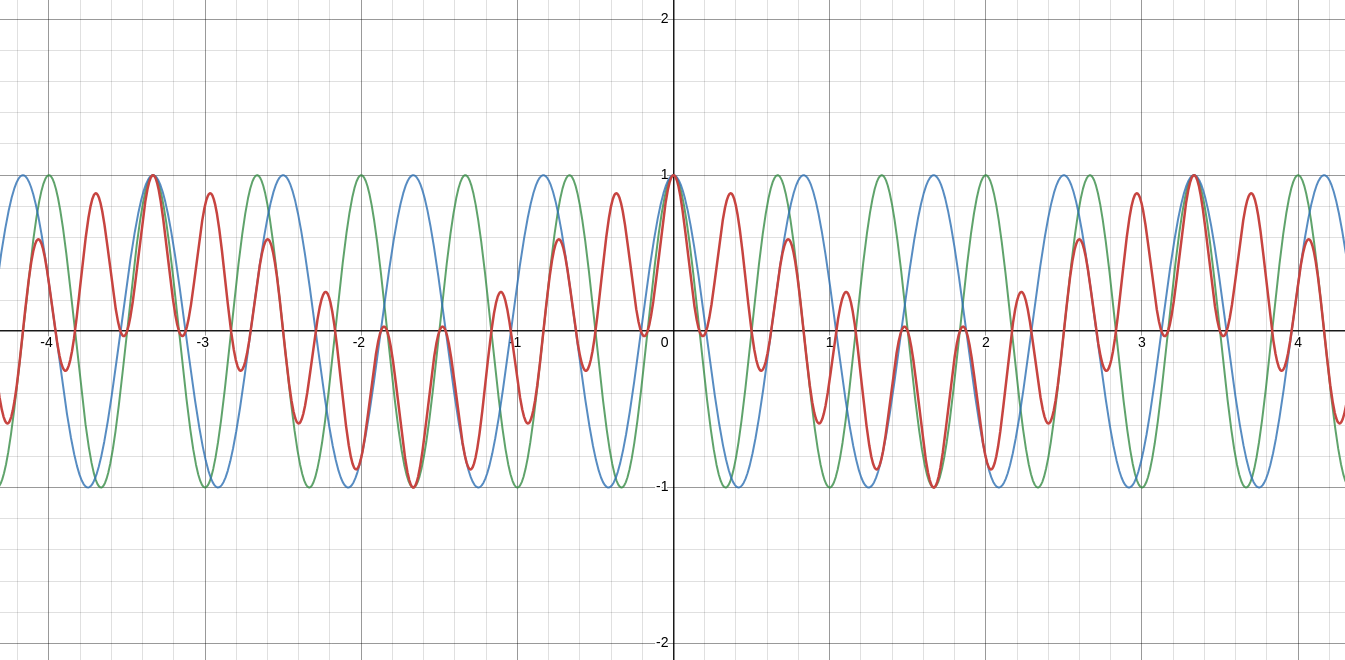
\includegraphics[width=0.48\textwidth]{fig/part-1/ex SA - 21.png}\hfill
	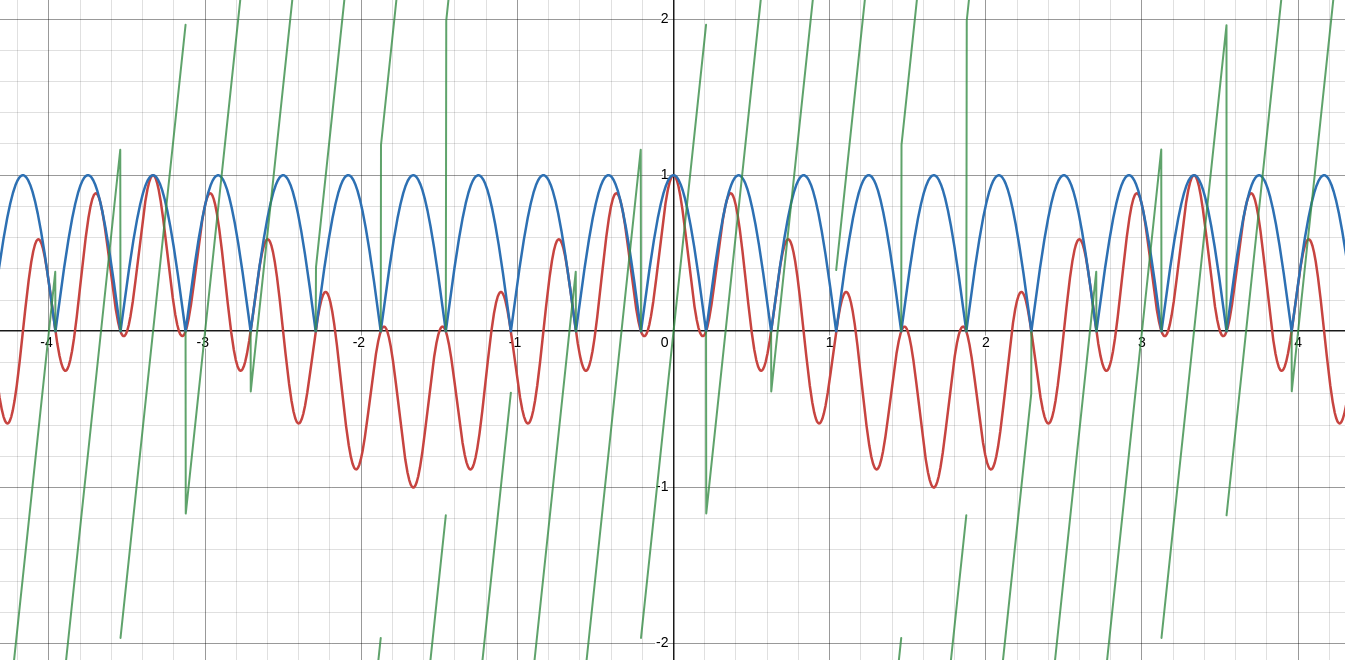
\includegraphics[width=0.48\textwidth]{fig/part-1/ex SA - 22.png}
	\caption{Idem que pour la figure \ref{fig:exemple_tSA_1/2} précédente, avec cette fois $\nu_1=1.5$ et $\nu_2=1.3$.}
	\label{fig:exemple_tSA_2/2}
\end{figure}

Pour comprendre pourquoi l'amplitude ne fait pas ce qu'on attendrait d'elle, est introduit le théorème de Bedrosian :

\begin{theoreme}[de Bedrosian]\label{theo:2Bedrosian}
	Dans sa formulation la plus générale, le théorème de Bedrosian énonce que si deux fonctions $f,g\in L^2(\R)$ sont telles l'une des trois assertions suivantes est vraie :
	\begin{itemize}%[label=\textit{\arabic*}. ]
		\item 
		\item $\exists \lambda\in\R^+\ |\ \supp \fou{f} \subset [-\lambda, +\infty[,\ \supp \fou{g} \subset [\lambda, +\infty[$\label{item:1condi_theo2Bedrosian}
		
		\item $\exists \lambda\in\R^+\ |\ \supp \fou{f} \subset ]-\infty, \lambda],\ \supp \fou{g} \subset ]-\infty,-\lambda]$ \label{item:2condi_theo2Bedrosian}
		
		\item $\exists (\lambda_1,\lambda_2)\in \R^+\times\R^+ \setminus\{(0,0)\}\ |\ \supp \fou{f} \subset [-\lambda_1, \lambda_2],\ \supp \fou{g} \subset \R\setminus[-\lambda_2,\lambda_1]$
		
	\end{itemize}
	alors la transformée de Hilbert de leur produit s'écrit (voir \cite{wang_simple_2009} pour une démonstration) :
	\begin{equation}\label{eq:2Bedrosian}
		\hilb{fg} = f\hilb{g}
	\end{equation}
\end{theoreme}

Dans le cas d'un signal réel, suivant la \cref{def:ampli-phase_instant} on peut écrire $\ x=a_x\cos \phi_x$.
Comme $a_x$ et $\cos \phi_x$ sont réelles, seule la troisième condition du théorème de Bedrosian peut être satisfaite pour peu que $\lambda_1=\lambda_2$. Ainsi :

\begin{corollaire}\label{coro:AM-FM}
	Toujours avec les même notations, si $a_x\in L^2(\R)$, $\cos\phi_x\in L^2(\R)$ et qu'il existe $\lambda\in\R^{+_*}$ tel que :
	\begin{equation}\label{eq:condi_AM-FM}
		\supp \Fou{a_x} \subset [-\lambda, \lambda],\quad \supp \Fou{\cos\phi_x} \subset \R\setminus[-\lambda,\lambda]
	\end{equation}
	Alors on a :
	\begin{align}\label{eq:result_AM-FM}
		\hilb{x} &= a_x\hilb{\cos \phi_x}  &  \qquad\qquad&\text{et si }a_x(t)\neq 0,  &  \hilb{\cos \phi_x}(t) = \sin\phi_x(t)
	\end{align}
\end{corollaire}
\skipl

Pour interpréter ce \namecref{coro:AM-FM}, prenons un autre exemple : $\ x_2(t) = a(t)\cos(2\pi \nu_0 t)$. Sa transformé de Fourier est donnée par :
\begin{align*}
	\fou{x}_2(\nu) &= \fou{a}(\nu)*\frac{1}{2}\Big(\delta(\nu-\nu_0) + \delta(\nu+\nu_0)\Big) \\
	&= \frac{1}{2}\Big(\fou{a}(\nu+\nu_0) + \fou{a}(\nu-\nu_0)\Big)
\end{align*}
\\
Graphiquement, la transformé de Fourier de $x_2$ duplique le graphe de $\fou{a}$ en $\pm\nu_0$ et somme les deux. La condition \eqref{eq:condi_AM-FM} du \cref{coro:AM-FM} demande alors que $\nu_0$ soit choisie de telle sorte que :
\[\supp \Fou{a}\subset[-\nu_0, \nu_0]\]
\\
C'est-à-dire qu'il n'y ait pas de chevauchement entre les deux courbes $\ \Gamma_\pm : \nu \longmapsto \fou{a}(\nu\mp\nu_0) $ (voir \cref{fig:alising-ish} ci-dessous). Moralement, cela assure qu'en ne prenant que la partie positive du spectre de $x_2$, l'on ne ramène pas avec une partie de $\fou{a}(\nu+\nu_0)$. Quant bien même cette explication est simpliste puisqu'ici $\phi$ est linaire, on peut voir que le phénomène est finalement très proche de celui d'aliasing.
\\

\begin{figure}[h]\centering
	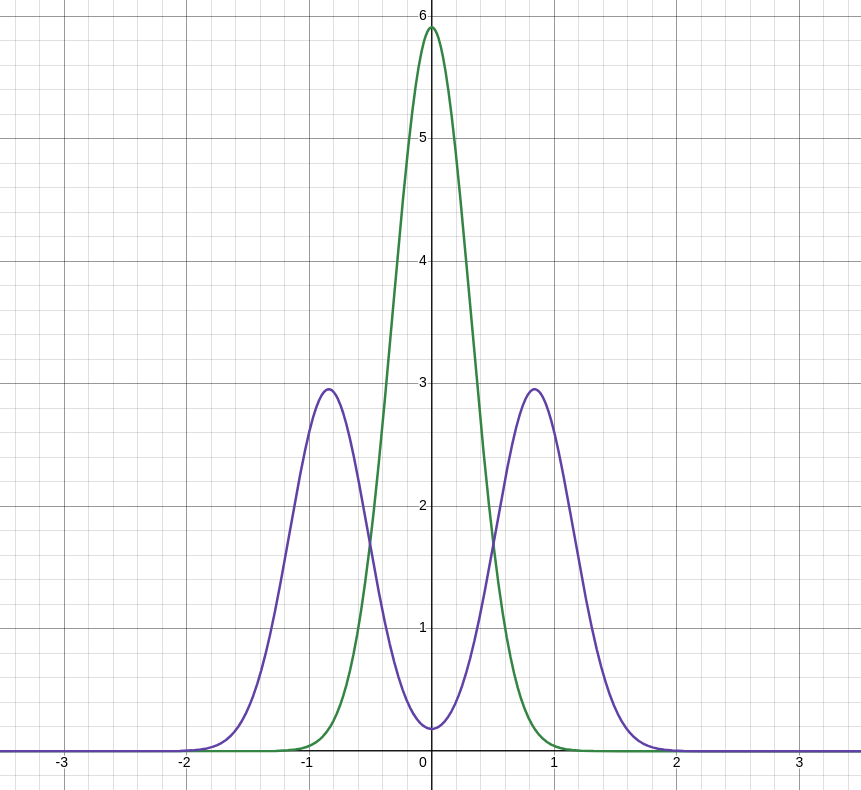
\includegraphics[width=0.45\textwidth]{fig/part-1/bedro condi 1.png} 
	\hfill
	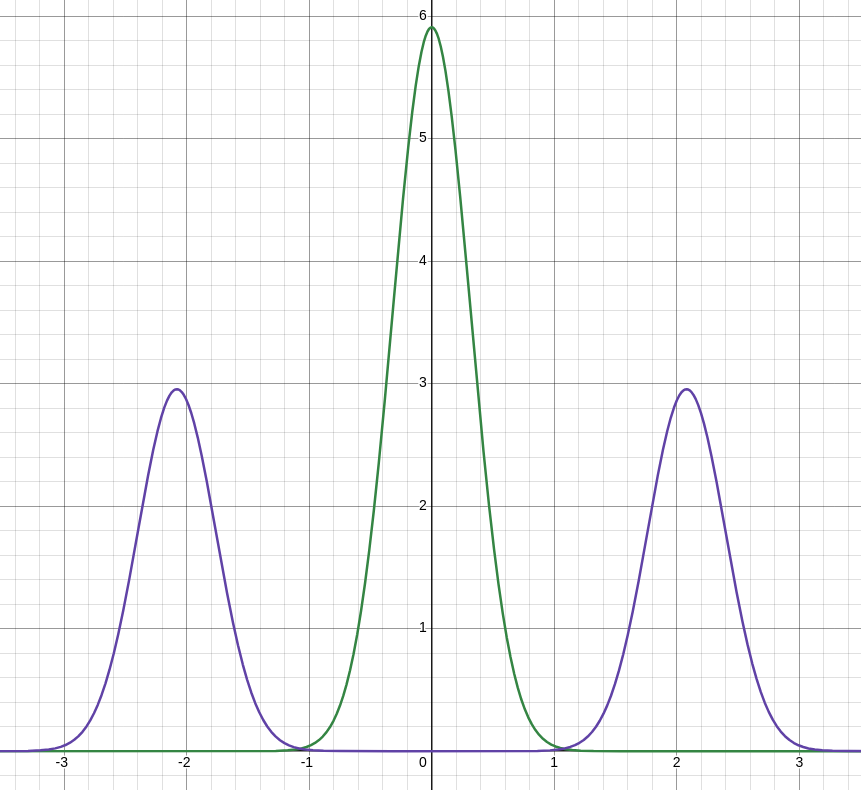
\includegraphics[width=0.45\textwidth]{fig/part-1/bedro condi 2.png} 
	\caption{Sur les deux graphiques sont représentés en vert $\fou{a}$ et en violet $\fou{x}_2$. Dans le premier cas l'hypothèse de Bedrosian et respectée mais pas dans le second.}
	\label{fig:alising-ish}
\end{figure}


Pour revenir sur l'exemple $x_1$ précédent, dans la seconde figure \ref{fig:exemple_tSA_2/2}, l'amplitude ne colle plus à l'interprétation que l'on voudrait justement parce que la condition de Bedrosian n'est plus respecter (à savoir $\nu_1\geq 2\nu_2$). 
\\
Formellement, \textbf{JE COMPRENDS TOUJOURS PAS COMMENT CA POSE PROBLEME DANS LA DEFINITON / INTERPRETATION DE $\bf{\SA{x}}$ ! HHHHHH !!!}
\\



\section{Généralisation aux signaux multivariés}\label{sec:sign_multivar}

Maintenant que les paramètres instantanée sont proprement définie pour les cas réel et complexe, qu'en est il des signaux multivariés :

\begin{definition}[Signal multivarié]\label{def:signal_multivar}
	Un \emph{signal multivarié}, ou \emph{$n-$varié}, est un vecteur composé de $n\in\N^*$ signaux $x_i$. Pour $n=2$ (resp.$=3$), on parle de signal \emph{bivarié} (resp. \emph{trivarié}).
	\\
	Dans la continuité de ce qui à été dit dans lplus tôt, dans le cas des signaux réels, on s'intéressera au vecteur composé des transformées en SA (eq. \eqref{eq:transfo_SA}, déf. \ref{def:transfo_sa&hilbert}) des $x_i$.
	%\textbf{Au moins dans toute cette \namecref{sec:sign_multivar}}, un tel signal sera noté :
	%\[\sa{x}(t)\ :\quad \begin{aligned} 
	%	\R\quad &\lr\qquad \C^n \\t\quad &\longmapsto\ \begin{pmatrix} \mathcal{A}[x_1] \\ 
	%		\mathcal{A}[x_2] \\ \vdots \\ \mathcal{A}[x_n] \end{pmatrix}
	%\end{aligned} \]
	\\
	On supposera que chaque composante $x_i$ de $\bf{x}$ aura autant de régularité et de condition d'intégrabilité que nécessaire \textbf{(il vaudra préciser lesquelles éventuellement)}.
\end{definition}




\subsection{Phase et fréquence instantanée de signal multivarié }\label{sec:param_instant_nvar}

Afin de contraindre ce choix, on s'inspire propriétés de la phase instantanée vu plus tôt pour en déduire deux approches :
\begin{itemize}
	\item D'une part, l'espérance de la fréquence instantanée (ici vu comme dérivée à $2\pi$ près de la phase\footnote{\itshape
		La pertinence de cette définition dans le cas multivarié sera discuté plus loin... \textbf{or is it ? (si oui, dis cref où)}})
	doit donnée la fréquence moyenne au sens de Fourier, eq. \eqref{eq:esp_freq}.
	
	\item D'autre part, les conditions d'interprétation \eqref{eq:condi_AM-FM} de la décomposition $(a_x,\phi_x)$, \cref{coro:AM-FM}, exige que les hautes fréquences du signal se retrouve dans la phase.
\end{itemize}

Pour cela on introduit les notations utiles au cas multivarié :
\begin{definition}[densité d’énergie]\label{def:densi_dE-mv}
	Étant donné un signal multivarié $\bf{x}=(x_i)_{1\leq i\leq n}$, les densités d'énergie de chaque composante $x_i$  sont notées :
	\begin{align}\label{eq:densi_dEi}
		\densit_i\ &:\quad \begin{aligned}\R\ &\lr\quad \R^+ \\ t\ &\longmapsto\ \big|x_i(t)\big|^2 = a(t)^2 a_i(t)^2 \end{aligned}  
		&
		\densis_i\ &:\quad \begin{aligned}\R\ &\lr\quad \R^+ \\ \nu\ &\longmapsto\ \big|\fou{x}_i(\nu)\big|^2 \end{aligned}
	\end{align}
	Et les densités d'énergies associées au signal $\bf{x}$ complet :
	\begin{align}\label{eq:densi_dE-mv}
		\densit\ &:\quad \begin{aligned}\R\ &\lr\quad \R^+ \\ t\ &\longmapsto\ \big\|\bf{x}(t)\big\|^2 = \sum_{i=1}^n \densit_i(t) \end{aligned}  
		&
		\densis\ &:\quad \begin{aligned}\R\ &\lr\quad \R^+ \\ \nu\ &\longmapsto\ \big\|\fou{\bf{x}}(\nu)\big\|^2 = \sum_{i=1}^n \densis_i(t) \end{aligned}	
	\end{align}
\end{definition}
\skipl

La première approche, inspiré de \cite{cano_mathematical_2022} consiste donc de reprendre le ``calculation trick'' \eqref{eq:moment_f}, pour en déduire la fréquence moyenne :
\begin{align*}
	\esp[\densis]{\nu} = \int_\R \nu\densis(\nu)d\nu &= \int_\R \nu\sum_{i=1}^n \densis_i(\nu) d\nu \\
	&= \sum_{i=1}^n\esp[\densis_i]{\nu} \\
	&= \sum_{i=1}^n\frac{1}{2\pi}\int_\R \phi_i'(t)\densit_i(t)dt \\
	&= \frac{1}{2\pi}\int_\R a(t)^2\sum_{i=1}^n\phi_i'(t)a_i(t)^2 dt 
	\\ &= \frac{1}{2\pi} \esp[\densit]{\sum_{i=1}^n \phi_i'{a_i}^2}
\end{align*}
\\
Ce qui mène à une première (potentielle) définition de la phase instantanée :
\begin{equation}\label{eq:phas_inst_v1}
	\phi = \int \sum_{i=1}^n \phi_i'(s){a_i}(s)^2ds 
	= \sum_{i=1}^n \int \phi_i'(s){a_i}(s)^2ds 
	%= \sum_{i=1}^n \esp[\nicefrac{\densit_i}{\densit}]{\phi_i'}
\end{equation}
\\

La seconde approche, fortement inspirée par les travaux de Lilly \& Olhede  \cite{lilly_analysis_2012}, se base sur l'idée de séparation haute/basse fréquences du signal $\bf{x}$. Pour cela, l'on commence par faire apparaître la phase $\phi$ --- pour l'instant inconnue --- en écrivant $\bf{x}$ sous la forme :
\[\forall t\in\R,\qquad \bf{x}(t) = e^{i\phi(t)} e^{-i\phi(t)} \bf{x}(t) \defeq e^{i\phi(t)} \bf{y}(t)\]
\\
Si $\phi$ est bien choisie, alors $\bf{y}$ ne devrait contenir que les informations associées à l'amplitude et la polarisation de $\bf{x}$. Or, la phase doit contenir les hautes fréquences du signal. 
Pour s'en assurer on demande, à l'inverse, que les basses fréquences du signal soient données par $\bf{y}$ en limitant ces variations. Concrètement, $\phi$ doit être choisie de sorte à minimiser la dérivée $\dot{\bf{y}}'$ :
\[\forall t\in\R,\qquad \phi(t) = \argmin{\theta(t)}{\big\|\dot{\bf{y}}(t)\big\|_2}^2 = \argmin{\theta(t)}{\Big\|e^{-i\theta(t)}\big(\dot{\bf{x}}(t) - i\theta(t)'\bf{x}(t)\big)\Big\|_2}^2 = \argmin{\theta(t)}{\big\|\dot{\bf{x}}(t) - i\theta'(t)\bf{x}(t)\big\|_2}^2\]
\\
La contrainte ne dépendant que de la dérivée $\theta'$, on se ramène à :
\[\min_{\theta(t)}{\|\dot{\bf{y}}(t)\|_2}^2 = \min_{\theta'(t)}{\big\|\dot{\bf{x}}(t) - \theta'(t) \bf{x}(t)\big\|_2}^2\]
\\
En rappelant que $\frac{d}{dx}{\big\|f(x)\big\|_2}^2 = 2\Re e\big\langle f(x), f'(x)\big\rangle$, il vient que ce minimum\footnote{\itshape
	L'extremum obtenu est l'unique minimum globale puisque $t\longmapsto \|at + b\|^2$ est strictement convexe pour $a\neq0$.}
est atteint par $\phi'(t)$ à condition que :
\begin{align*}
	\frac{d}{d\phi'}{\big\| \dot{\bf{x}} - i\phi' \bf{x}\big\|_2}^2 = 0 \quad \Llr\quad
	0 &= 2\Re e\left\langle  \dot{\bf{x}} - i\phi' \bf{x} ,  \frac{d}{d\phi'}\big(\dot{\bf{x}} - i\phi' \bf{x}\big)\right\rangle \\
	&= 2\Re e\big\langle  \dot{\bf{x}} - i\phi' \bf{x} ,  - i \bf{x}\big\rangle \\
	&= 2\Re e\Big(i\big\langle  \dot{\bf{x}} ,  \bf{x}\big\rangle\Big) + 2\phi'\Re e\big\langle   \bf{x} ,  \bf{x}\big\rangle\\
	&= -2\Im m\big\langle  \dot{\bf{x}} ,  \bf{x}\big\rangle + 2\phi'{\| \bf{x}\|_2}^2
\end{align*}
Ainsi :
\begin{align}\label{eq:phas_inst_v2}
	\phi' &= \frac{\Im m\big\langle  \dot{\bf{x}} ,  \bf{x}\big\rangle}{{\| \bf{x}\|_2}^2} = \frac{-\Im m\big\langle  \bf{x},  \dot{\bf{x}}\big\rangle}{{\| \bf{x}\|_2}^2}  &  &\text{et}  &  \phi &= -\Im m\int \frac{\big\langle \bf{x}(s) , \dot{\bf{x}}(s) \big\rangle}{\|\bf{x}(s)\|^2} ds
\end{align}
\\
Ce qui, sous forme exponentiel, se réécrit :
\begin{align*}
	-\Im m\frac{\big\langle \bf{x}(t) , \dot{\bf{x}}(t) \big\rangle}{\|\bf{x}(t)\|^2} &= -\Im m\frac{1}{a(t)^2} \sum_{i=1}^n a(t)a_i(t)e^{i\phi_i(t)}\congu{\Big( \big(aa_i\big)'(t) +a(t)a_i(t)i\phi_i'(t)\Big)e^{i\phi_i(t)}} \\
	&= -\Im m\frac{1}{a(t)^2} \sum_{i=1}^n a(t)a_i(t)\big(aa_i\big)'(t) -ia(t)^2a_i(t)^2\phi_i'(t) \\
	&= -\frac{1}{a(t)^2} \sum_{i=1}^n -a(t)^2a_i(t)^2 \phi_i'(t) \\
	&= \sum_{i=1}^n a_i(t)^2 \phi_i'(t)
\end{align*}
Soit la même expression que \eqref{eq:phas_inst_v1} obtenue par le premier raisonnement :
\[-\Im m\int \frac{\big\langle \bf{x}(s) , \dot{\bf{x}}(s) \big\rangle}{\|\bf{x}(s)\|^2} ds = \int \sum_{i=1}^n a_i(s)^2 \phi_i'(s) = \sum_{i=1}^n \int a_i(s)^2 \phi_i'(s)ds\]
\\
Cela justifie la définition :

\begin{definition}[Phase dynalique/instantanée] \label{def:phase_d}
	\'Etant donné un signal $\bf{x}\in \conti{\R}{\C^n}$ quelconque, on appelle \emph{phase instantanée} ou \emph{dynamique} à l'instant $t$ partant du $t_0$, le réel :
	\begin{equation} \label{eq:phase_d}
		\forall t_0, t\in\R, \quad \phased(\bf{x}, t_0,t) \defeq -\int_{t_0}^t \frac{\Im m \big\langle \bf{x}(s) , \dot{\bf{x}}(s) \big\rangle}{\|\bf{x}(s)\|^2} ds =\sum_{i=1}^n \int_{t_0}^t a_i(s)^2 \phi_i'(s)ds
	\end{equation}
	On s'autorisera à omettre les paramètres de $\phased$ lorsque cela ne prête pas à confusion.
\end{definition}
\skipl

Le terme ``dynamique'' viens, entre autre, du fait que dans son cadre d'étude habituelle, la dérivée $\dot{\bf{x}}$ se voit remplacé par un hamiltonien $h\bf{x}$, voir par exemple \cite[sec. 2]{bohm_geometric_2003}, \cite[p.~215]{mukunda_quantum_1993}. En particulier, en mécanique quantique, cet hamiltionien régie l'équation de Schödinger :
\begin{equation}\label{eq:schrodinger}
	i\frac{d \psi(t)}{dt} = h\psi(t)
\end{equation}

Sachant que $\bf{x}$ n'a aucune raison de suivre une telle équation dans notre cas, poser $h = i\frac{d}{dt}$ enlève toute contrainte. On retrouve ainsi, modulo un jeu de convention sur le produit hermitien, la formule \eqref{eq:phase_d} ci-dessus.
\\ Notons enfin qu'une fois la phase dynamique ``extraite'' de $\bf{x}$, le vecteur restant $\bf{y}$ n'a évidement pas de phase dynamique, ce qui se traduit par la formule :

\textbf{... un peu plus de blabla pour faire transition sur la suite ...}





\begin{annexe}
	
\section{Complément sur l'analyse temps-fréquence} 

\subsection{Un bon moment...}\label{ann:integ_trick}

Pour montrer les formules de la \cref{prop:mom_freq}, on commence par montrer ce que Cohen \cite{cohen_time_1995} appelle les  :

\begin{lemme}[``Calculation tricks''] \label{prop:integ_trick}
	Si le signal est $n$ fois dérivable et que la densité d’énergie spectrale associée $\densis$ admet un moment d'ordre $n$, alors ce moment est donnée par la formule :
	\begin{equation}\label{eq:moment_f}
		\forall n\in\N,\qquad \esp[\densis]{\nu^n} = \left(\frac{i}{2 \pi}\right)^n  \int_\R x(t) \frac{d^n}{dt^n} \congu{x(t)} dt = \left(\frac{i}{2 \pi}\right)^n  \left\langle x, \frac{d^n}{dt^n}x\right\rangle
	\end{equation}
	\\
	Avec les hypothèses analogues, les moments de $\densit$ s'écrivent :
	\begin{equation}\label{eq:moment_t}
		\forall n\in\N,\qquad \esp[\densit]{t^n} = \left(\frac{1}{2i \pi}\right)^n  \int_\R \fou{x}(\nu) \frac{d^n}{dt^n} \congu{\fou{x}(\nu)} dt = \left(\frac{1}{2i \pi}\right)^n  \left\langle \fou{x}, \frac{d^n}{d\nu^n}\fou{x}\right\rangle
	\end{equation}
\end{lemme}


\begin{demo}[du \cref{prop:integ_trick}]
	\`A supposer que les intégrales existes et que le théorème de Fubini s'applique, on a $\forall n\in\N$ :
	\begin{align*}
		\esp[\densis]{\nu^n} = \int_\R \nu^n\densis(\nu) d\nu &= \int_\R \nu^n \fou{x}(\nu)\congu{\fou{x}(\nu)} d\nu \\
		&= \int_\R \nu^n \int_\R x(t)e^{-2i \pi \nu t} dt \int_\R \congu{x(t')}e^{2i \pi \nu t'} dt' d\nu \\
		&= \int_\R \int_\R x(t) \congu{x(t')} \int_\R \nu^n e^{-2i \pi \nu (t-t')} d\nu dt dt' 
	\end{align*}
	Ici, on remarque que :
	\begin{align*}
		\nu^n e^{-2i \pi \nu (t-t')} &= \nu^{n-1}\frac{1}{-2i \pi}\frac{d}{dt}e^{-2i \pi \nu(t-t')} \\
		&= \nu^{n-2}\frac{1}{(-2i \pi)^2}\frac{d^2}{dt^2}e^{-2i \pi \nu(t-t')} \\
		&\ \vdots \\
		&= \frac{1}{(-2i \pi)^n}\frac{d^n}{dt^n}e^{-2i \pi \nu(t-t')}
	\end{align*}
	\\
	
	En jouant sur les ordres d'intégrations, on obtient :
	\begin{align*}
		\esp[\densis]{\nu^n} &= \int_\R \int_\R x(t) \congu{x(t')} \int_\R \nu^n e^{-2i \pi \nu (t-t')} d\nu dt dt'  \\
		&= \int_\R \int_\R x(t) \congu{x(t')} \int_\R \frac{1}{(-2i \pi)^n}\frac{d^n}{dt^n}e^{-2i \pi \nu(t-t')} d\nu\, dt\, dt' \\
		&= \frac{1}{(-2i \pi)^n} \int_\R \int_\R x(t) \congu{x(t')} \frac{d^n}{dt^n}\int_\R e^{-2i \pi \nu(t-t')} d\nu\, dt\, dt' \\
		&= \left(\frac{1}{-2i \pi}\right)^n \int_\R \int_\R x(t) \congu{x(t')} \frac{d^n}{dt^n}\mathcal{F}\big[1\big](t-t') dt\, dt'
	\end{align*}
	La transformée de Fourier de 1 est un dirac, il vient, modulo quelques jeux d'ordre d'intégration :
	\begin{align*}
		\esp[\densis]{\nu^n} &= \left(\frac{1}{-2i \pi}\right)^n \int_\R \int_\R x(t) \congu{x(t')} \frac{d^n}{dt^n}\mathcal{F}\big[1\big](t-t') dt\, dt' \\
		&= \left(\frac{i}{2 \pi}\right)^n \int_\R \int_\R x(t) \congu{x(t')} \frac{d^n}{dt^n}\delta(t-t') dt\, dt' \\
		&= \left(\frac{i}{2 \pi}\right)^n \int_\R x(t) \int_\R \congu{x(t')} \frac{d^n}{dt^n}\delta(t-t') dt' dt \\
		&= \left(\frac{i}{2 \pi}\right)^n \int_\R x(t) \frac{d^n}{dt^n} \int_\R \congu{x(t')} \delta(t-t') dt' dt \\
		&= \left(\frac{i}{2 \pi}\right)^n  \int_\R x(t) \frac{d^n}{dt^n}  \congu{x(t)} dt
	\end{align*}
	%	... a moins que :
\end{demo}
	
\begin{demo}[de la \cref{prop:mom_freq}, \cref{eq:esp_freq}]
	Avec le hypothèses de la \cref{prop:integ_trick} précédente, on a :
	\begin{align*}
		\esp[\densis]{\nu} = \frac{i}{2\pi} \densit(t) \int_\R x(t) \congu{x'(t)} dt &= \frac{i}{2\pi}\int_\R a(t)e^{i\phi(t)}\congu{\big( a'(t)e^{i\phi(t)}+ ia(t)\phi'(t)e^{i\phi(t)} \big)} dt \\
		&= \frac{i}{2\pi}\int_\R a(t)e^{i\phi(t)}\big( a'(t)e^{-i\phi(t)} -ia(t)\phi'(t)e^{-i\phi(t)} \big) dt \\
		&= \frac{i}{2\pi}\int_\R a(t)\big( a'(t)- ia(t)\phi'(t)\big) dt \\
		&= \frac{i}{2\pi}\int_\R a'(t)a(t) dt + \int_\R  \frac{1}{2\pi}\phi'(t)a(t)^2 dt \\
	\end{align*}
	On peut se convaincre que le premier terme doit être nul car l'espérance doit être réelle. On peut s'en assurer par le calcul en notant que c'est l’inégale d'une dérivée :
	\[\int_\R a'(t)a(t) dt = \frac{1}{2} \int_\R \big(a^2\big)'(t) dt = \frac{1}{2}\densit(t)\Big|_{-\infty}^{+\infty} = 0\]
	Ce qui donne bien :
	\[\esp[\densis]{\nu} = \frac{i}{2\pi}\int_\R a'(t)a(t) dt + \int_\R  \frac{1}{2\pi}\phi'(t)a(t)^2 dt = \frac{1}{2\pi}\int_\R \phi'(t)\densit(t) dt\]
\end{demo}


\begin{demo}[de la \cref{prop:mom_freq}, \cref{eq:var_freq}]
	La démonstration est similaire, d'abord, la dérivée seconde de $x$ s'écrit :
	\begin{align*}
		x''(t) &= \frac{d}{dt} \big( a'(t) e^{i\phi(t)} + ia(t)\phi'(t) e^{i\phi(t)} \big) \\
		&= \Big( a''(t) + ia'(t) \phi'(t) + i\big( a'(t)\phi'(t) + a(t)\phi''(t) + ia(t)\phi'(t)\phi'(t) \big) \Big) e^{i\phi(t)} \\
		&= \Big( a''(t) - a(t)\phi'(t)^2 + i\big( 2a'(t)\phi'(t) + a(t)\phi''(t)\big) \Big) e^{i\phi(t)}
	\end{align*}
	de sorte que :
	\begin{align*}
		x(t) \congu{x''(t)} &= a(t) \Big( a''(t) - a(t)\phi'(t)^2 - i\big( 2a'(t)\phi'(t) + a(t)\phi''(t)\big)\Big) \\
		&= a(t)a''(t) - a(t)^2\phi'(t)^2 - i\big( 2a(t)a'(t)\phi'(t) + a(t)^2\phi''(t)\big) \\
		&= a(t)a''(t) - a(t)^2\phi'(t)^2 - i \big( a^2\phi' \big)'(t)
	\end{align*}
	\\
	Ce dont on déduit :
	\begin{align*}
		\esp[\densis]{\nu^2} &= -\frac{1}{4\pi^2} \int_\R x(t) \congu{x''(t)} dt \\
		&= -\frac{1}{4\pi^2} \int_\R a(t)a''(t) - a(t)^2\phi'(t)^2 - i \big( a^2\phi' \big)'(t) dt \\
		&= \frac{1}{4\pi^2} \left( \int_\R a'(t)^2dt + \int_\R a(t)^2\phi'(t)^2 dt - i  a^2(t)\phi'(t)\Big|_{-\infty}^{+\infty} \right)  
			&  &\text{IPP sur le premier membre} \\
		&= \frac{1}{4\pi^2} \left( \int_\R \left(\frac{a'(t)}{a(t)}\right)^2 a(t)^2dt + \int_\R a(t)^2\phi'(t)^2 dt\right) \\
		&= \frac{1}{4\pi^2} \left( \esp[\densit]{\big((\ln a)'\big)^2}  + \esp[\densit]{(\phi')^2\Big.}\right)   &  &\text{car }\ (\ln a)' = \frac{a'}{a}
	\end{align*}
	\\
	Sachant que $\esp[\densit]{(\ln a)'}=0$ (\cf démonstration précédente), il vient :
	\begin{align*}
		\var[\densis]{\nu} &= \esp[\densis]{\nu^2} - \esp[\densis]{\nu}^2 \\
		&= \frac{1}{4\pi^2} \left( \esp[\densit]{\big((\ln a)'\big)^2}  + \esp[\densit]{(\phi')^2\Big.}\right)  - \frac{1}{4\pi^2} \esp[\densit]{\phi'}^2 \\
		&= \frac{1}{4\pi^2} \esp[\densit]{\big((\ln a)'\big)^2} + \frac{1}{4\pi^2}\esp[\densit]{(\ln a)'}^2 + \frac{1}{4\pi^2} \var[\densit]{\phi'\big.} \\
		&= \frac{1}{4\pi^2}\var[\densit]{(\ln a)'\big.} +\frac{1}{4\pi^2} \var[\densit]{\phi'\big.}
	\end{align*}
\end{demo}
\skipl

\subsection{Transformée inverse de la fonction de Heaviside}\label{ann:transfo_SA}

Définissons d'abord proprement la valeur principale de Cauchy :

\begin{definition}[valeur principale de Cauchy]\label{def:vp&Hilb}
	La \emph{valeur principale de Cauchy} est la distribution, notée $\vpC$, définie par dualité :
	\begin{equation}
		\begin{aligned}
			\forall \varphi\in\mathcal{S}(\R),\qquad 
			\left\langle \vpC, \varphi \right\rangle 
			= \fint_0^t \frac{\varphi(t)}{t}dt 
			&\defeq \lim_{\varepsilon\lr0^+} \int_{-\infty}^{-\varepsilon} \frac{\varphi(t)}{t}dt + \int_{+\varepsilon}^{+\infty} \frac{\varphi(t)}{t}dt \\
			&= \int_0^{+\infty} \frac{\varphi(t) - \varphi(-t)}{t}dt
		\end{aligned}
	\end{equation}
	Ici $\mathcal{S}(\R)$ est l’espace de Schwartz des fonctions $C^\infty$ à décroissance rapide et la limite en $\varepsilon$ assure que l'intégrale (impropre) converge bien.
\end{definition}
\skipl

La distribution vp$\frac{1}{x}$ est la valeur principale de la fonction inverse dans le sens où son produit avec l'identité donne 1 $\big(\left\langle id_\R \times \vpC, \varphi \right\rangle = \left\langle \vpC, id_\R \times\varphi \right\rangle=1\big)$ mais avec des propriétés d'intégration supplémentaires. Entre autre :

\begin{propriete}\label{prop:fou2vp}
	La transformée de Fourier de la valeur principale de Cauchy est donnée, au sens des distributions, par :
	\begin{equation}
		\mathcal{F} \left[\vpC \right]= -i \pi\, \sign{} 
	\end{equation}
	Il en découle la transformée de Fourier inverse :
	\begin{equation}
		\mathcal{F}^{-1}\big[ 2\one_{\R^+} \big] = \mathcal{F}^{-1}\big[ 1 + \sign \big] = \delta + \frac{i}{\pi} \vpC
	\end{equation}
\end{propriete}

\begin{demo}
	Par définition, la transformée de Fourier de la valeur principale est telle que,\\ $\forall \varphi\in\mathcal{S}(\R)$ :
	\begin{align*}
		\left\langle \mathcal{F} \left[\vpC \right], \varphi \right\rangle = \left\langle \vpC, \hat{\varphi} \right\rangle 
		&= \fint_\R \frac{\hat{\varphi}(\nu)}{\nu} d\nu \\
		&= \int_0^{+\infty} \frac{\hat{\varphi}(\nu) - \hat{\varphi}(-\nu)}{\nu} d\nu \\
		&= \int_0^{+\infty} \frac{1}{\nu} \left( \int_\R\varphi(t)e^{-2i\pi \nu t}dt - \int_\R\varphi(t)e^{2i\pi \nu t}dt \right)d\nu \\
		&= \int_0^{+\infty} \frac{1}{\nu}\int_\R\varphi(t)\big(e^{-2i\pi \nu t} - e^{2i\pi \nu t}\big)dt\, d\nu \\
		&= \int_0^{+\infty} \frac{1}{\nu}\int_\R-2i\varphi(t)\sin(2\pi \nu t)dt\, d\nu \\
		&= -2i\int_\R\varphi(t)\int_0^{+\infty} \frac{\sin(2\pi \nu t)}{\nu}d\nu\, dt
	\end{align*}
	En posant $u=2\pi\nu t\sign(t)$ (le signe de $t$ assure que l'on ait le même signe dans et hors du sin), on obtient :
	\begin{align*}
		\left\langle \mathcal{F} \left[\vpC \right], \varphi \right\rangle &= -2i\int_\R\varphi(t)\int_0^{+\infty} \sign(t)\frac{\sin(u)}{u}du\, dt \\
		&= -2i\int_\R\varphi(t)\frac{\pi}{2}\sign(t), dt \\
		&= \big\langle -i\pi\sign, \varphi \big\rangle
	\end{align*}
\end{demo}

Finalement, la condition sur le spectre de $\SA{x}$ se traduit bien par :
\begin{align*}
	\Fou{\SA{x}\big.} = 2\one_{\R^+}\fou{x}\quad \Llr\quad \SA{x} &= \iFou{\one_{\R^+}\fou{x}} \\
	&= \iFou{\one_{\R^+}} * \iFou{\fou{x}} \\
	&= \left( \delta + \frac{i}{\pi} \vpC \right) * x \\
	&= x + \frac{i}{\pi} \vpC  * x
\end{align*}
	
\end{annexe}
	
	
	
	
%%%% FIN DU MEMOIRE %%%%

\newpage


\phantomsection \addcontentsline{toc}{section}{Table des figures \& références}
\listoffigures

\vfill


%\phantomsection \addcontentsline{toc}{section}{Table des codes}
\lstlistoflistings

\vfill


%\listtheorems


\newpage

%\phantomsection\addcontentsline{toc}{section}{Références}
\bibliography{ref.bib}{}
\bibliographystyle{siam}

\end{document}